% !TEX root = main.tex
\vspace{-0.1cm}
\section{Results}
\vspace{-0.1cm}
% % !TEX root = main.tex
\vspace{-0.4cm}
\section{The \linearpartition Algorithm}
\vspace{-0.1cm}


\newcommand{\pluseq}{\mathrel{+}=}


We denote $\vecx\!=\!x_1 ... x_n$ as the input RNA sequence of length $n$, and $\mathcal{Y(\vecx)}$ as the set of all possible secondary structures of $\vecx$.  
% $\vecy$ is a secondary structure 
% of $\vecx$ 
% in $\mathcal{Y(\mathbf x)}$. 
The partition function is: % $Q(\vecx)$ 
% of $\vecx$ 
%is then: %defined as:
\begin{equation}
	Q(\vecx)=\sum_{\vecy \in \mathcal{Y(\mathbf x)}} e^{-\frac{\Delta G^{\circ}({\vecy})}{RT}} \notag
\end{equation}
where $\Delta G^{\circ}({\vecy})$ is the  conformational Gibbs free energy change of structure $\vecy$, 
$R$ is the universal gas constant 
and $T$ is the thermodynamic temperature.
$\Delta G^{\circ}({\vecy})$ is calculated using loop-based Turner free-energy model~\cite{mathews+:1999, Mathews+:2004}, 
but for presentation reasons, % simplicity in presenting the algorithm
we use a revised Nussinov-Jacobson energy model, 
i.e., a free energy change of $\delta(\vecx, j)$ for unpaired base at position $j$ 
and a free energy change of $\xi(\vecx, i, j)$ for base pair of $(i,j)$.
For example, we can assign $\delta(\vecx, j)\!=\!1$ kcal/mol and $\xi(\vecx, i, j)\!=\!-3$ kcal/mol for CG pairs and $-2$ kcal/mol for AU and GU pairs. 
Thus, $\Delta G^{\circ}({\vecy})$
can be decomposed as:
\begin{equation}
	\Delta G^{\circ}({\vecy}) = \sum_{j \in \unpaired(\vecy)} \delta(\vecx, j) \ + \sum_{(i,j) \in \pairs(\vecy)} \xi(\vecx, i, j) \notag
\end{equation}
where ${\textrm {unpaired}}(\vecy)$ is the set of unpaired bases in $\vecy$, 
and ${\textrm {paired}}(\vecy)$ is the set of base pairs in $\vecy$.
% and $y_j$ denotes the position $j$ of $\vecy$.
%With the simplified model,
The partition function now decomposes as: % $Q(\vecx)$ is:
\begin{equation}
	Q(\vecx)=\sum_{\vecy \in \mathcal{Y(\vecx)}} (\prod_{j \in \unpaired(\vecy)} e^{-\frac{\delta(\vecx, j)}{RT}} \prod_{(i,j) \in \pairs(\vecy)} e^{-\frac{\xi(\vecx, i, j)}{RT}}) \notag
\end{equation}


%% We provide the pseudocode of our simplified linear-time partition function algorithm (based on the revised Nussinov-Jacobson energy model) in Figure~\ref{fig:algorithm},
%% illustrating how our algorithm linearizes partition function calculation. 

% \linearpartition scans from 5'-end to 3'-end (left-to-right), 
% calculating $Q_{0,j}$, which is the partition function from 5'-end to current step $j$.
%In order to define our algorithm,
We first define {\bf span} $[i,j]$ to be the subsequence $x_i ... x_j$
(thus $[1,n]$ denotes the whole sequence \vecx, and $[j, j\!-\!1]$ denotes the empty span between $x_{j-1}$ and $x_j$ for any $j$ in $1..n$).
We then define a {\bf state} to be a span associated with its partition function:\\[-0.4cm] % $\Qf{i,qj]$: 
\[
  [i,j]: \Qf{i}{j}
\]
%% where $i$ and $j$ are start and end points of the span ($i=0..n, j=1..n$ where $n$ is the sequence length), %is the index of an openning bracket, 
%% % $j$ is the index of current step, 
%% and $\Qf{i,j]$ is the partition function of span $[i,j]$. %state $\langle i,j \rangle$. 
%% % We require each state $\langle i,j \rangle$ only has at most one openning bracket at $i$.
%Each state $\langle i,j \rangle :
where % $\Qf{i}{j}$ 
\begin{center}
  \vspace{-0.6cm}
  $\displaystyle \Qf{i}{j} = \sum_{\vecy \in \mathcal{Y}(x_i ... x_j)} e ^{-\frac{\Delta G^{\circ}(\vecy)}{RT}}$
  \vspace{-0.1cm}
\end{center}
encompasses all possible substructures for span $[i, j]$, % $[i,j]$, i.e
which can be visualized as
%\begin{center}
%  \vspace{-0.5cm}
%    \hspace{1.6cm}
\raisebox{-0.2cm}{
  \hspace{-0.5cm}
    \begin{tabular}{lr@{\quad}} % adjust alignment with j
    \multicolumn{2}{c}{
      ${\myboxmath{\ \ \Qf{i}{j} \ \ }}$
    }
    \\
    $i$ & $j$
\end{tabular}}
.
%    \end{center}

%which can be visualized as
%\begin{center}
 % \end{center}

%% We require these substructures to have an open bracket at nucleotide $i$.
%% For example, ``\bml\md\md'' and ``\bml\bml\bmr'' 
%% % ``\md\md\md'' 
%% are valid states, 
%% while ``\bml\bml\md'' and ``\md\bml\md'' are invalid.
%% As special cases, states with $i=0$ can have none open brackets to 
%% allow unpaired substructures in 5'-end,
%% i.e., ``\md\md\md'' and ``\md\bml\bmr'' are valid for states $\langle 0,j \rangle : Q(0,j)$.

  \algrenewcommand\algorithmicindent{0.5em}%
  \algnewcommand\algorithmicforeach{\textbf{for each}}
\algdef{S}[FOR]{ForEach}[1]{\algorithmicforeach\ #1\ \algorithmicdo}
\begin{figure}[t]%[b]
% \begin{algorithm}[H]
% \algsetup{linenosize=\tiny}
  % \scriptsize
  % \newcommand{\pluseq}{\mathrel{+}=}
\center
\footnotesize
% \hspace{-0.23cm}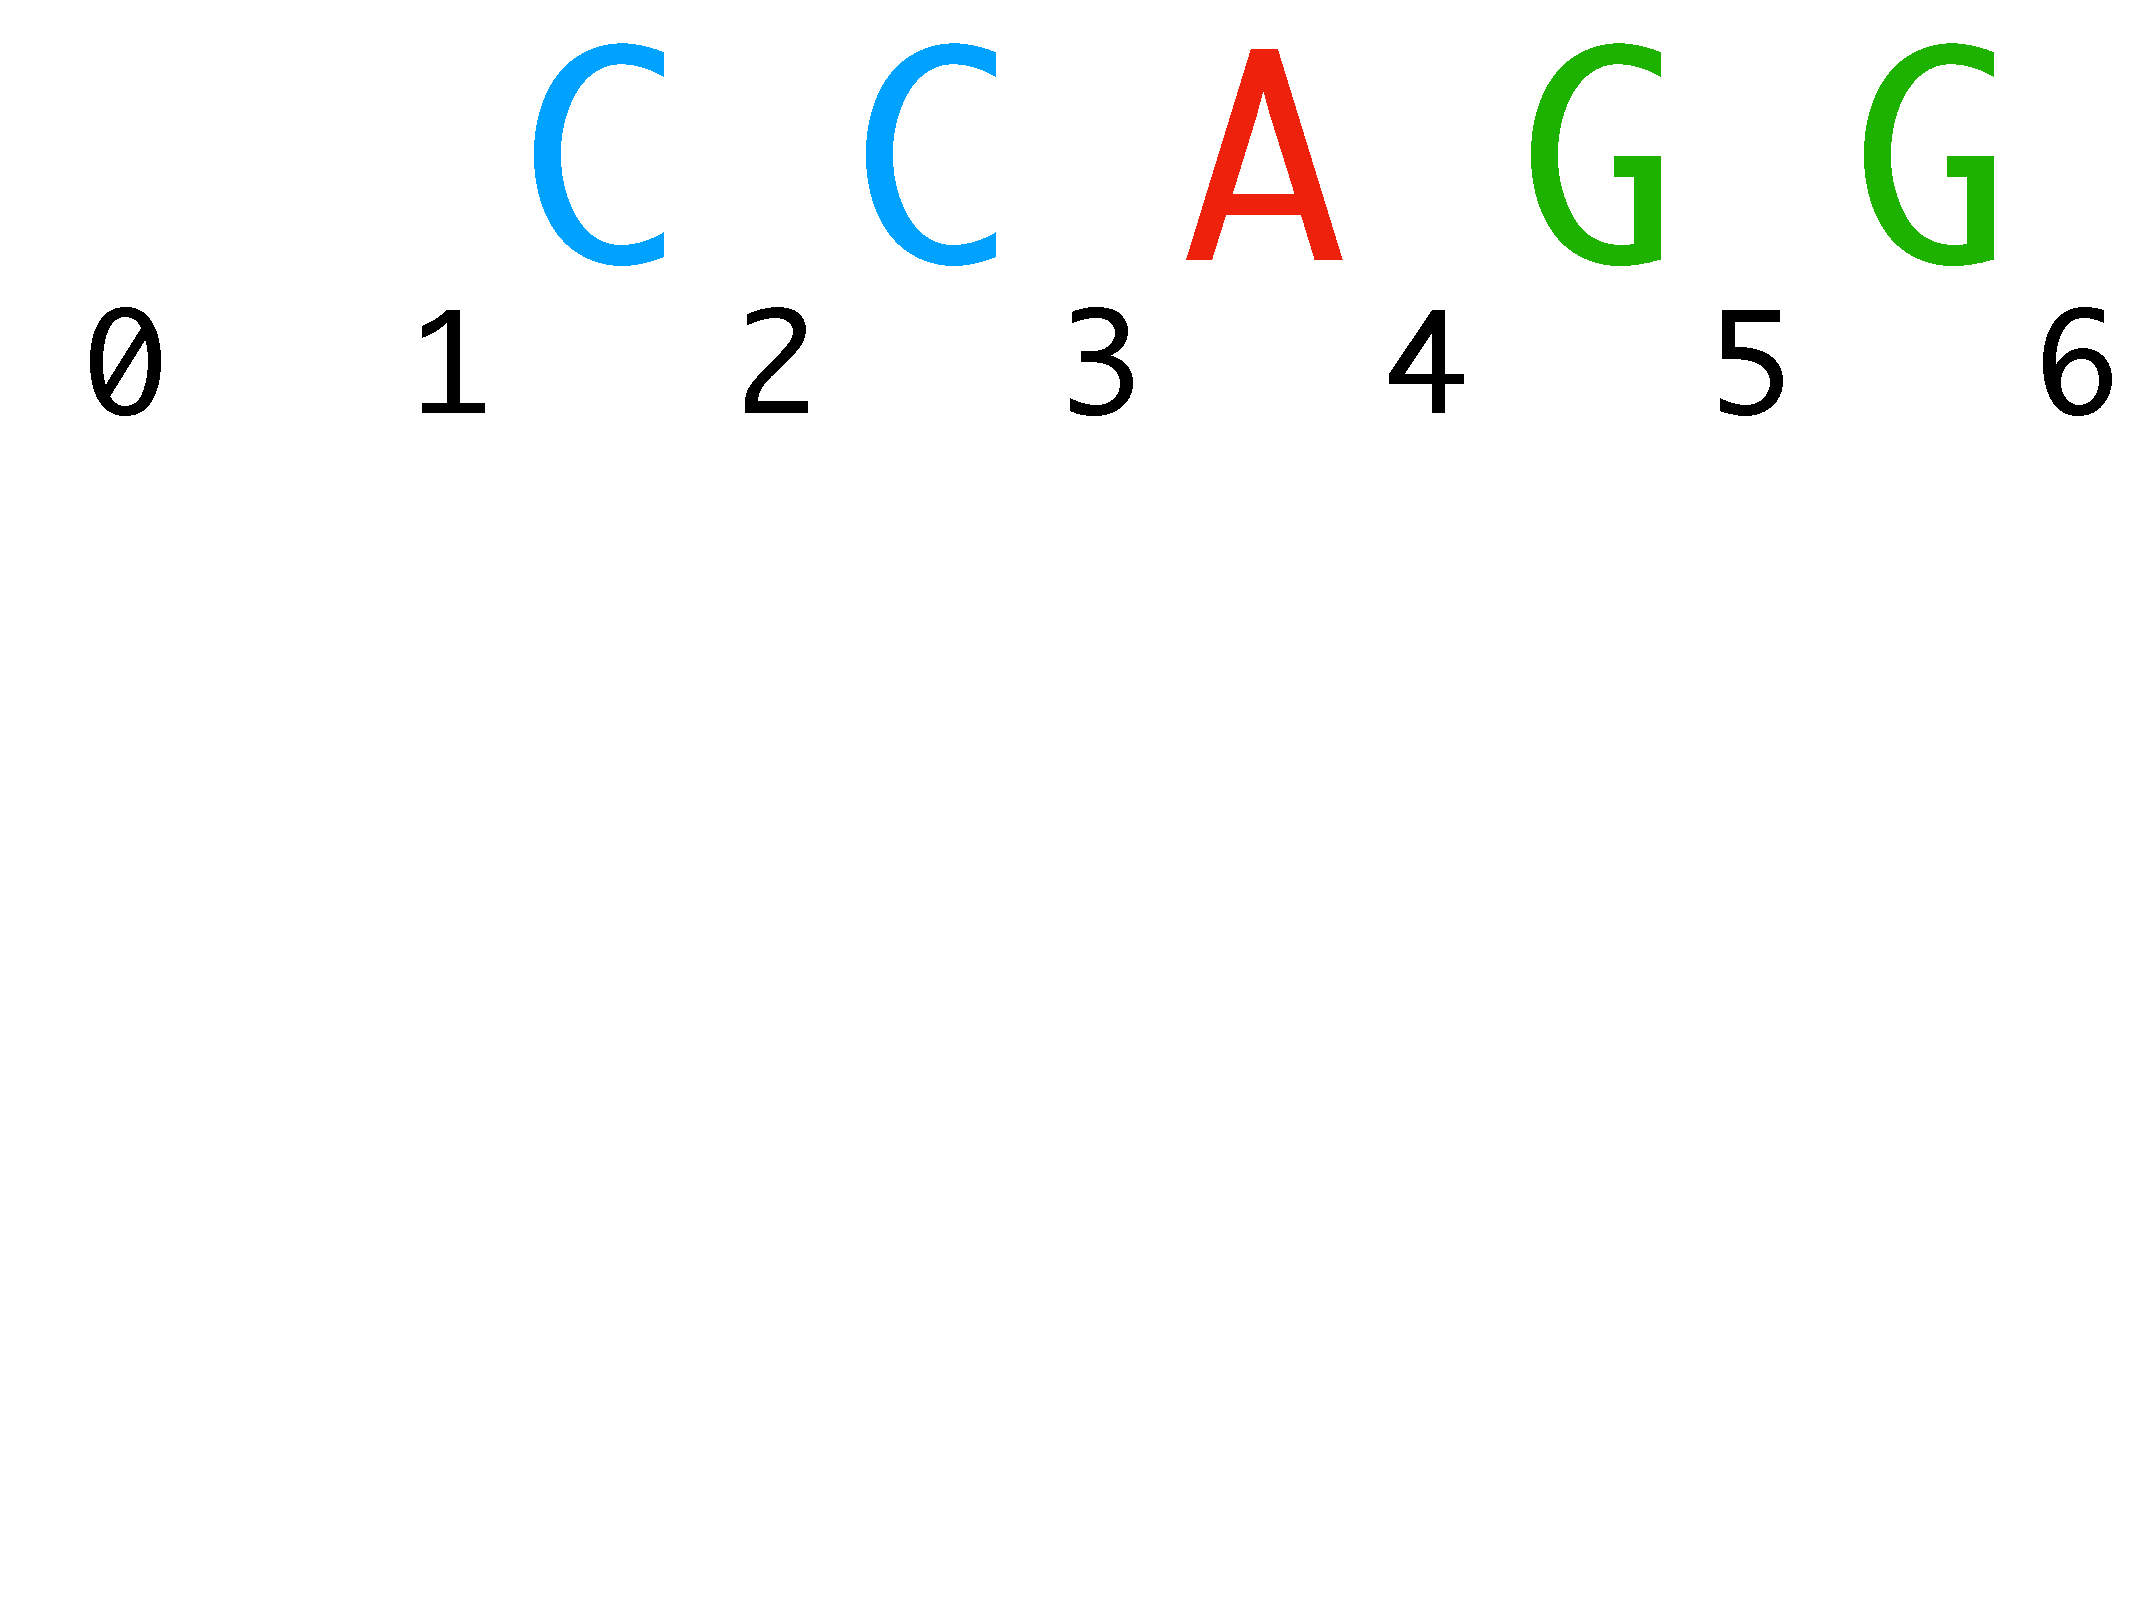
\includegraphics[scale=.16]{figs/index} \\[-3.cm]
%\hspace{-0.23cm}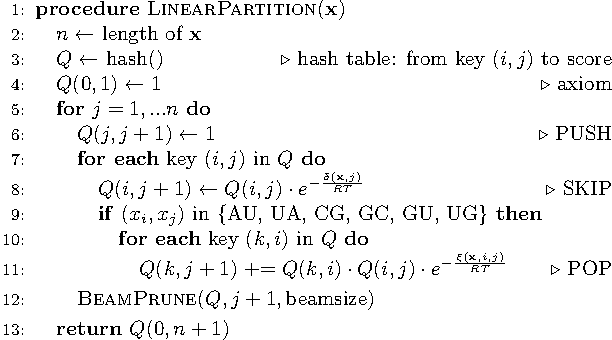
\includegraphics[scale=.83]{figs/algorithm} \\[0.2cm]
\begin{algorithmic}[1]
  \newcommand{\INDSTATE}[1][1]{\State\hspace{#1\algorithmicindent}}
  \setstretch{1.05} % lhuang: usepackage setspace
\Function{LinearPartition}{$\vecx, b$} \Comment{$b$ is the beam size}
% \bindent
    \State $n \gets$ length of $\mathbf x$
    \State $Q \gets$ hash() \Comment{hash table: from span $[i,j]$ to $\Qf{i}{j}$}
    \State $\Qf{j}{j-1} \gets 1$ for all $j$ in $1...n$ \Comment{base cases} \label{line:base}
    \For{$j=1 ... n$}
    \ForEach {$i$ such that $[i,\,j-1]$ in $Q$} \Comment{$O(b)$ iterations}
        \smallskip 
            \State $\Qf{i}{j} \pluseq \Qf{i}{j-1} \cdot e^{-\frac{\delta(\vecx,j)}{RT}} $ \Comment{\nskip} \label{line:skip}
            \If{$x_{i-1}x_j$ in \{AU, UA, CG, GC, GU, UG\}}  \label{line:pair}
                % \State $Q_{i,\,j+1} \gets  C(i,\,j) \cdot e^{-\frac{\xi(\vecx,i,\,j)}{RT}} $
                \ForEach{$k$ such that $[k,\,i-2]$ in $Q$} \Comment{$O(b)$ iters} \smallskip 
                    \State $\Qf{k}{j} \pluseq {\Qf{k}{i-2} \cdot \Qf{i}{j-1} \cdot e^{-\frac{\xi(\vecx,i-1,j)}{RT}}} $ \Comment{\pop} \label{line:pop}
                    % \State $C(0,j+1) \pluseq {C(0,k) \cdot C(k,j+1) \cdot e^{-\frac{\xi(\vecx,i,\,j)}{RT}}} $
                \EndFor
                % \State $C(0,j+1) \pluseq C(0,i) \cdot Q_{i,j+1}$ \Comment{COMBINE}
            \EndIf
        \EndFor
        \State $\textsc {BeamPrune}(Q,j, b)$ \Comment{choose top $b$ out of $Q(\cdot,j)$} \label{line:beamprune}%{see Fig.~\ref{fig:beam_prune_alg}}
        \EndFor
        \vspace{-0.1cm}
    \State \Return $Q$ \Comment{partition function $Q(\vecx)=\Qf{1}{n}$}
% \eindent
\EndFunction
\end{algorithmic}
% \end{algorithm}
\caption{
Partition function calculation pseudocode of a simplified version of the \linearpartition %linear-time partition function calculation
algorithm (the inside phase).
See Fig.~\ref{fig:beam_prune_alg} for the pseudocode of beam pruning (line~\ref{line:beamprune}).
The base-pairing probabilities are computed with the combination of the outside phase
(Fig.~\ref{fig:outside}).
% as well as a beam prune algorithm. 
% Here we model hash tables following Python dictionaries, where $(i, j) \in C$ checks whether the key $(i, j)$ is in the hash $C$; 
% this is needed to ensure linear runtime. 
% Quick select algotithm is used in beam prune, 
% and we skip the details for quick select here since it is well known.
% Real \linearpartition system is much more involved, but the pseudocode illustrates the left-to-right partition function calculation idea using a Nussinov-like fashion.
The actual algorithm using the Turner model is available on \href{https://github.com/LinearFold/LinearPartition}{GitHub}.
%See Fig.~\ref{fig:beam_prune_alg} for {\sc BEAMPRUNE} function.
\label{fig:algorithm}}
\vspace{-.3cm}
% \end{figure*}
\end{figure}


For simplicity of presentation,
in the pseudocode in Fig.~\ref{fig:algorithm}, $Q$ is notated as a hash table,
mapping from  $[i,j]$ to %its partition function
$\Qf{i}{j}$;
see Supplementary Information Section~\ref{sec:si:algdetails} for details
of its efficient implementation. % to make sure the overall runtime is $O(nb^2)$.
As the base case, we set $\Qf{j}{j-1}$ to be 1 for all $j$,
meaning all empty spans have partition function of 1 (line~\ref{line:base}).
%% %to store and look up states.   
%% $\langle 0,1 \rangle:1.0$ represents the dummy head state, 
%% whose partition function $Q(0,1)$ is initialized with value $1$.
%% This represents a structure with no pairs, 
%% i.e., the random coil, 
%% which is the reference state (free energy change of 0) and thus has equilibrium constant of 1.
%% {\color{blue}?????? (added by Mathews, but state <0,1>:1 is a singleton not a coil)}
Our algorithm then scans the sequence from left-to-right (i.e., from 5'-to-3'),
and at each nucleotide $x_j$ ($j=1...n$), % (the length of the sequence), 
% state $\langle 0,j+1 \rangle$ can always be extended with ``\md'' from state $\langle 0,j \rangle$.
% with its 
% Then we define three actions, PUSH, SKIP and POP
% to search states $\langle \cdot,j+1 \rangle$:
we perform two actions: %, \nskip and \pop:
%three actions, PUSH, SKIP and POP, are performed:
% similar as in \linearfold but different 
\begin{itemize}
%% \item PUSH: create a new state $\langle j,j \rangle:1$ representing an open bracket at $j$,
%% whose partition function is 1. 

%% 	% \begin{equation*}
%% 	% 	\frac{\langle i,j \rangle : \Qf{i,j]}{\langle j,j+1 \rangle : 1.0}
%% 	% \end{equation*}

\item \nskip (line~\ref{line:skip}): We extend each %state $[i,\,j-1]: \Qf{i,\,j-1]$ to a new state $[i,j]: \Qf{i,j]$
span $[i,\,j\!-\!1]$ in $Q$ to $[i,j]$ %: \Qf{i,j]$
by adding an unpaired base $y_j\!=$``\md'' (in the dot-bracket notation) to the right of each substructure in $\Qf{i}{j-1}$,
updating $\Qf{i}{j}$: % as follows:
\[
\Qf{i}{j} \pluseq \Qf{i}{j-1} \cdot e^{-\frac{\delta(\vecx, j)}{RT}}
\]
which can be visualized as
%\begin{center}
%  \vspace{-0.7cm}
%  \qquad \qquad
  \begin{tabular}{lr@{\,\quad}} % adjust alignment with j
    \multicolumn{2}{c}{
      $\overbrace{\myboxmath{\ \ \Qf{i}{j-1} \ \ } \ \Huge\md\!\!\!\!}^{\Qf{i}{j}}$
    }
    \\
    $i$ & $j$
  \end{tabular}.
%\end{center}
%% \begin{center}
%%   {

%%     \begin{tabular}{@{}l@{\;}c@{}}
%%       %      \hline
%%       \multicolumn{2}{c}{$\Qf{i,j]$}\\[0.1cm]
%%       \hline
%%   \myboxmath{\quad \Qf{i,j-1]\quad} & {\large\md} \\
%% %  \hline
%%    \multicolumn{1}{l}{$i$} & $j$
%%     \end{tabular}
%% }
%% \end{center}



	% \begin{equation*}
	% 	\frac{\langle i,j \rangle : \Qf{i,j]}{\langle i,j+1 \rangle : \Qf{i,j] \cdot e^{-\frac{\delta(\vecx, j)}{RT}}}
	% \end{equation*}
\vspace{-0.2cm}
\item \pop (lines~\ref{line:pair}--\ref{line:pop}): If $x_{i-1}$ and $x_j$ are pairable,
we combine span $[i,j-1]$ in $Q$ %[i,j]$ 
with each combinable ``left'' span $[k,i-2]$ in $Q$ %: \Qf{k,i-1]$,
% and create a new state $\langle k,j \rangle:Q(k,j)$,
% where $Q(k,j+1)=Q(k,i) \cdot \Qf{i,j] \cdot e^{-\frac{\xi(\vecx, i, j)}{RT}}$.
and update the resulting span $[k,j]$'s partition function % $[k,j+1]: Q(k,j+1)$
%as follows: 
\[
\Qf{k}{j} \pluseq \Qf{k}{i-2} \cdot \Qf{i}{j-1} \cdot e^{-\frac{\xi(\vecx, i-1, j)}{RT}}.
\]
This means that every substructure in $\Qf{i}{j-1}$ can be combined
with every substructure in $\Qf{k}{i-2}$ and a base pair $(i-1, j)$
to form one possible substructure in $\Qf{k}{j}$:
\begin{center}
  \vspace{-0.4cm}
  \begin{tabular}{l@{}r@{}l@{}r@{\,\quad}} %adjust alignment with j
    \multicolumn{4}{c}      
                {$\overbrace{\myboxmath{\; \Qf{k}{i-2}\; } {\Large\ml} \;\; \myboxmath{\; \Qf{i}{j-1}\; } \; {\Large\mr}}^{\Qf{k}{j}}$} \\
  $k$ \hspace{1.15cm} & $i\!-\!1$ & \hspace{0.02cm} {$i$} &  $j$
\end{tabular}
\end{center}
%% \begin{center}
%% \begin{tabular}{l@{}c@{\;}l@{\;}c}
%%   {\myboxmath{\; \Qf{k,i-1]\; }} & \ml & \myboxmath{\quad \Qf{i,j]\quad} & \mr \\
%%   {$x_k$} & $x_{i-1}$ & {$x_i$} & $x_j$
%% \end{tabular}
%% \end{center}

	% \begin{equation*}
	% 	\frac{\langle k,i \rangle : Q(k,i) \ \ \ \ \ \langle i,j \rangle : \Qf{i,j]}{\langle k,j+1 \rangle : Q(k,i) \cdot \Qf{i,j] \cdot e^{-\frac{\xi(\vecx, i, j)}{RT}}}
	% \end{equation*}

% Note that the operator of updating $Q(k,j+1)$ is "+=" (see Figure~\ref{algorithm} line 11).

% \item COMBINE: for each close state $\langle i,j \rangle$, it can be combined with its prefix state $\langle 0,i \rangle$ and form state $\langle 0,j+1 \rangle$:
% 	\begin{equation*}
% 		\frac{\langle 0,i \rangle : Q_{0,i} \ \ \langle i,j \rangle : Q_{i,j}}{\langle 0,j+1 \rangle : Q_{0,i} \cdot Q_{i,j} \cdot e^{-\frac{\xi(\vecx, i, j)}{RT}}}
% 	\end{equation*}
\end{itemize}

Above we presented a simplified version of our left-to-right \linearpartition algorithm. % that resembles \linearfold\/ {\em without} beam pruning.
%Like \linearfold,
We have 
three nested loops, one for $j$, one for $i$, and one for $k$,
and each loop takes at most $n$ iterations; % (i.e., $k,i$ and $j$ are all bounded by $n$).
therefore, the time complexity {\em without} beam pruning is $O(n^3)$,
which is identical to the classical McCaskill Algorithm (see Fig.~\ref{fig:overview}D).
In fact, there is an alternative, bottom-up, interpretation of our left-to-right algorithm
that resembles the Nussinov-style recursion of the classical McCaskill Algorithm:
\vspace{-0.1cm}
\[
\Qf{k}{j} \!=\! \Qf{k}{j-1} \cdot e^{-\frac{\delta(\vecx, j)}{RT}} + \!\! \sum_{k<i\leq j} \!\! {\Qf{k}{i-2} \cdot \Qf{i}{j-1}   \cdot e^{-\frac{\xi(\vecx, i-1, j)}{RT}}}
\]
%% \begin{equation*}
%% 	\begin{split}
%% 		\Qf{k}{j} &= \Qf{k}{j-1} \cdot e^{-\frac{\delta(\vecx, j)}{RT}} \\
%% 		       &+ \sum_{k<i\leq j} {\Qf{k}{i-2} \cdot \Qf{i}{j-1}   \cdot e^{-\frac{\xi(\vecx, i-1, j)}{RT}}}
%% 	\end{split}
%% \end{equation*}



%% % beam prune
%% The pseudocode in Figure~\ref{fig:algorithm} shows that our \linearpartition algorithm has three nested loops, 
%% one for $j$, one for $i$, and one for $k$,
%% and each loop has at most $n$ iterations. % (i.e., $k,i$ and $j$ are all bounded by $n$).
%% Therefore, the  time complexity without beam pruning is $O(n^3)$, which is identical to the classical McCaskill Algorithm,
However, unlike the classical bottom-up McCaskill algorithm,
our left-to-right dynamic programming, inspired by \linearfold, % instead of bottom-up fashion;
%% this is similar to the $O(n^3)$ left-to-right dynamic programming algorithm in \linearfold.
%% This left-to-right dynamic programming
makes it possible to further apply the beam pruning heuristic
%a heuristic method,
to achieve linear runtime in practice.
% and achive linear runtime.
The main idea is, at each step $j$, among all possible spans $[i, j]$ that ends at $j$  (with $i=1...j$), 
we only keep the top $b$ most promising candidates (ranked by their partition functions \Qf{i}{j}).
%i.e., the top $b$ among all \Qf{i}{j}'s,
%those %$(i,j)$
%with higher partition functions, %value $Q_{i,j}$, 
%and remove the other ones
where $b$ is the beam size.
% We adopt quick select algorithm to ensure the process of selecting top $b$  candidates costs linear runtime.
With such beam pruning, 
we reduce the number of states from $O(n^2)$ to $O(nb)$,
and the runtime from $O(n^3)$ to $O(nb^2)$.
For details of the efficient implementation and runtime analysis, please refer to
Supplementary Information Section~\ref{sec:si:algdetails}.
Note $b$ is a user-adjustable constant ($b=$100 by default).


After the partition-function calculation, also known as the ``inside'' phase of the classical inside-outside algorithm~\cite{baker:1979},
we design a similar linear-time ``outside'' phase (see Supplementary Section~\ref{sec:outside})
to compute the base pairing probabilities:
\vspace{-0.1cm}
\[
p_{i,j} = \sum_{(i,j)\in \pairs(\vecy)} p(\vecy),
\]
where $p_{i,j}$ is the probability of nucleotide $i$ pairing with $j$,
which sums the probabilities of all structures that contain $(i,j)$ pair,
and $p(\vecy)=e^{-\frac{\Delta G^\circ(\vecy)}{RT}} / Q(\vecx)$
is the probability of structure \vecy % of the structure $\vecy$ in the ensemble.
in the ensemble.  %among all possible structures
%(or the probability of $i$ being unpaired when $j=N+1$).





\subsection{Efficiency and Scalability}
% !TEX root = main.tex

\begin{figure}[t]
\center
% \includegraphics[scale=1.]{figs/runtime_desktop_bpp_vienna_b2}
\begin{tabular}{cc}
\hspace{-4.5cm}{\panel{A}} & \hspace{-4.8cm}{\panel{B}} \\[-0.5cm]
\hspace{-.2cm}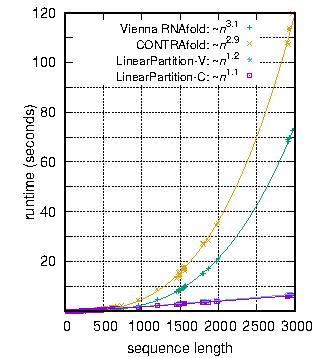
\includegraphics[scale=.9]{figs/runtime_desktop_overall_4sys_log_new}
&
\hspace{-.6cm}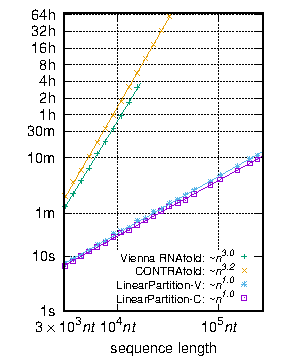
\includegraphics[scale=.9]{figs/rnacentral_desktop_runtime} \\[-1.8cm]
\hspace{-4.5cm}\raisebox{4.cm}{\panel{C}} & \hspace{-5.5cm}{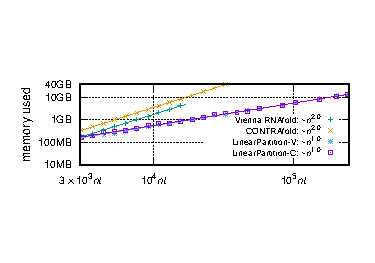
\includegraphics[scale=1.35]{figs/mem}} \\[-2.1cm]
% \multicolumn{2}{c}{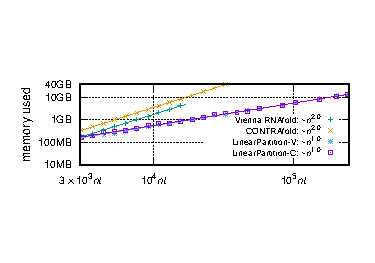
\includegraphics[scale=1.35]{figs/mem}} \\[-1.1cm]
\end{tabular}
\caption{Total runtime and memory usage of computing both the partition function and base pairing probabilities. % running speed and space comparisons.
% Runtime comparisons on ArchiveII and RNAcentral datasets, and memory usage comparison on RNAcentral dataset. 
{\bf A}: Runtime comparisons on the ArchiveII dataset; the curve-fittings were log-log in gnuplot with $n > 10^3$.
{\bf B}: Runtime comparisons on the RNAcentral dataset (log scale). %; the x-axis and y-axis are in log scale. 
%% Note that we show the total runtime of computing both the partition function and base pairing probabilities,
%% where the former takes about half of the time.
The partition function computation takes about half of the total time shown here.
% \viennarnafold overflows on the sequence of 19,071~\nts. 
% time limit is 24 hours.
{\bf C}: Memory usage comparisons on the RNAcentral dataset (log scale).
\label{fig:runtime}}
\vspace{-0.5cm}
\end{figure}



We present two versions of \linearpartition:
{\em \linearpartitionv}
using thermodynamic parameters~\cite{mathews+:1999,Mathews+:2004,xia+:1998}
%as implemented in
following \viennarnafold~\cite{lorenz+:2011},
and
{\em \linearpartitionc} using
the learning-based parameters from \contrafold~\cite{do+:2006}.
%% \linearpartitionv uses the experiment-based thermodynamic parameters~\cite{mathews+:1999,Mathews+:2004,xia+:1998}
%% as implemented in \viennarnafold~\cite{lorenz+:2011}.
%% % (Version 2.4.11) 
%% % (\url{https://www.tbi.univie.ac.at/RNA/download/sourcecode/2_ 4_x/ViennaRNA-2.4.11.tar.gz}).
%% \linearpartitionc uses the machine learning-based parameter values from \contrafold~\cite{do+:2006}.
% (Version 2.0.2; 
% (\url{http://contra.stanford.edu/}).
% \viennarnafold is a widely-used RNA structure prediction package,
% while \contrafold is a successful machine learning-based RNA structure prediction system.
% Both provide partition function and base pairing probabilities calculation based on 
% the classical cubic runtime algorithm.
% Our comparisons mainly focus on the systems with the same model, 
% i.e., \linearpartitionv vs. \viennarnafold and \linearpartitionc vs. \contrafold.
% In this way the differences are based on algorithms themselves rather than models.
% bugs in contrafold
% We found a non-trival bug in \contrafold by comparing our results to CONTRAfold, 
% which leads to overcounting in multiloops in the partition function calculation.
% We corrected the bug, and all experiments are based on this bug-fixed version of \contrafold.
We use %run all evaluations %experiments 
% (compiled by GCC 4.9.0) 
a Linux machine 
with 2.90GHz Intel i9-7920X CPU and 64G memory for benchmarks.
We use sequences from two datasets, ArchiveII~\cite{mathews+:1999, sloma+mathews:2016} and RNAcentral~\cite{rnacentral:2017}. See~\ref{sec:datasets} for details of the datasets.


\begin{figure*}[!htb]
\centering
  \vspace{-1.7cm}
  \begin{tabular}{cccc}
    % \raisebox{4.5cm}
    \raisebox{3.8cm}{\panel{A}} &
    {\hspace{-0.cm}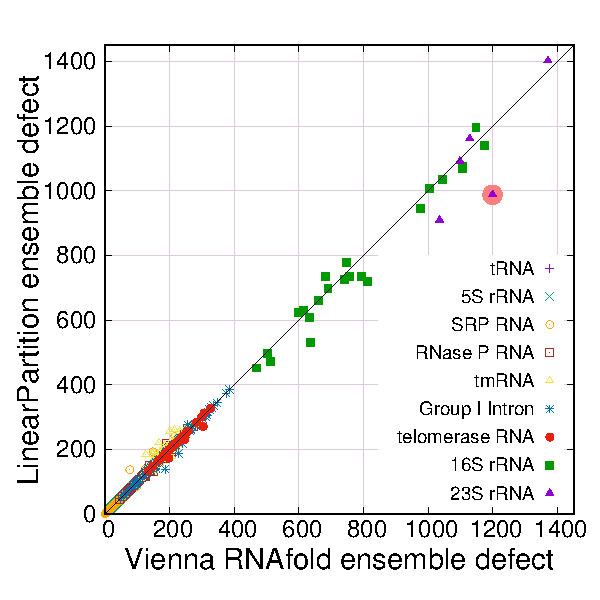
\includegraphics[width=0.24\textwidth]{figs/ensemble_defect}} &
    \raisebox{3.8cm}{\hspace{1.4cm}\panel{B}} &
    \raisebox{-0.3cm}{\hspace{-1.2cm}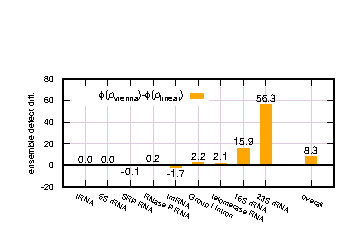
\includegraphics[width=0.5\textwidth]{figs/ensemble_defect_histogram}}
  \end{tabular}
  \\[-0.4cm]
%   \vspace{-.5cm}
  \begin{tabular}{ccccc}
&\hspace{-4.cm} \panel{C} & \hspace{-4.6cm}\panel{D} & \hspace{-4.6cm}\panel{E} & \hspace{-4.6cm}\panel{F}\\[-0.3cm]
\raisebox{.9cm}{\rotatebox{90}{\ecoli 23S rRNA}}&
\hspace{-0.2cm}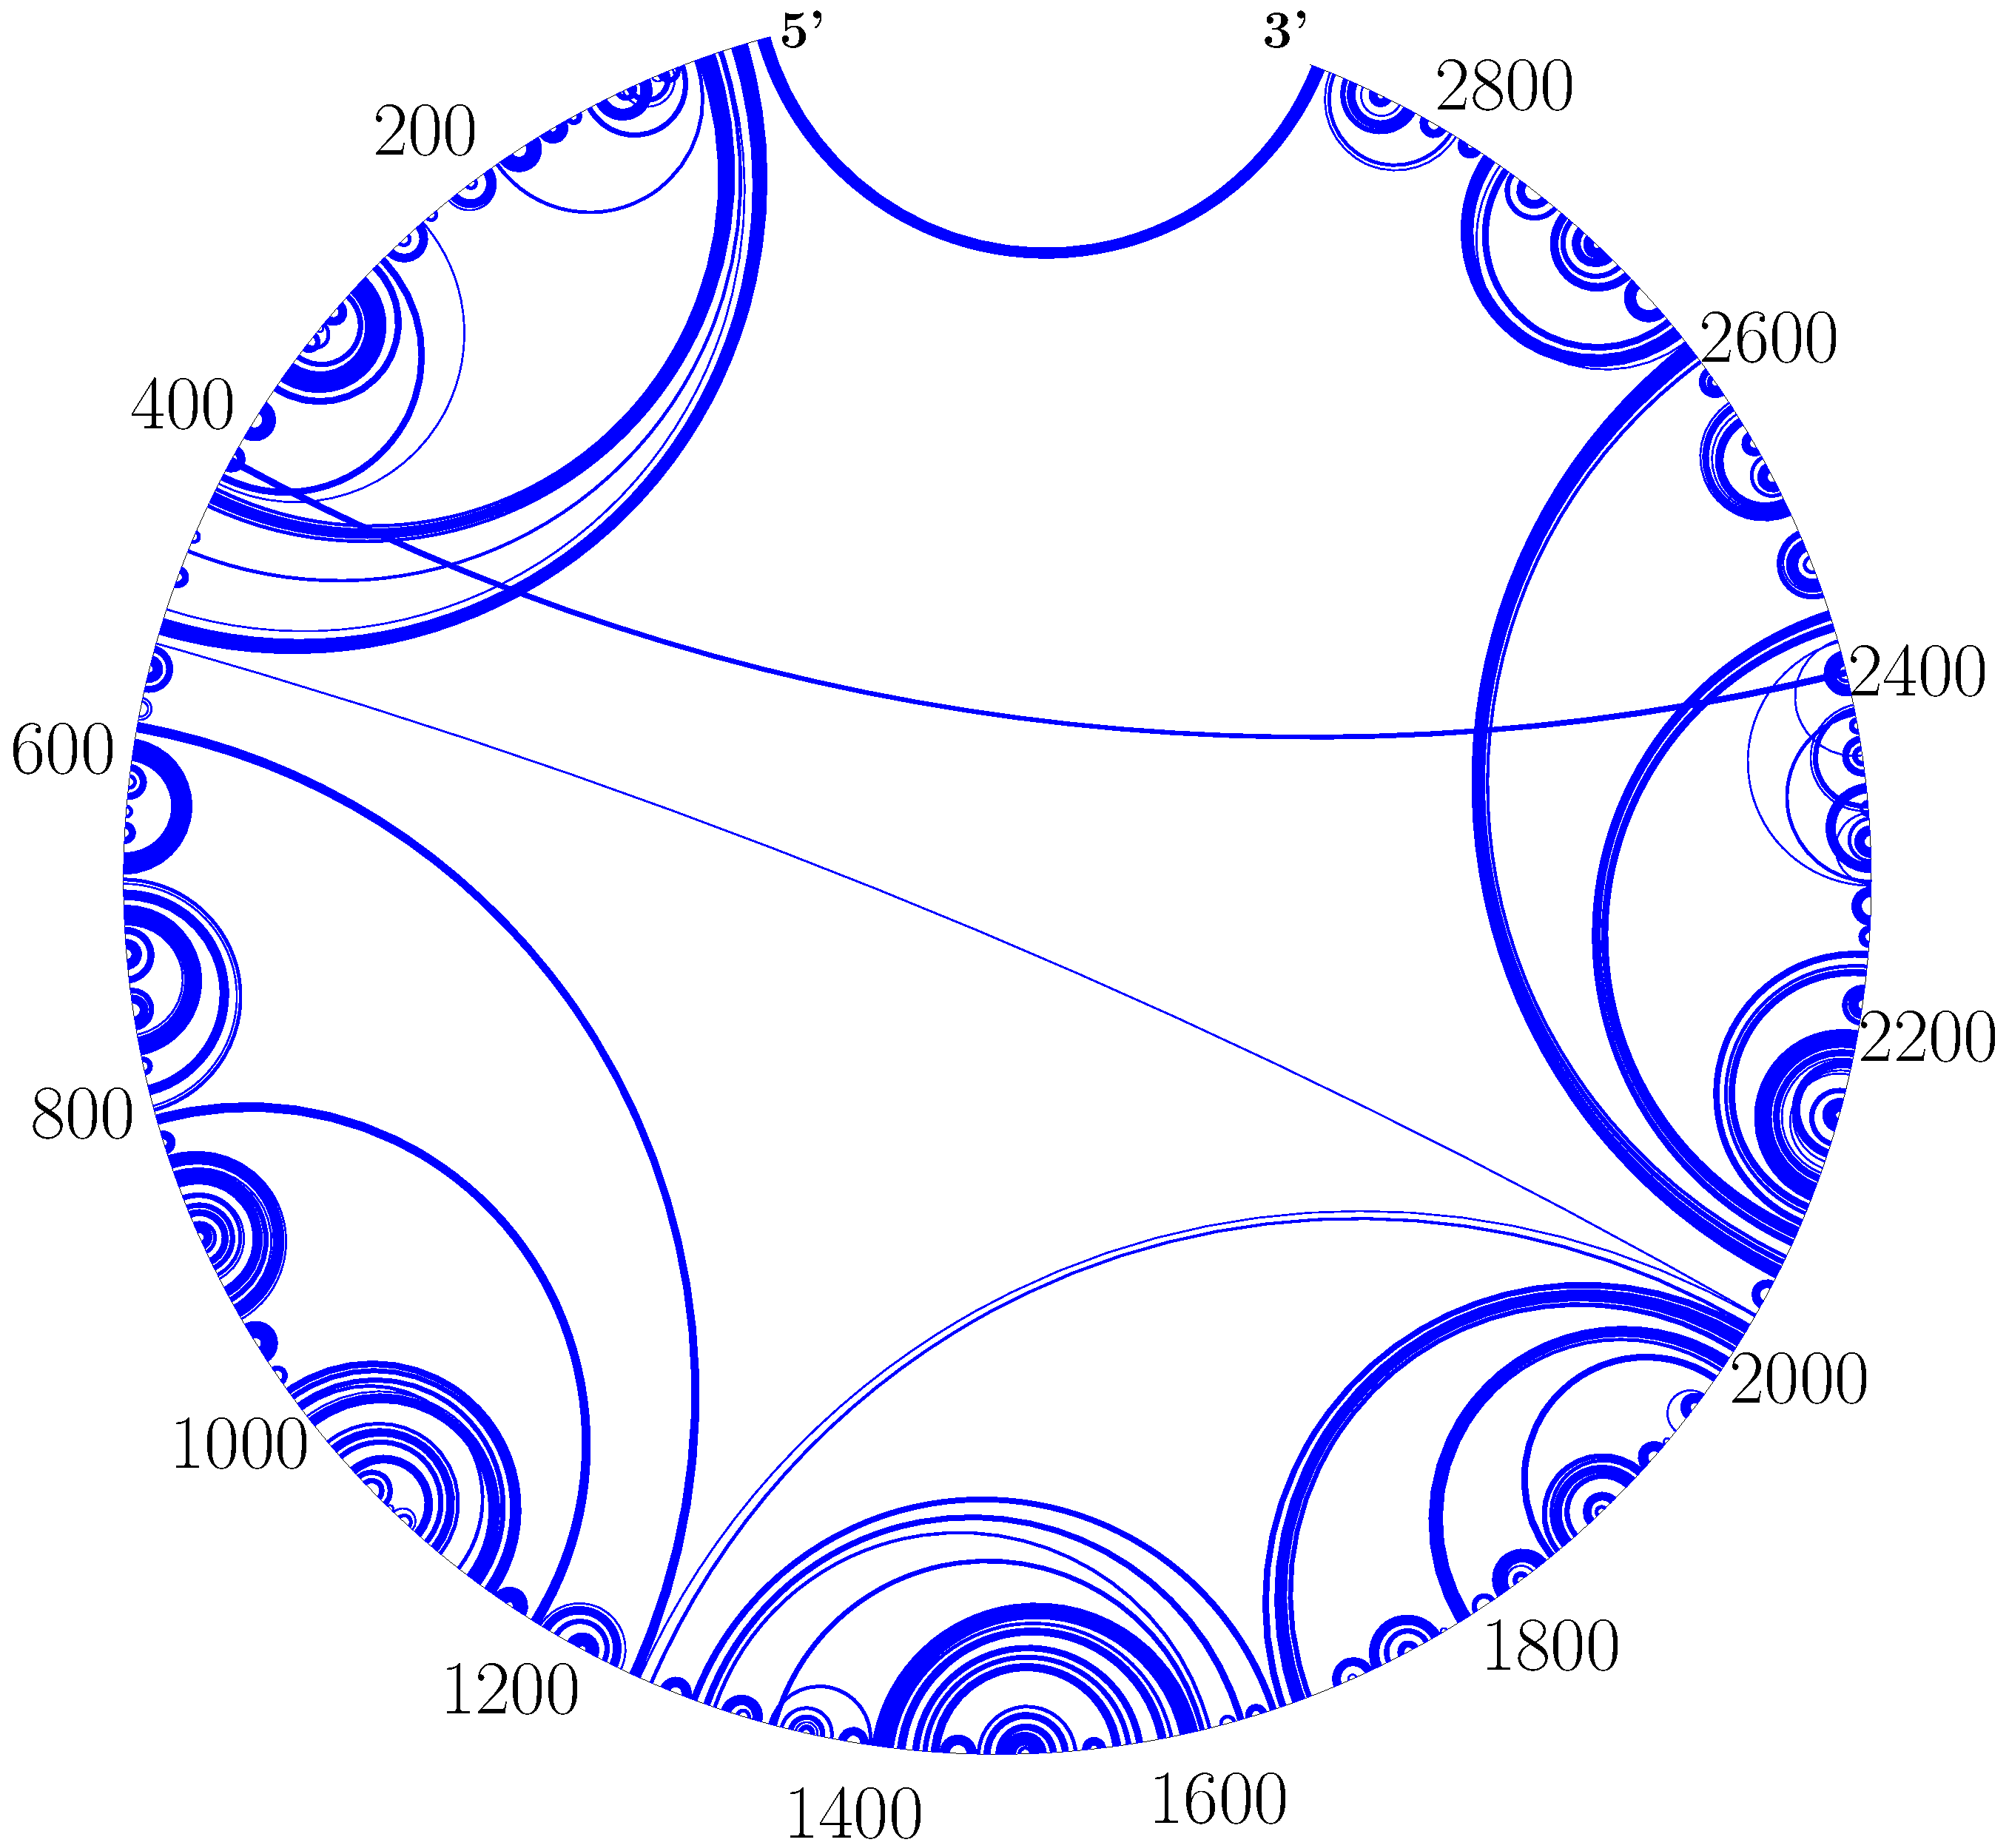
\includegraphics[width=0.22\textwidth]{figs/23s_gold} &
\hspace{-0.35cm}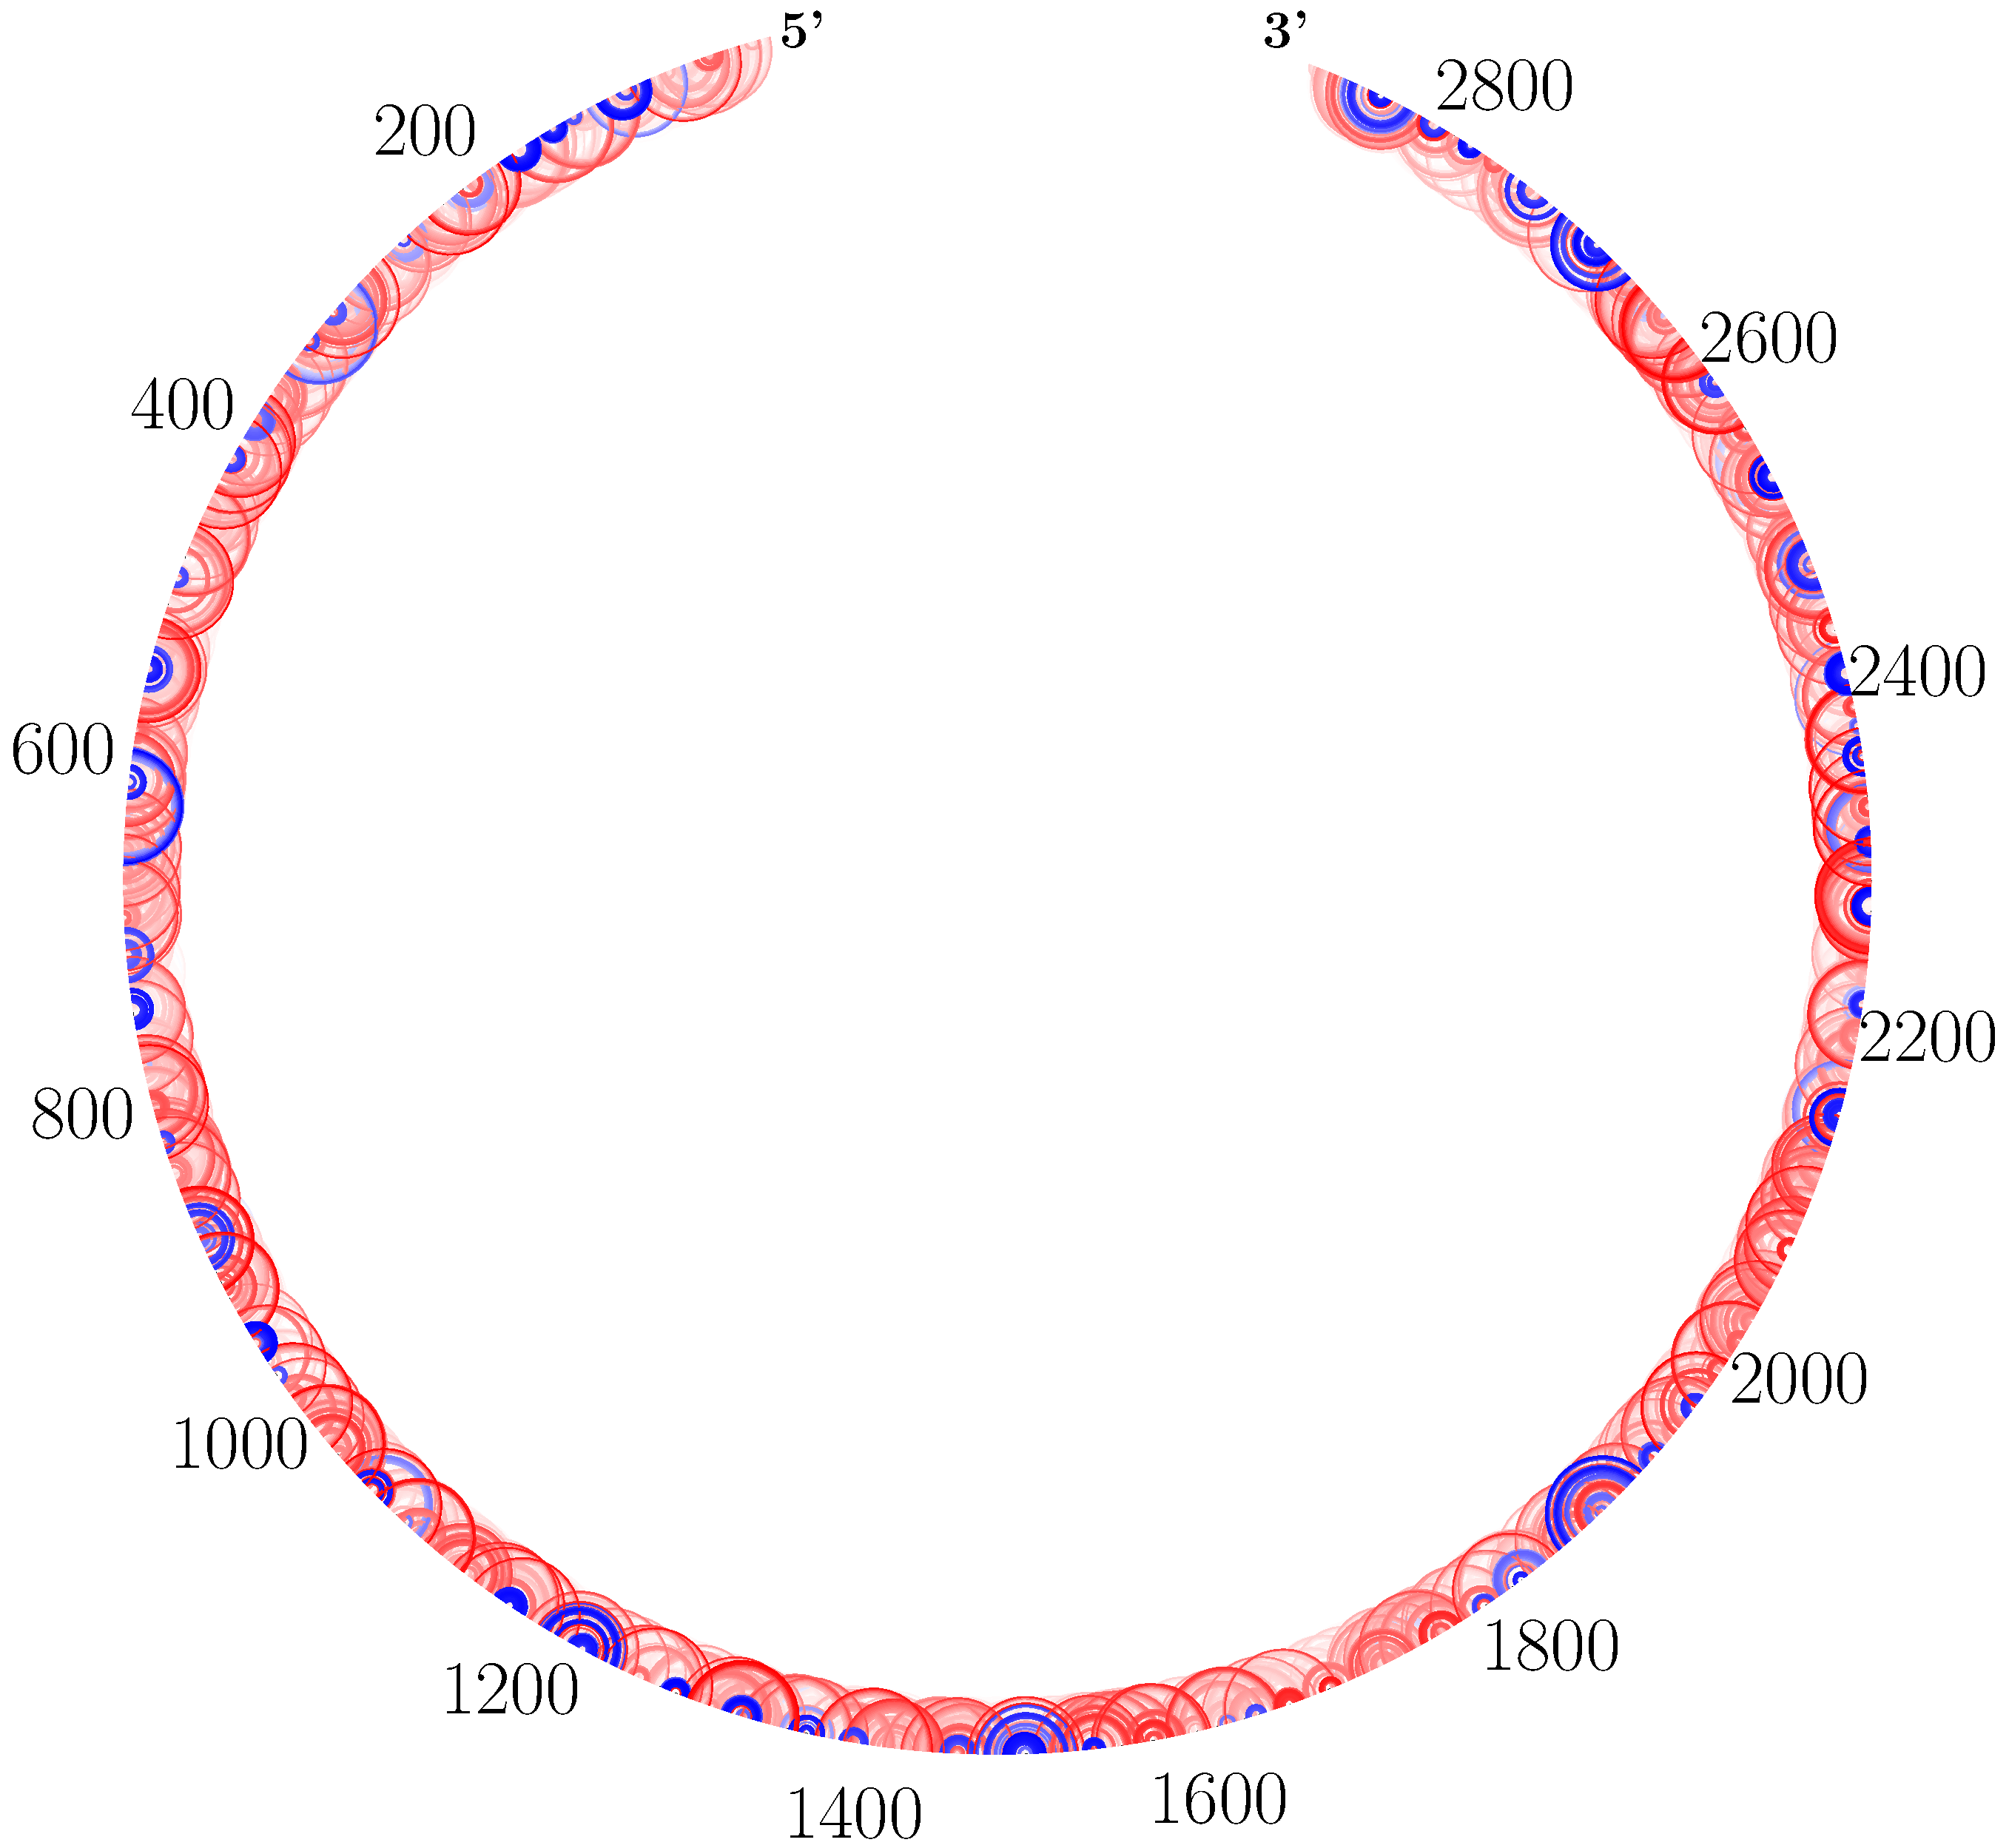
\includegraphics[width=0.22\textwidth]{figs/23s_vienna_plfold_example.pdf} &
\hspace{-0.35cm}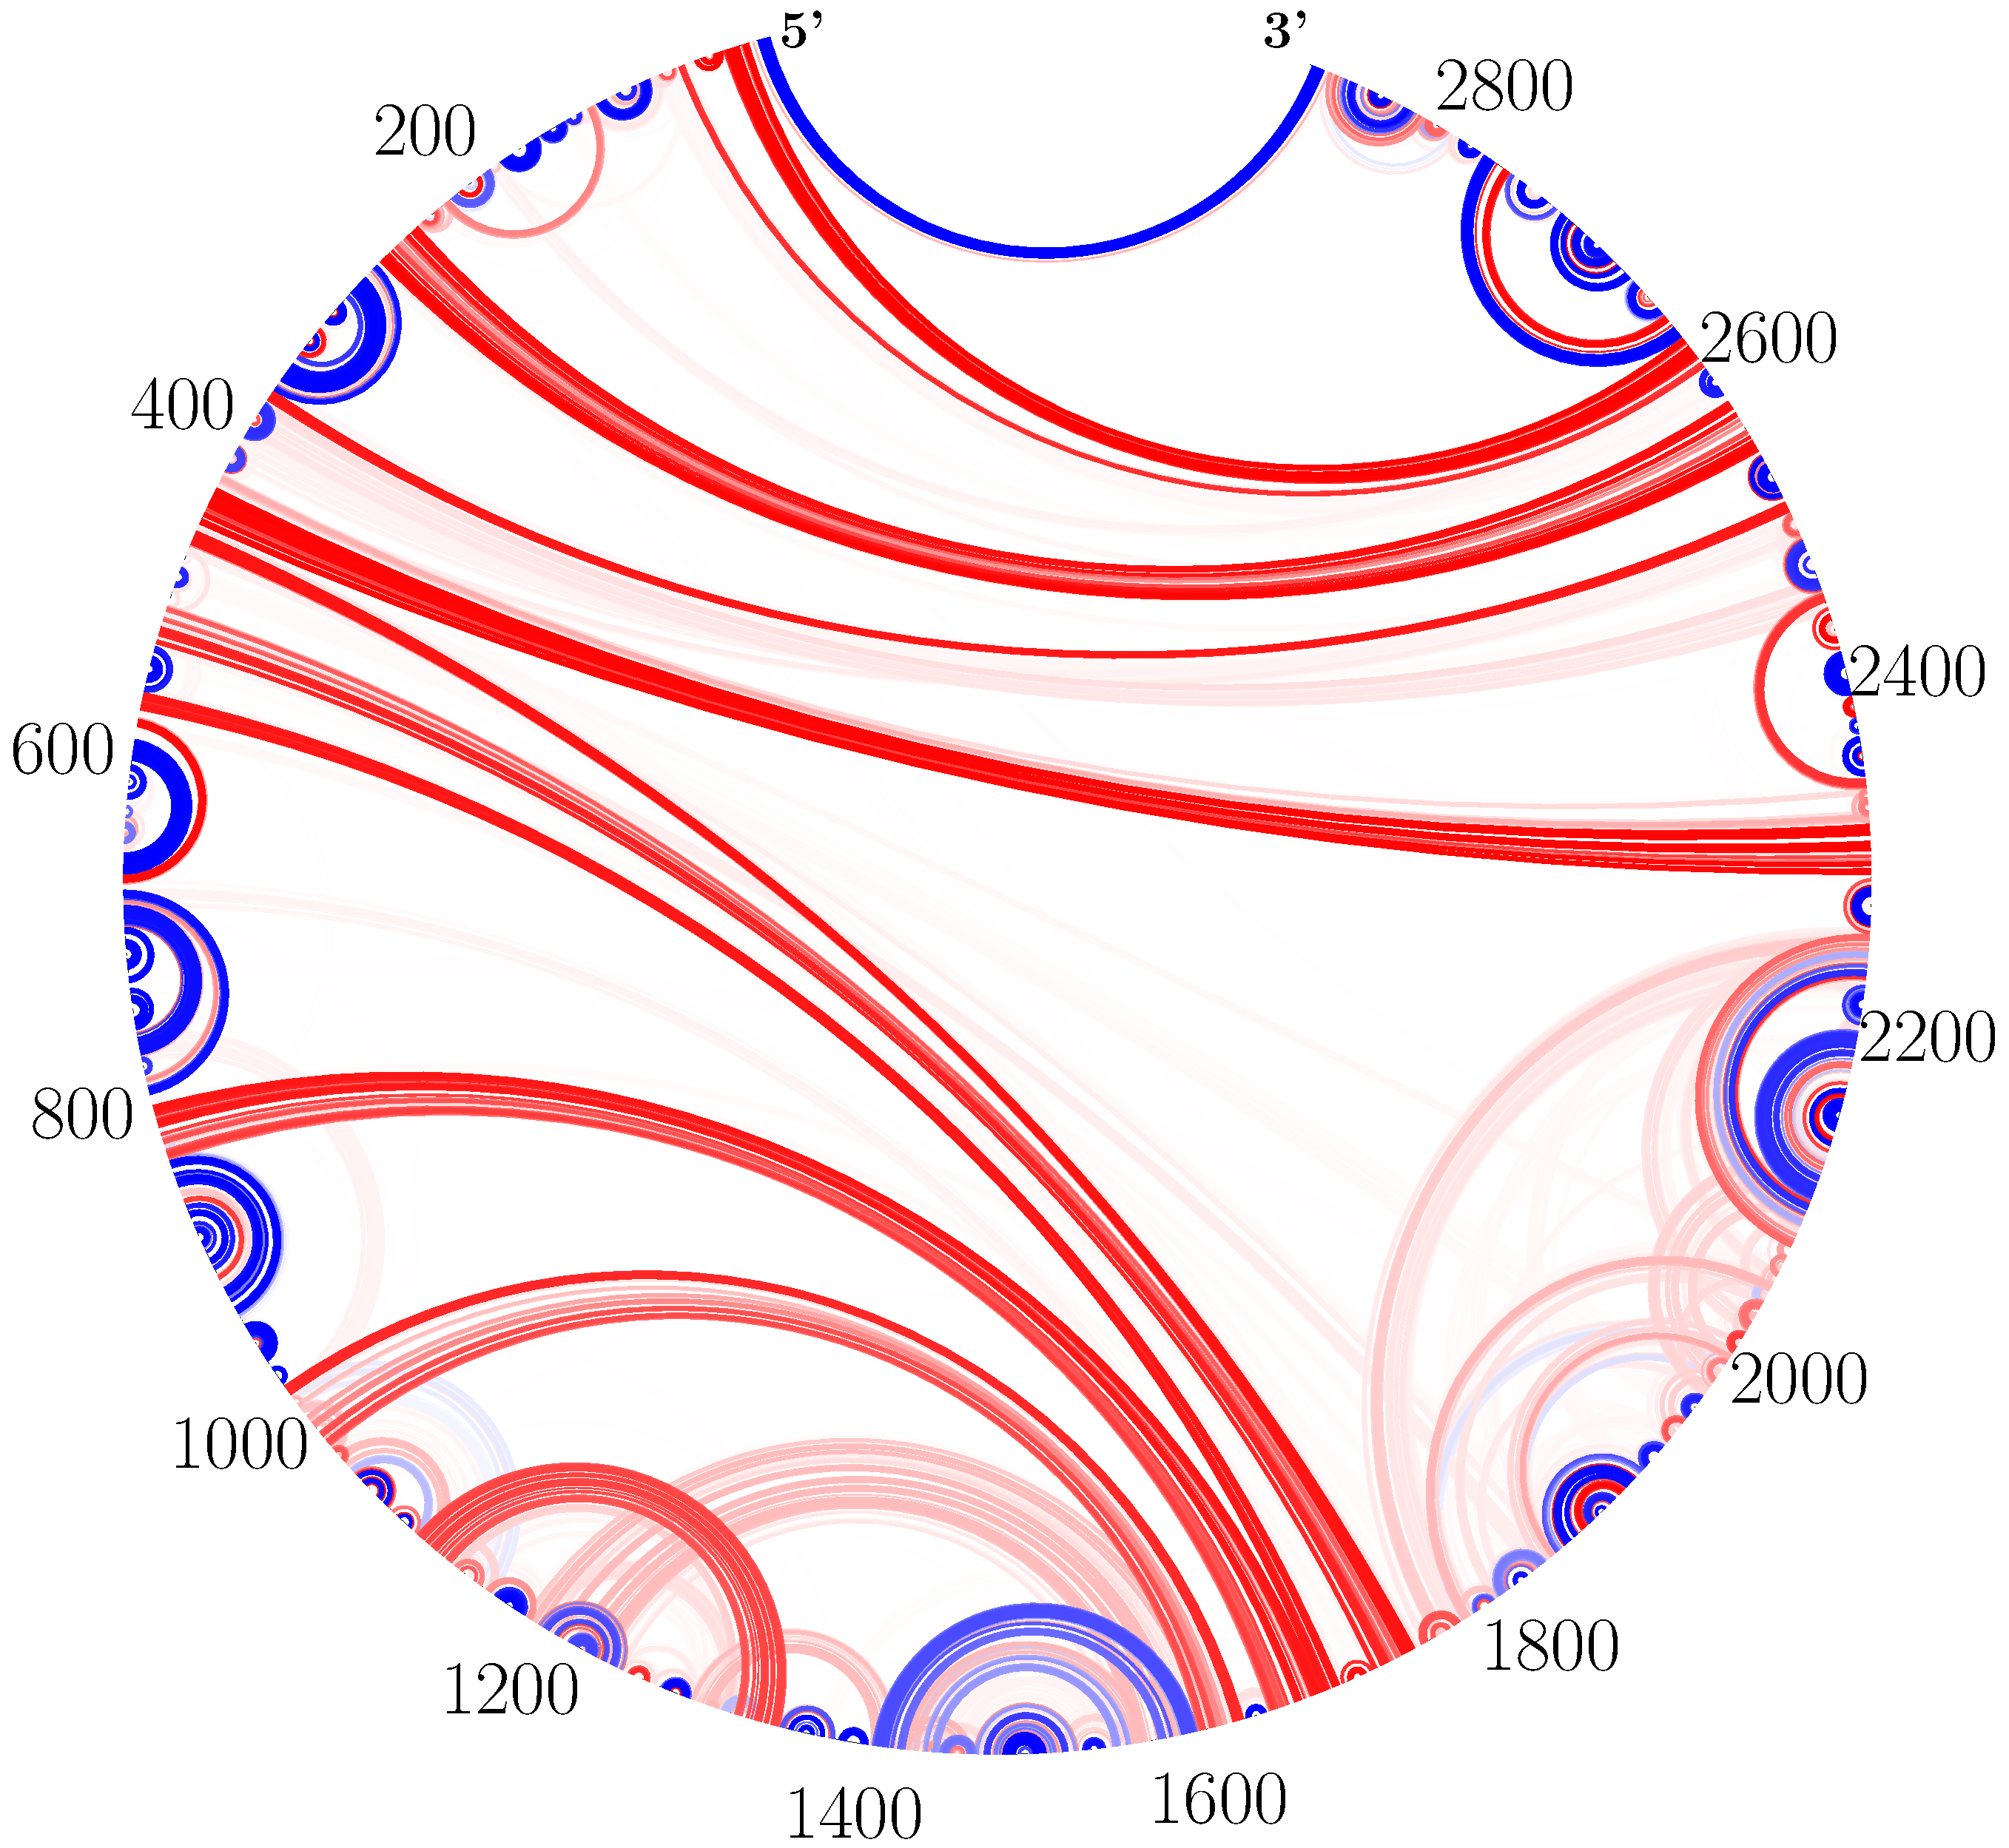
\includegraphics[width=0.22\textwidth]{figs/23s_vienna_example} &
\hspace{-0.35cm}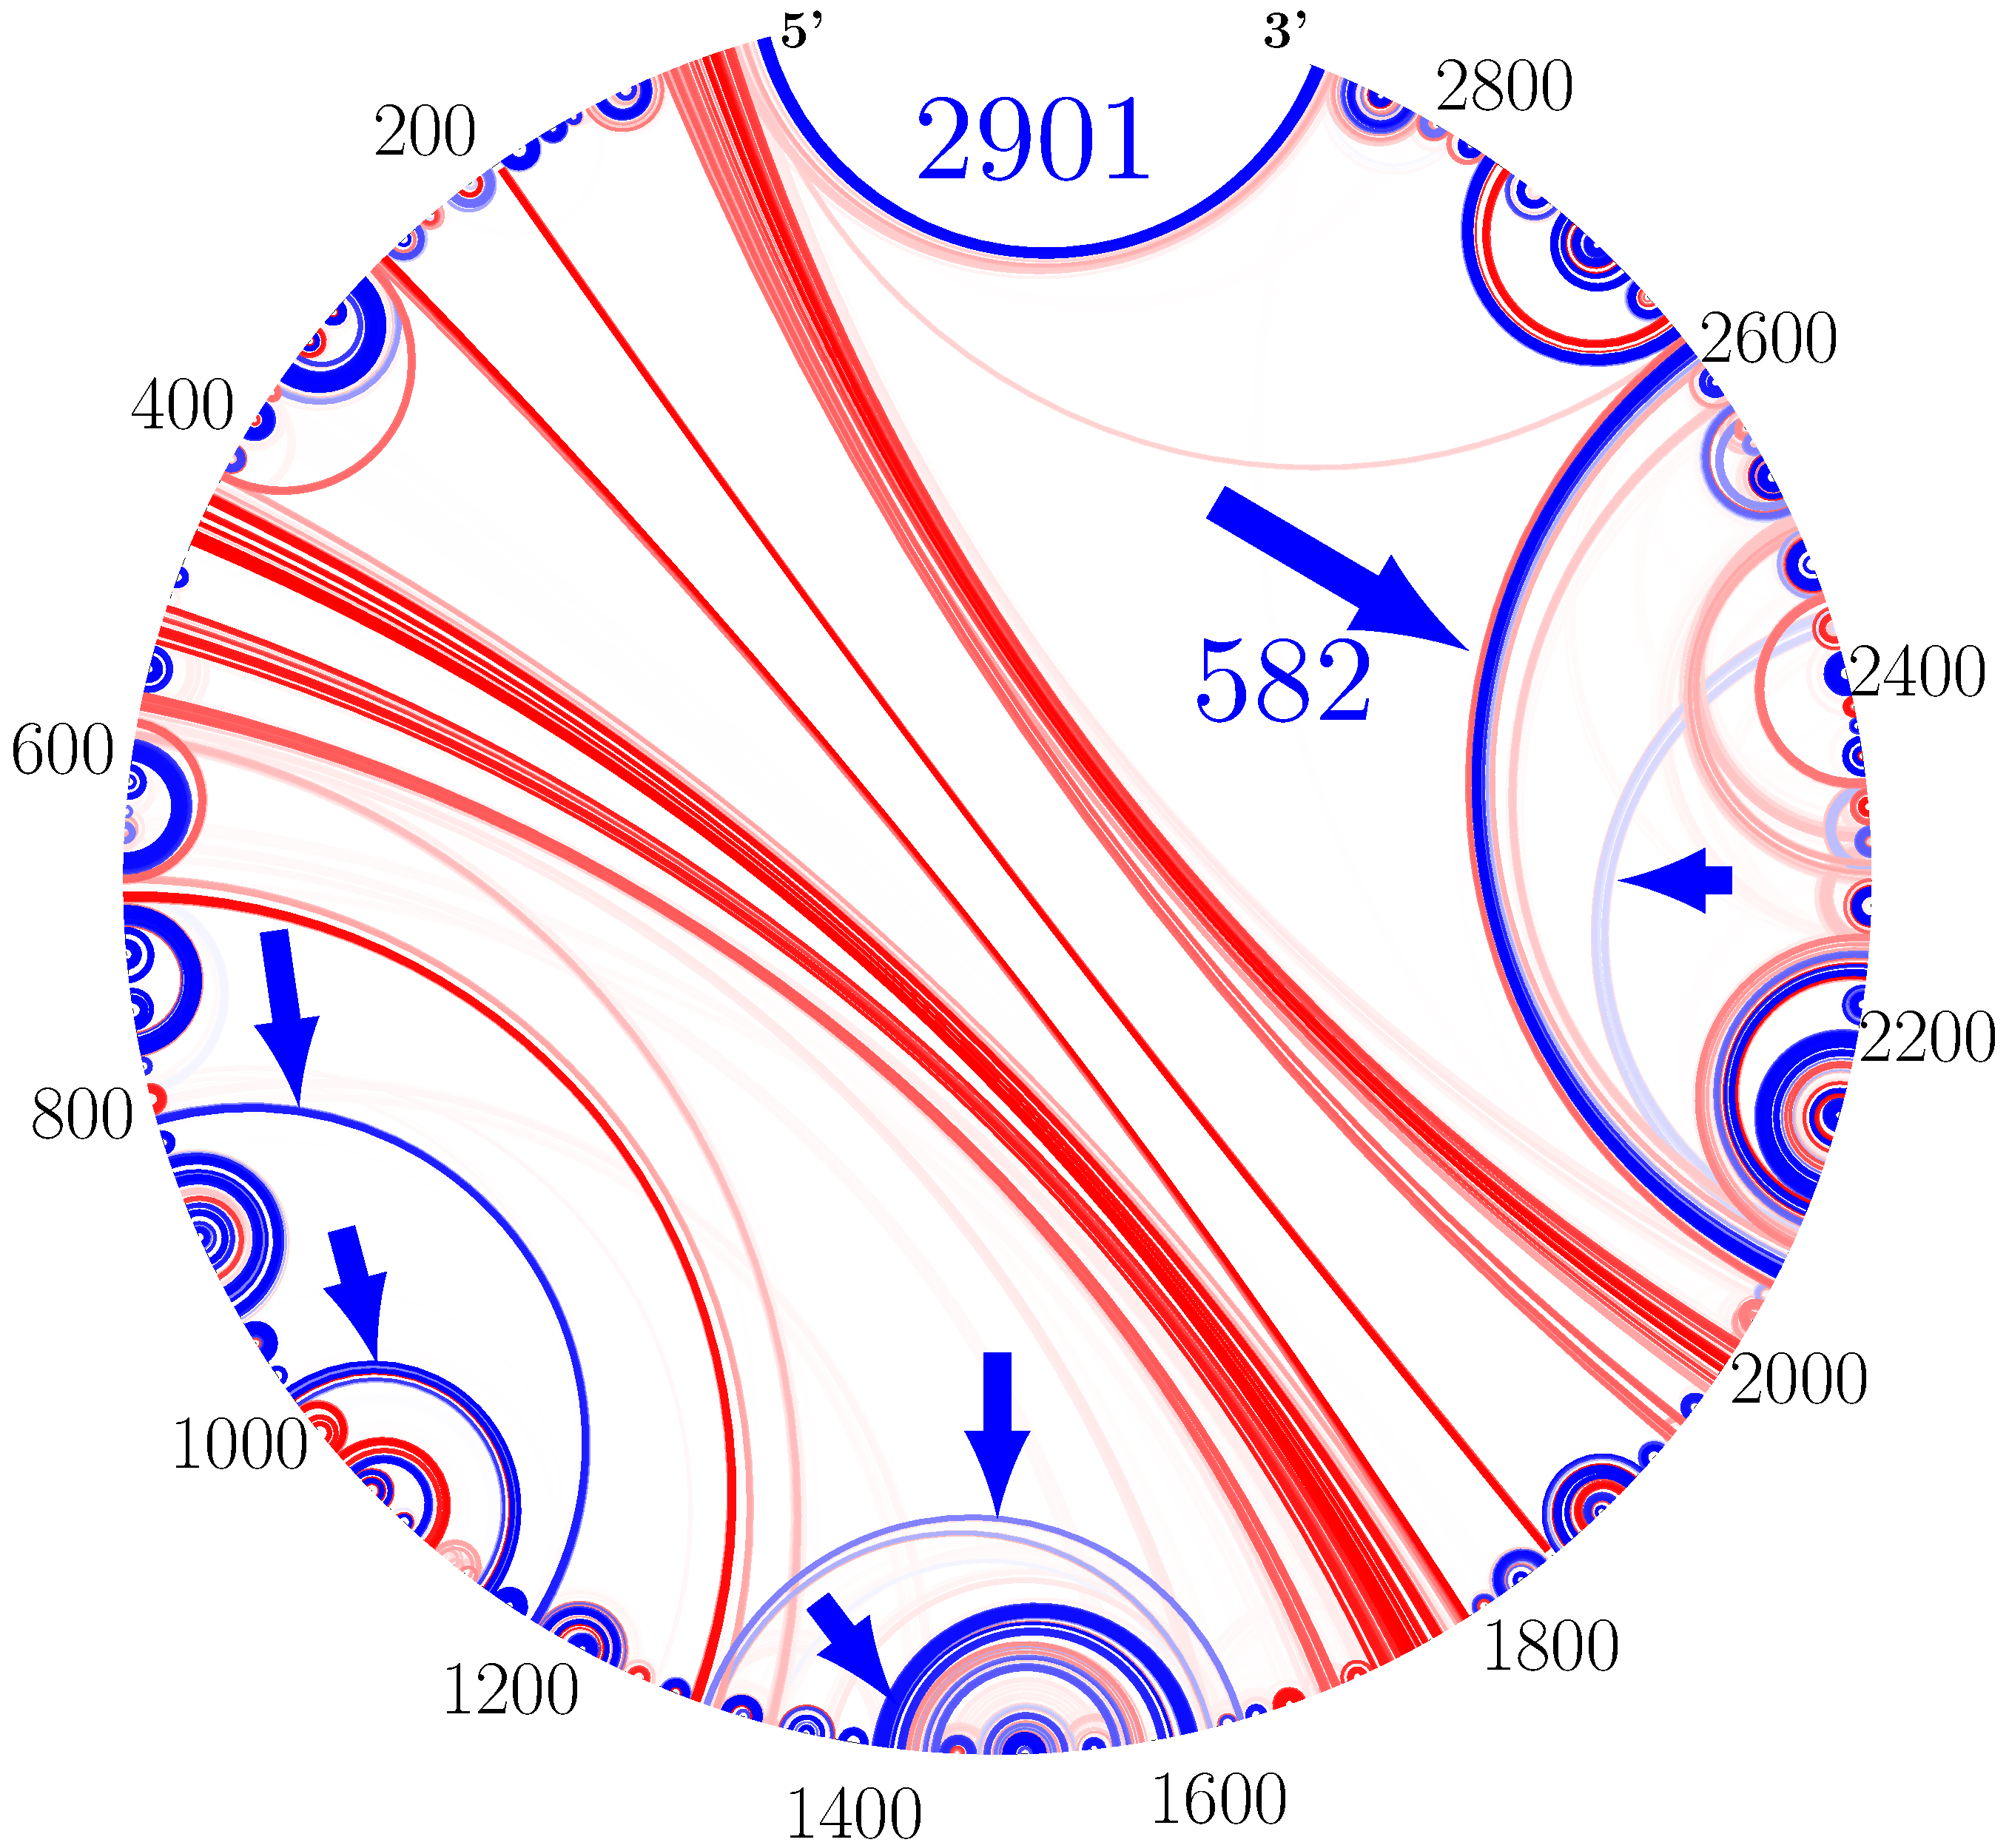
\includegraphics[width=0.22\textwidth]{figs/23s_example.pdf} \\
&\hspace{-4.cm} \panel{G} & \hspace{-4.6cm}\panel{H} & \hspace{-4.6cm}\panel{I} & \hspace{-4.6cm}\panel{J}\\[-0.4cm]
\raisebox{.4cm}{\rotatebox{90}{{\it C.~ellipsoidea} Group I Intron}}&
\hspace{-0.2cm}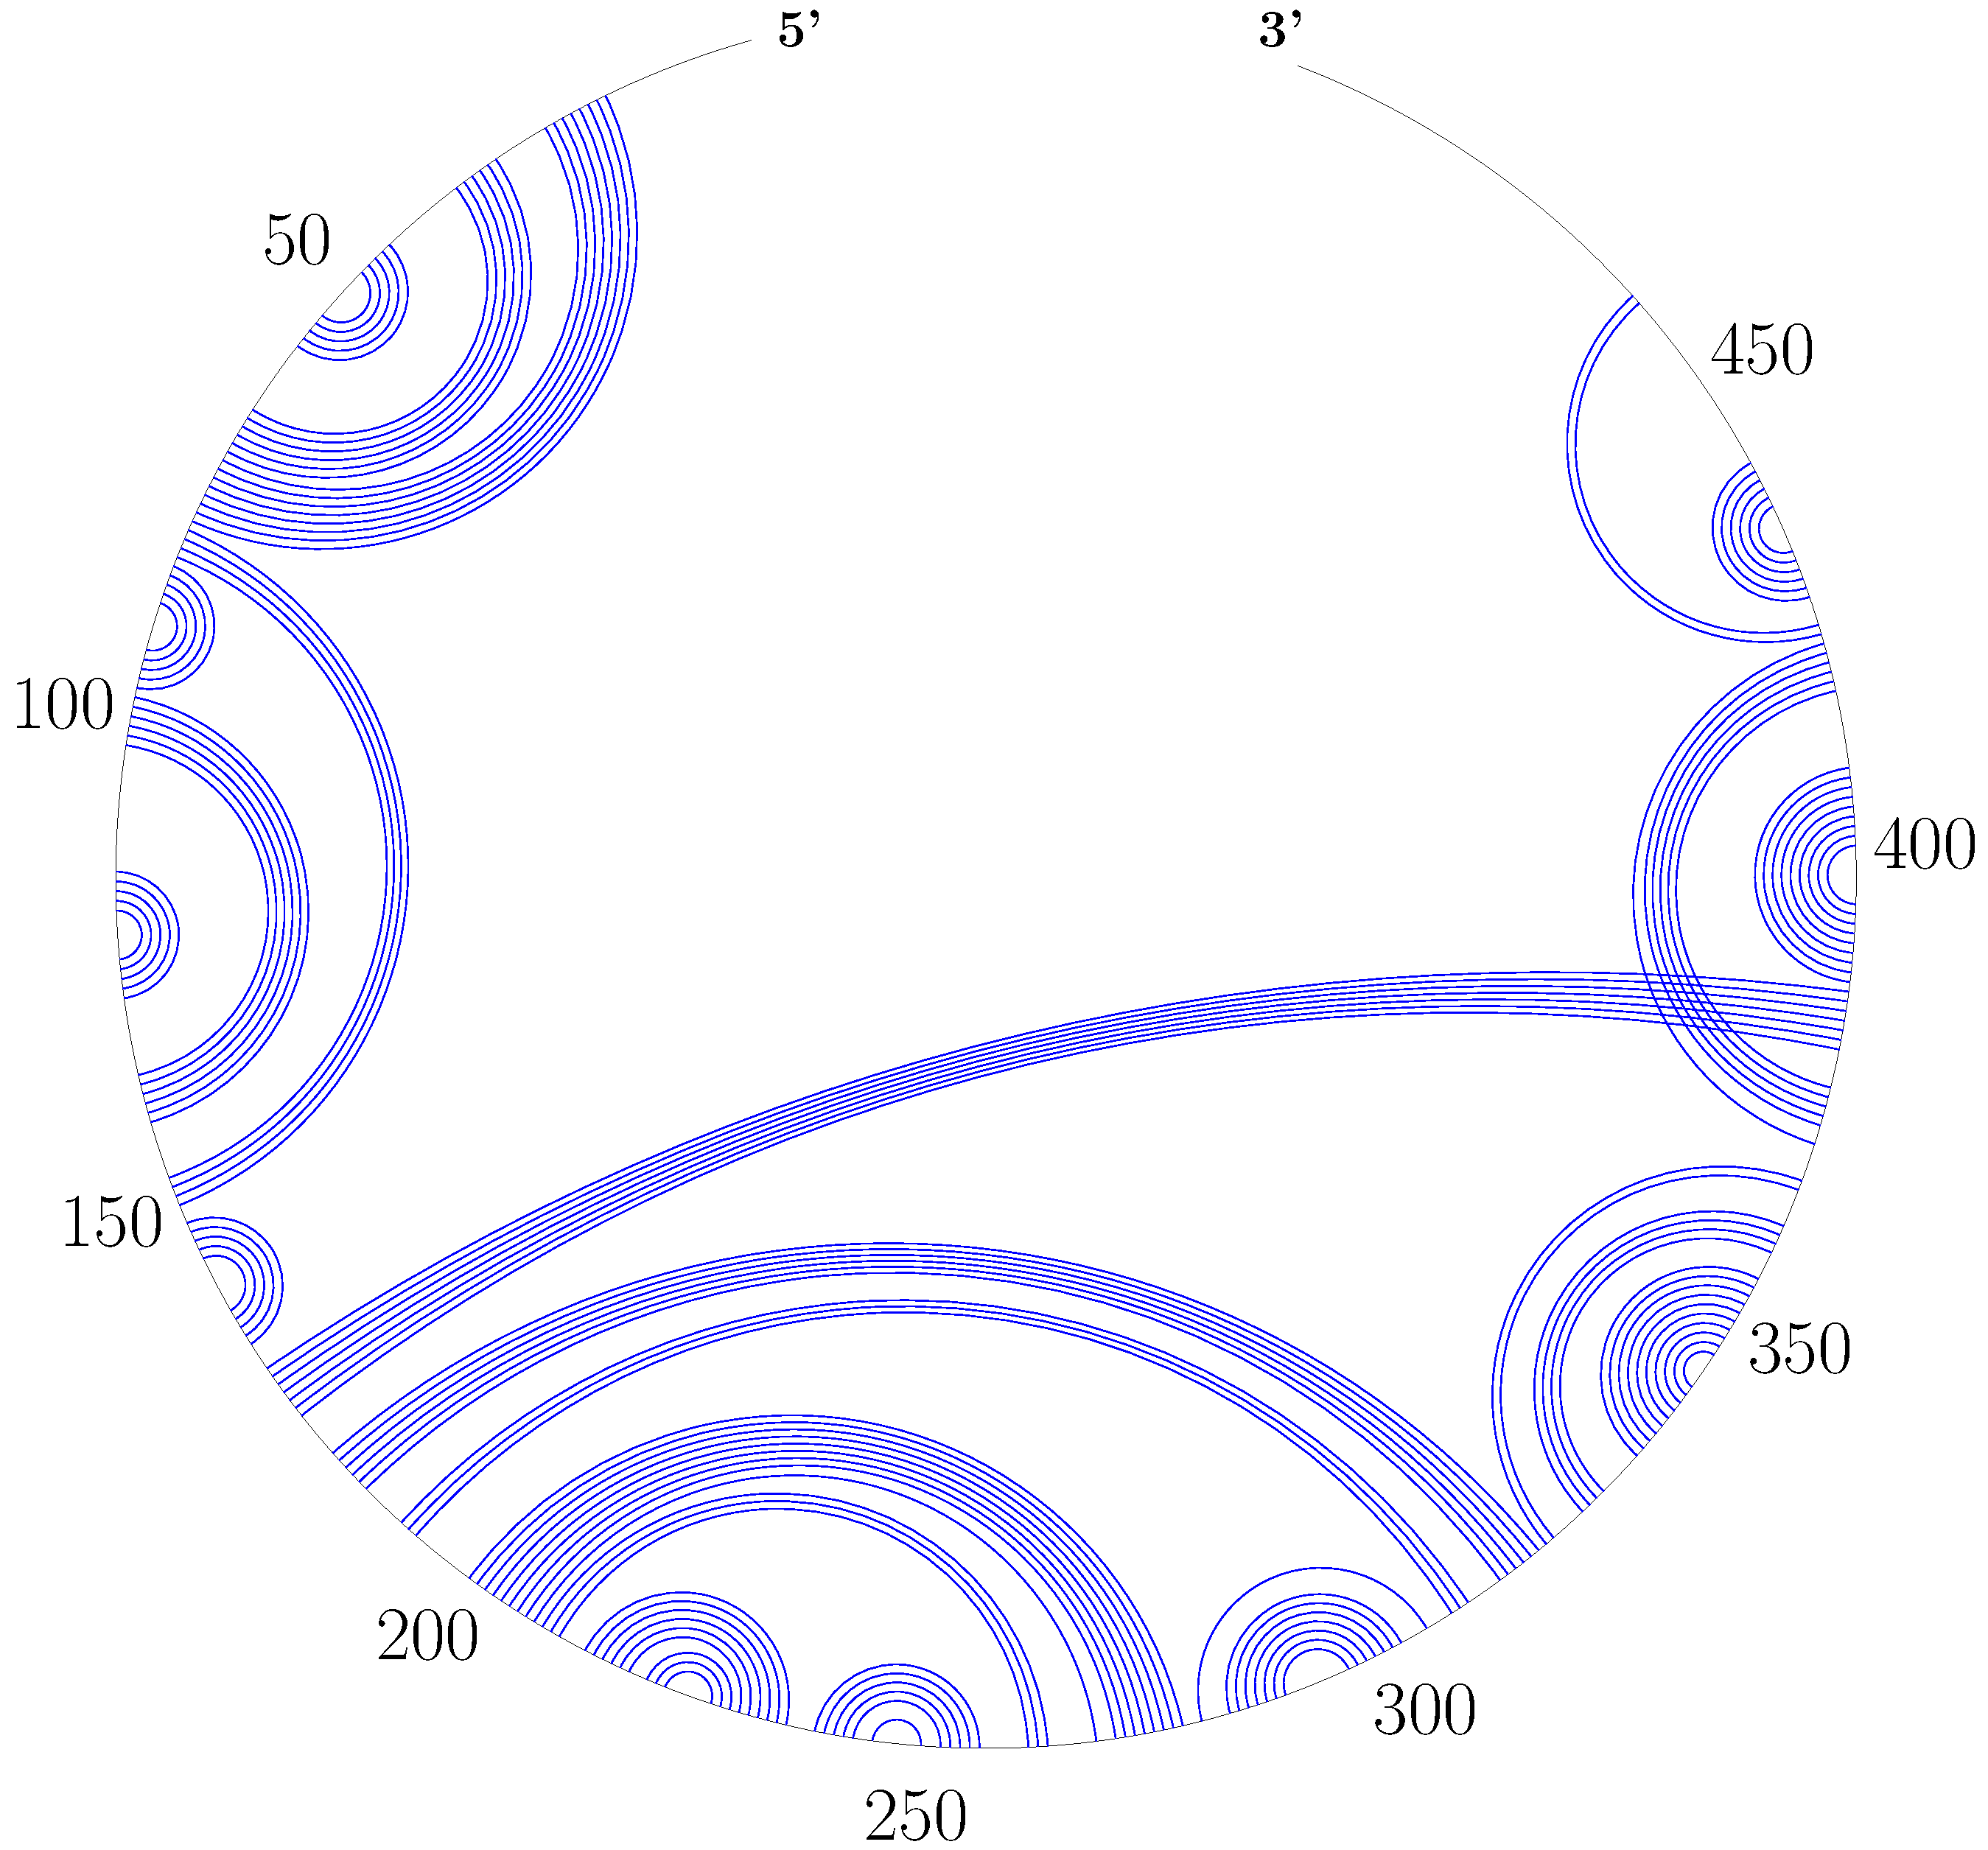
\includegraphics[width=0.22\textwidth]{figs/grp1_gold} &
\hspace{-0.35cm}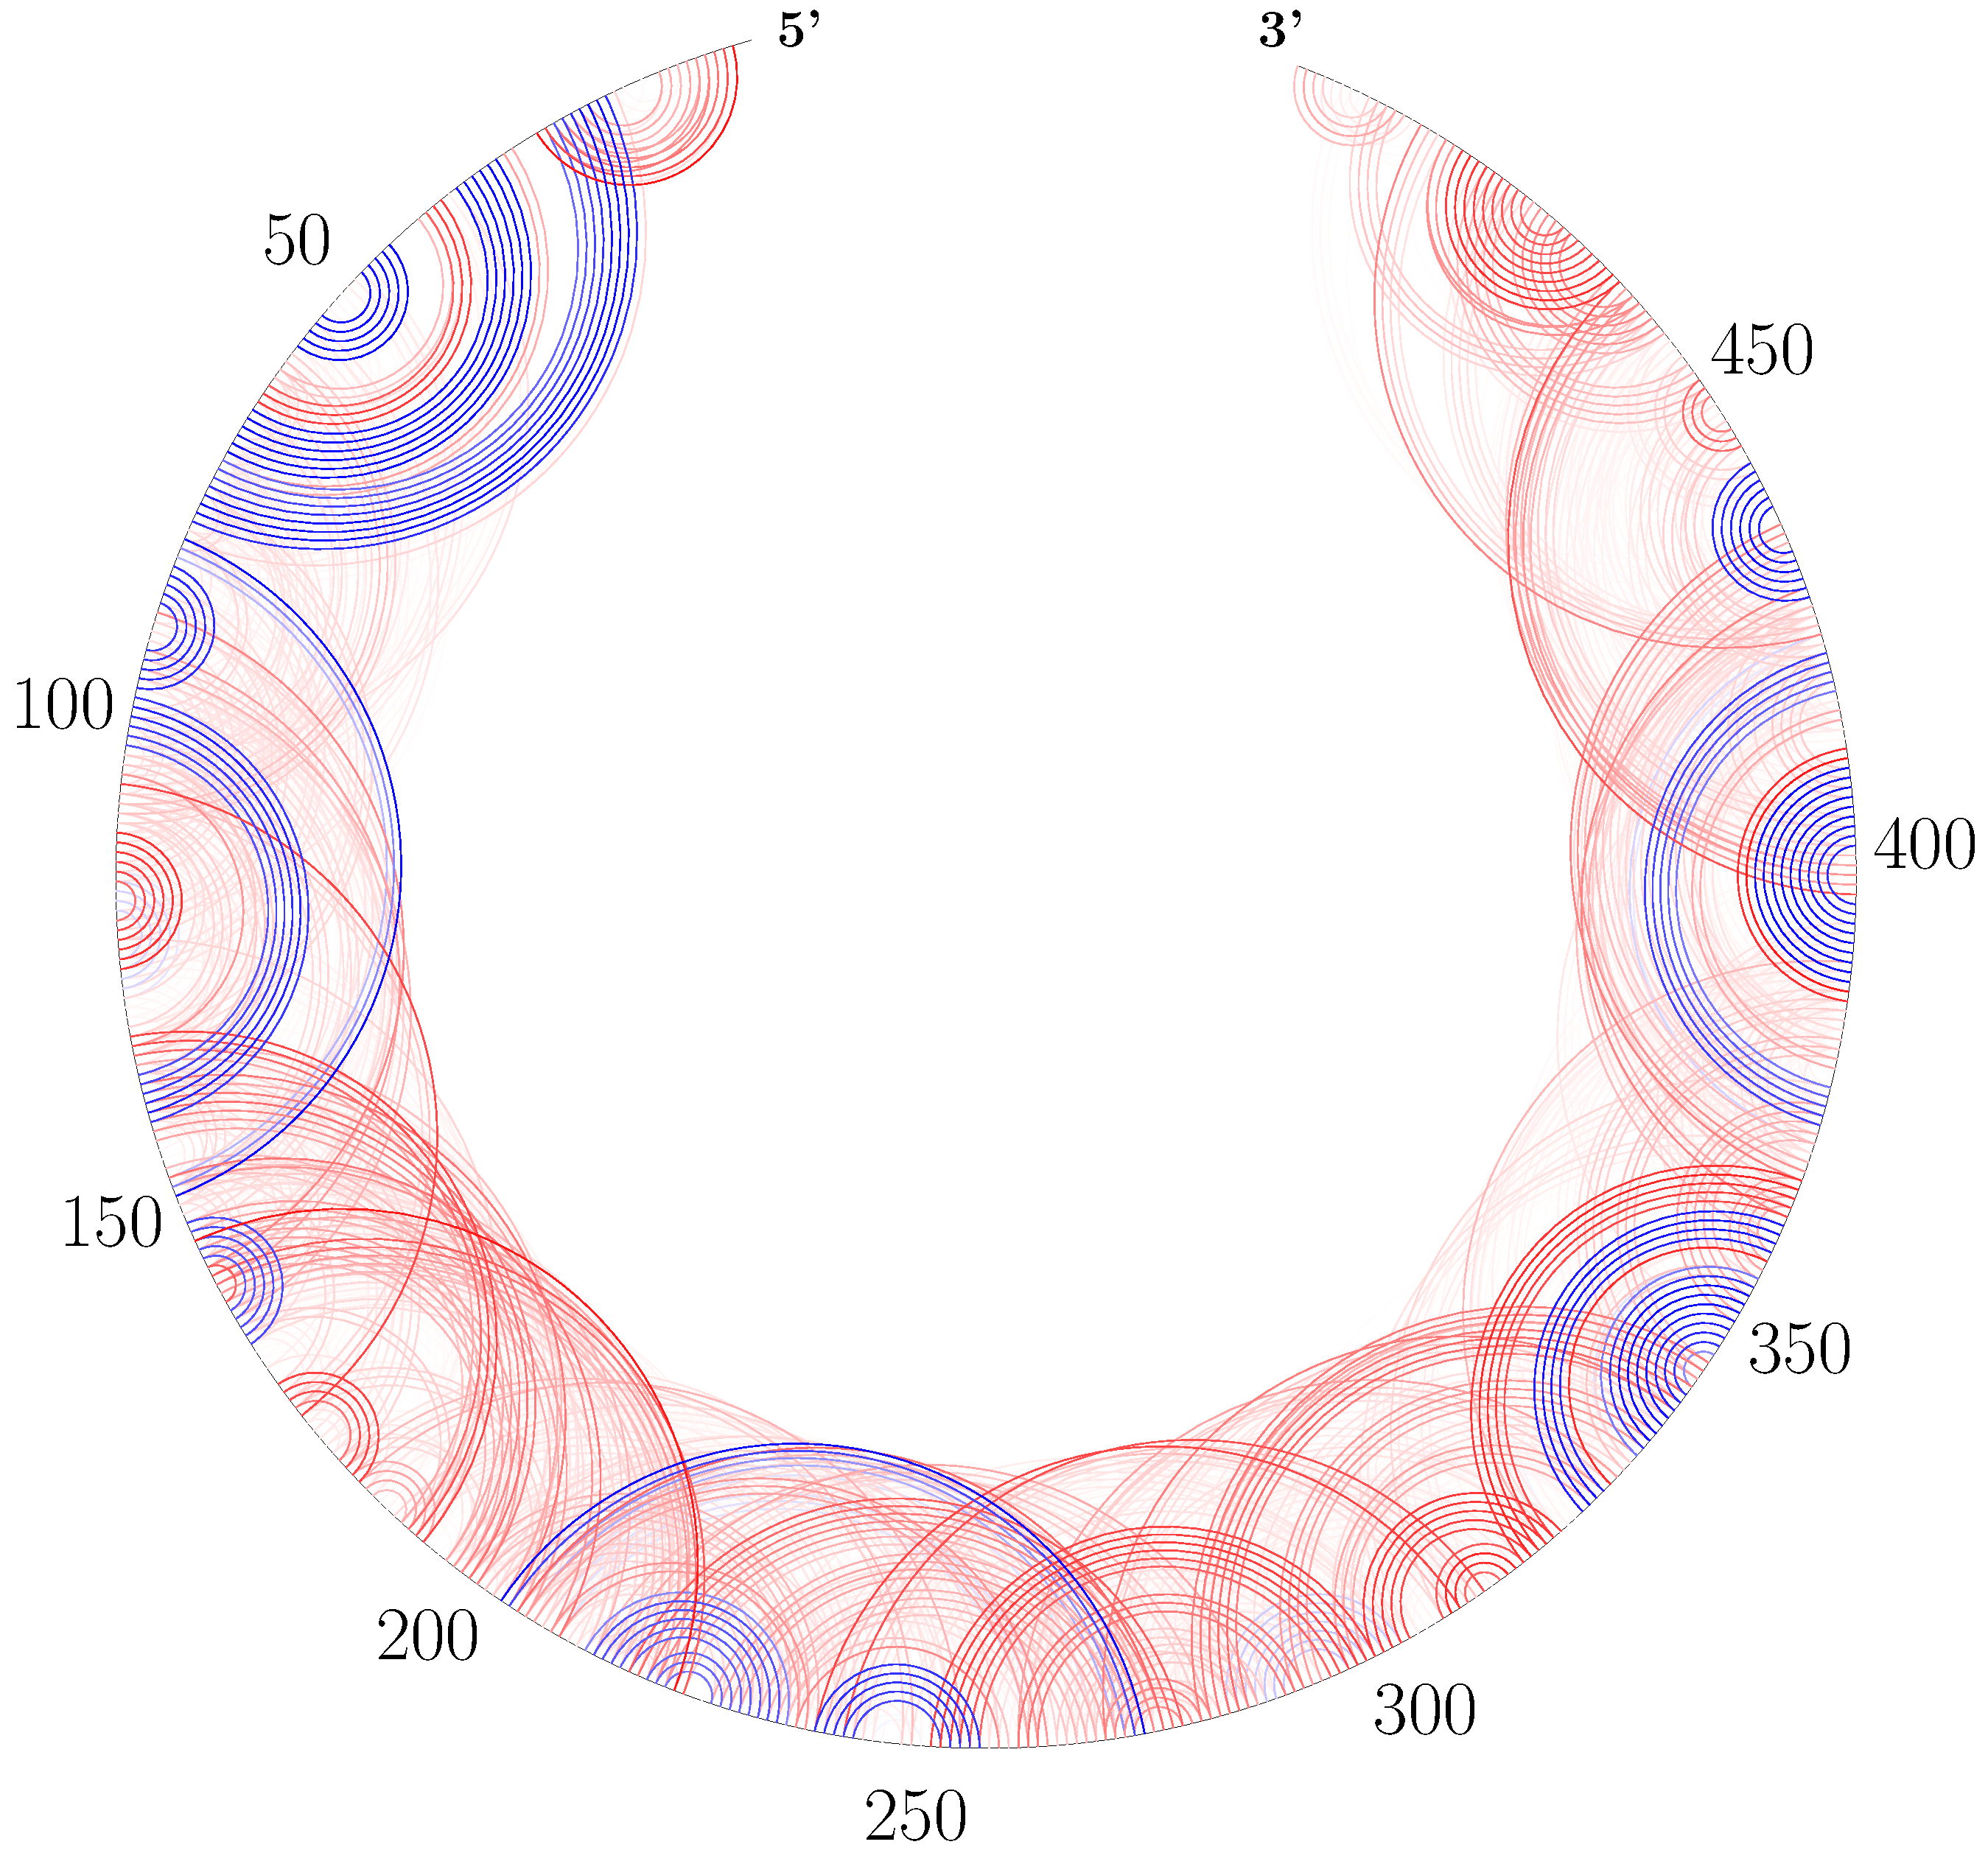
\includegraphics[width=0.22\textwidth]{figs/grp1_vienna_plfold_example.pdf} &
\hspace{-0.35cm}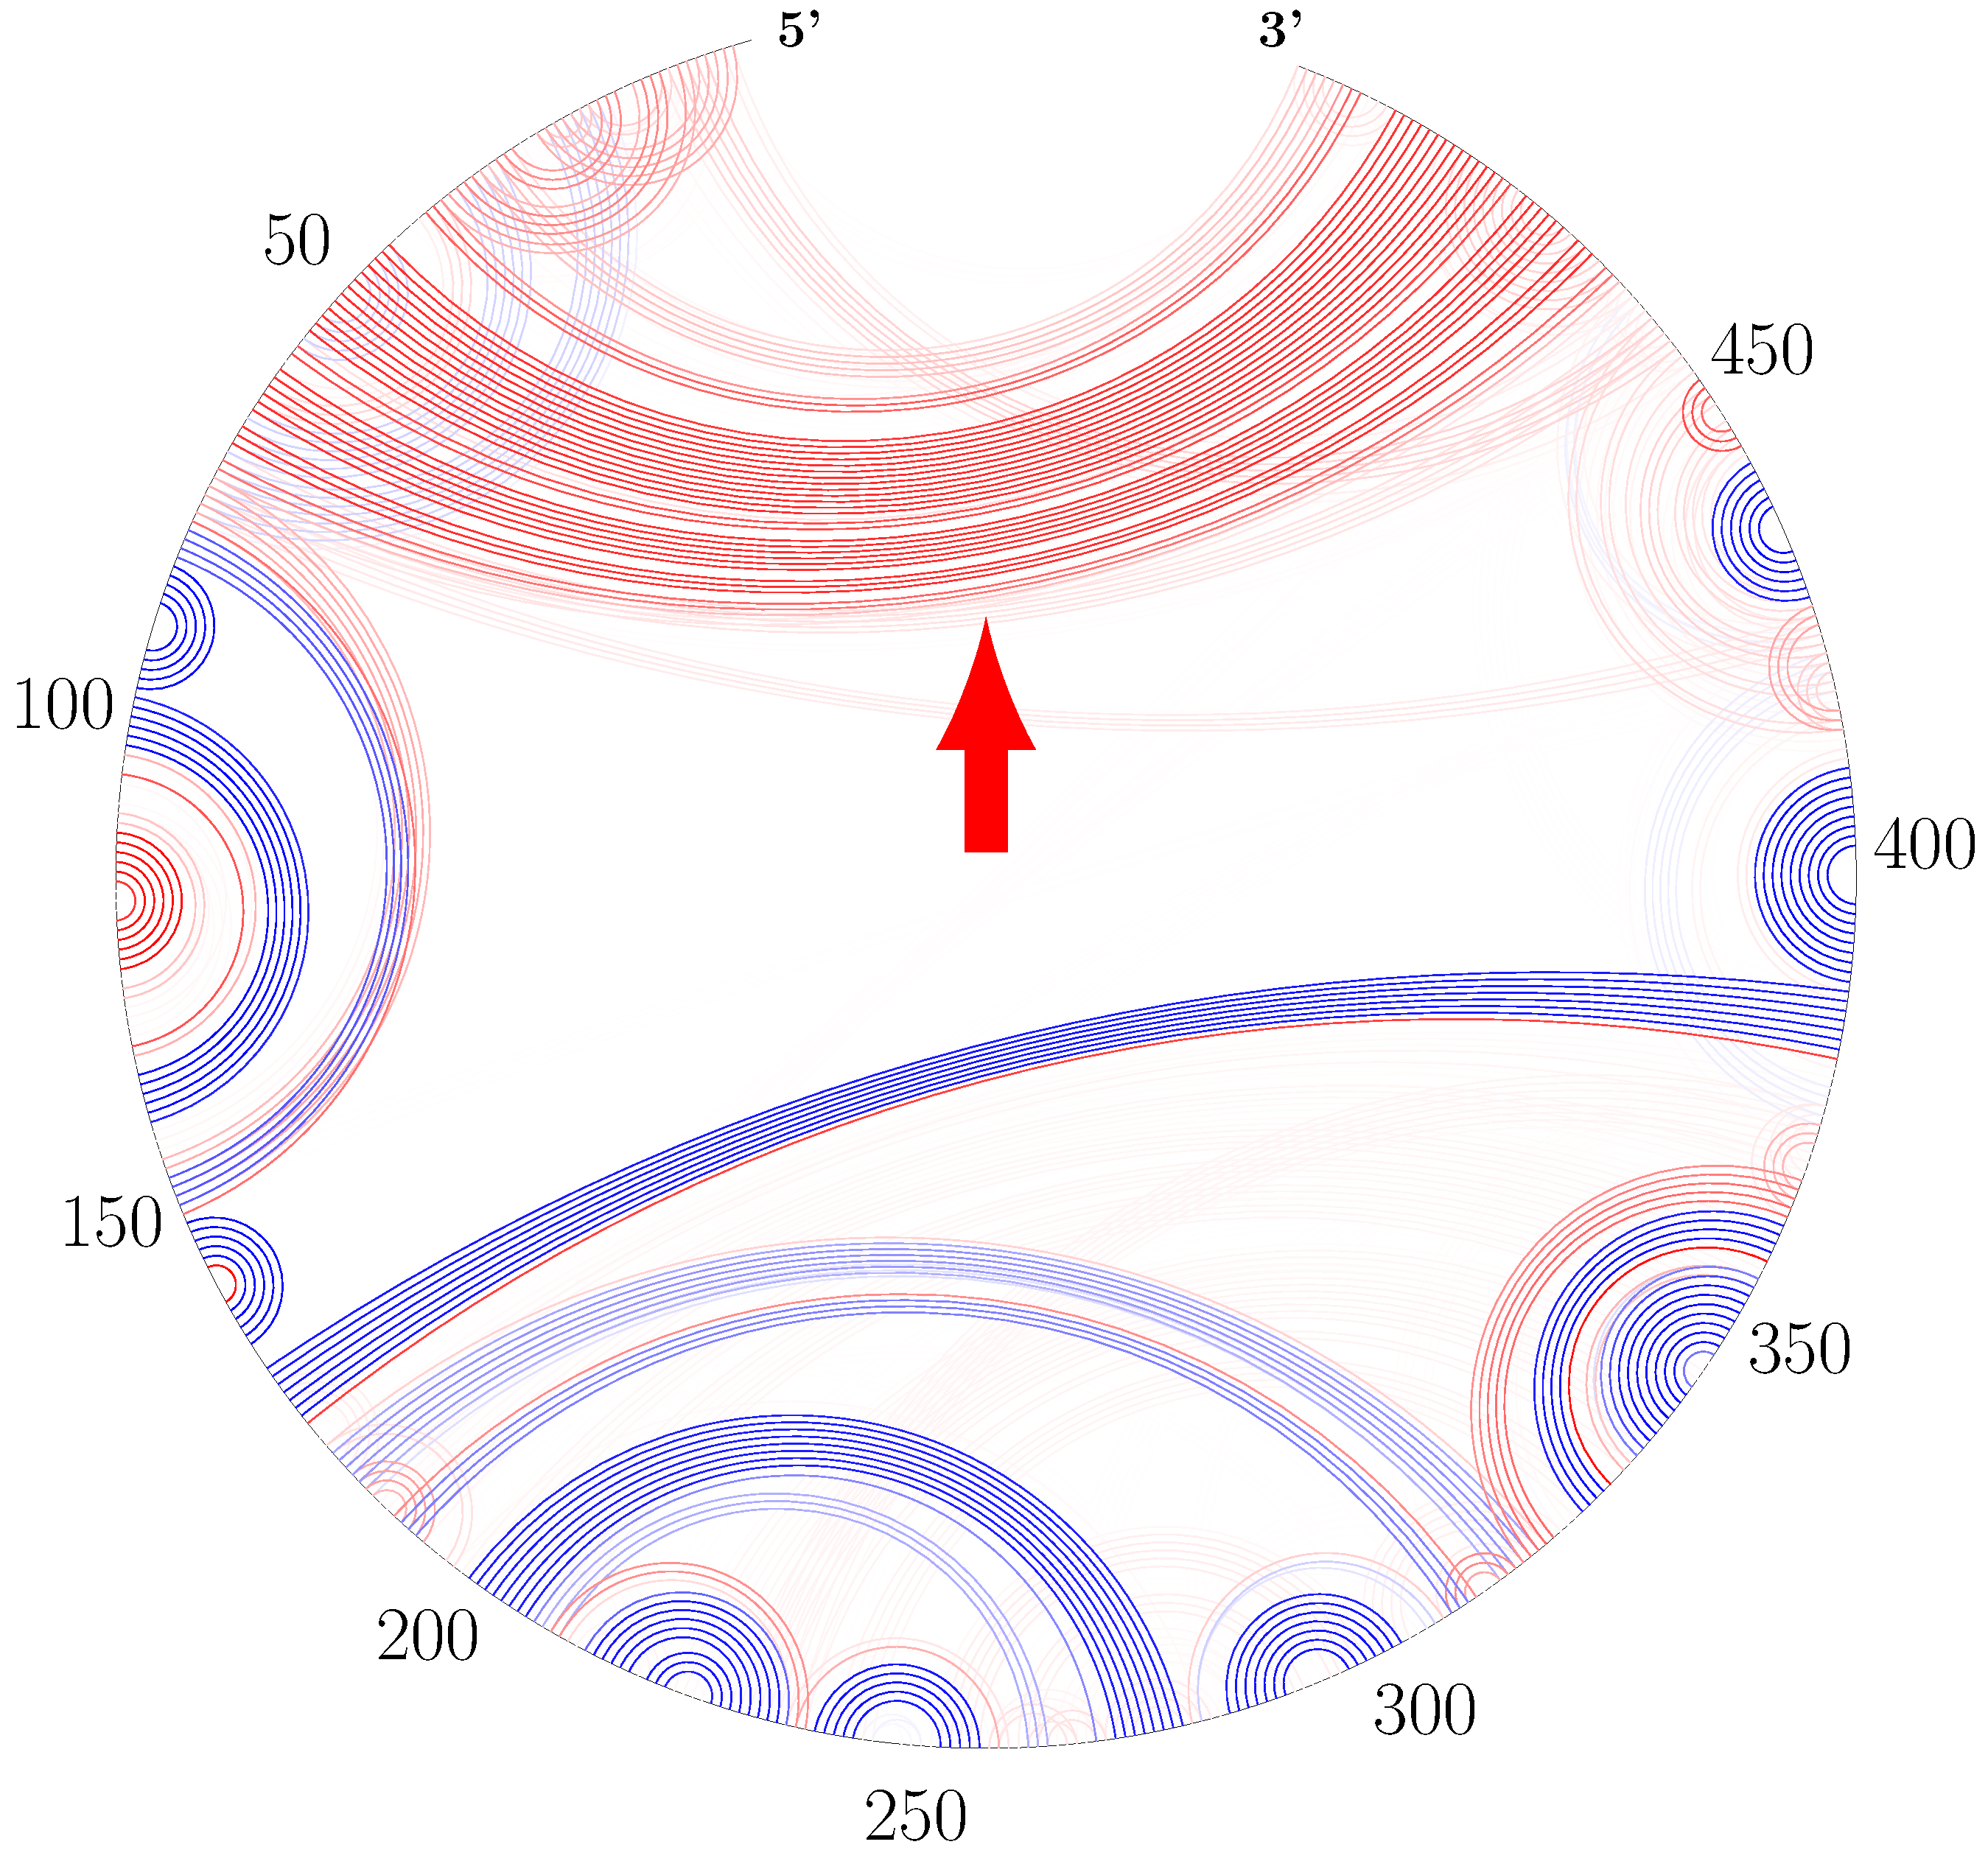
\includegraphics[width=0.22\textwidth]{figs/grp1_vienna_example} &
\hspace{-0.35cm}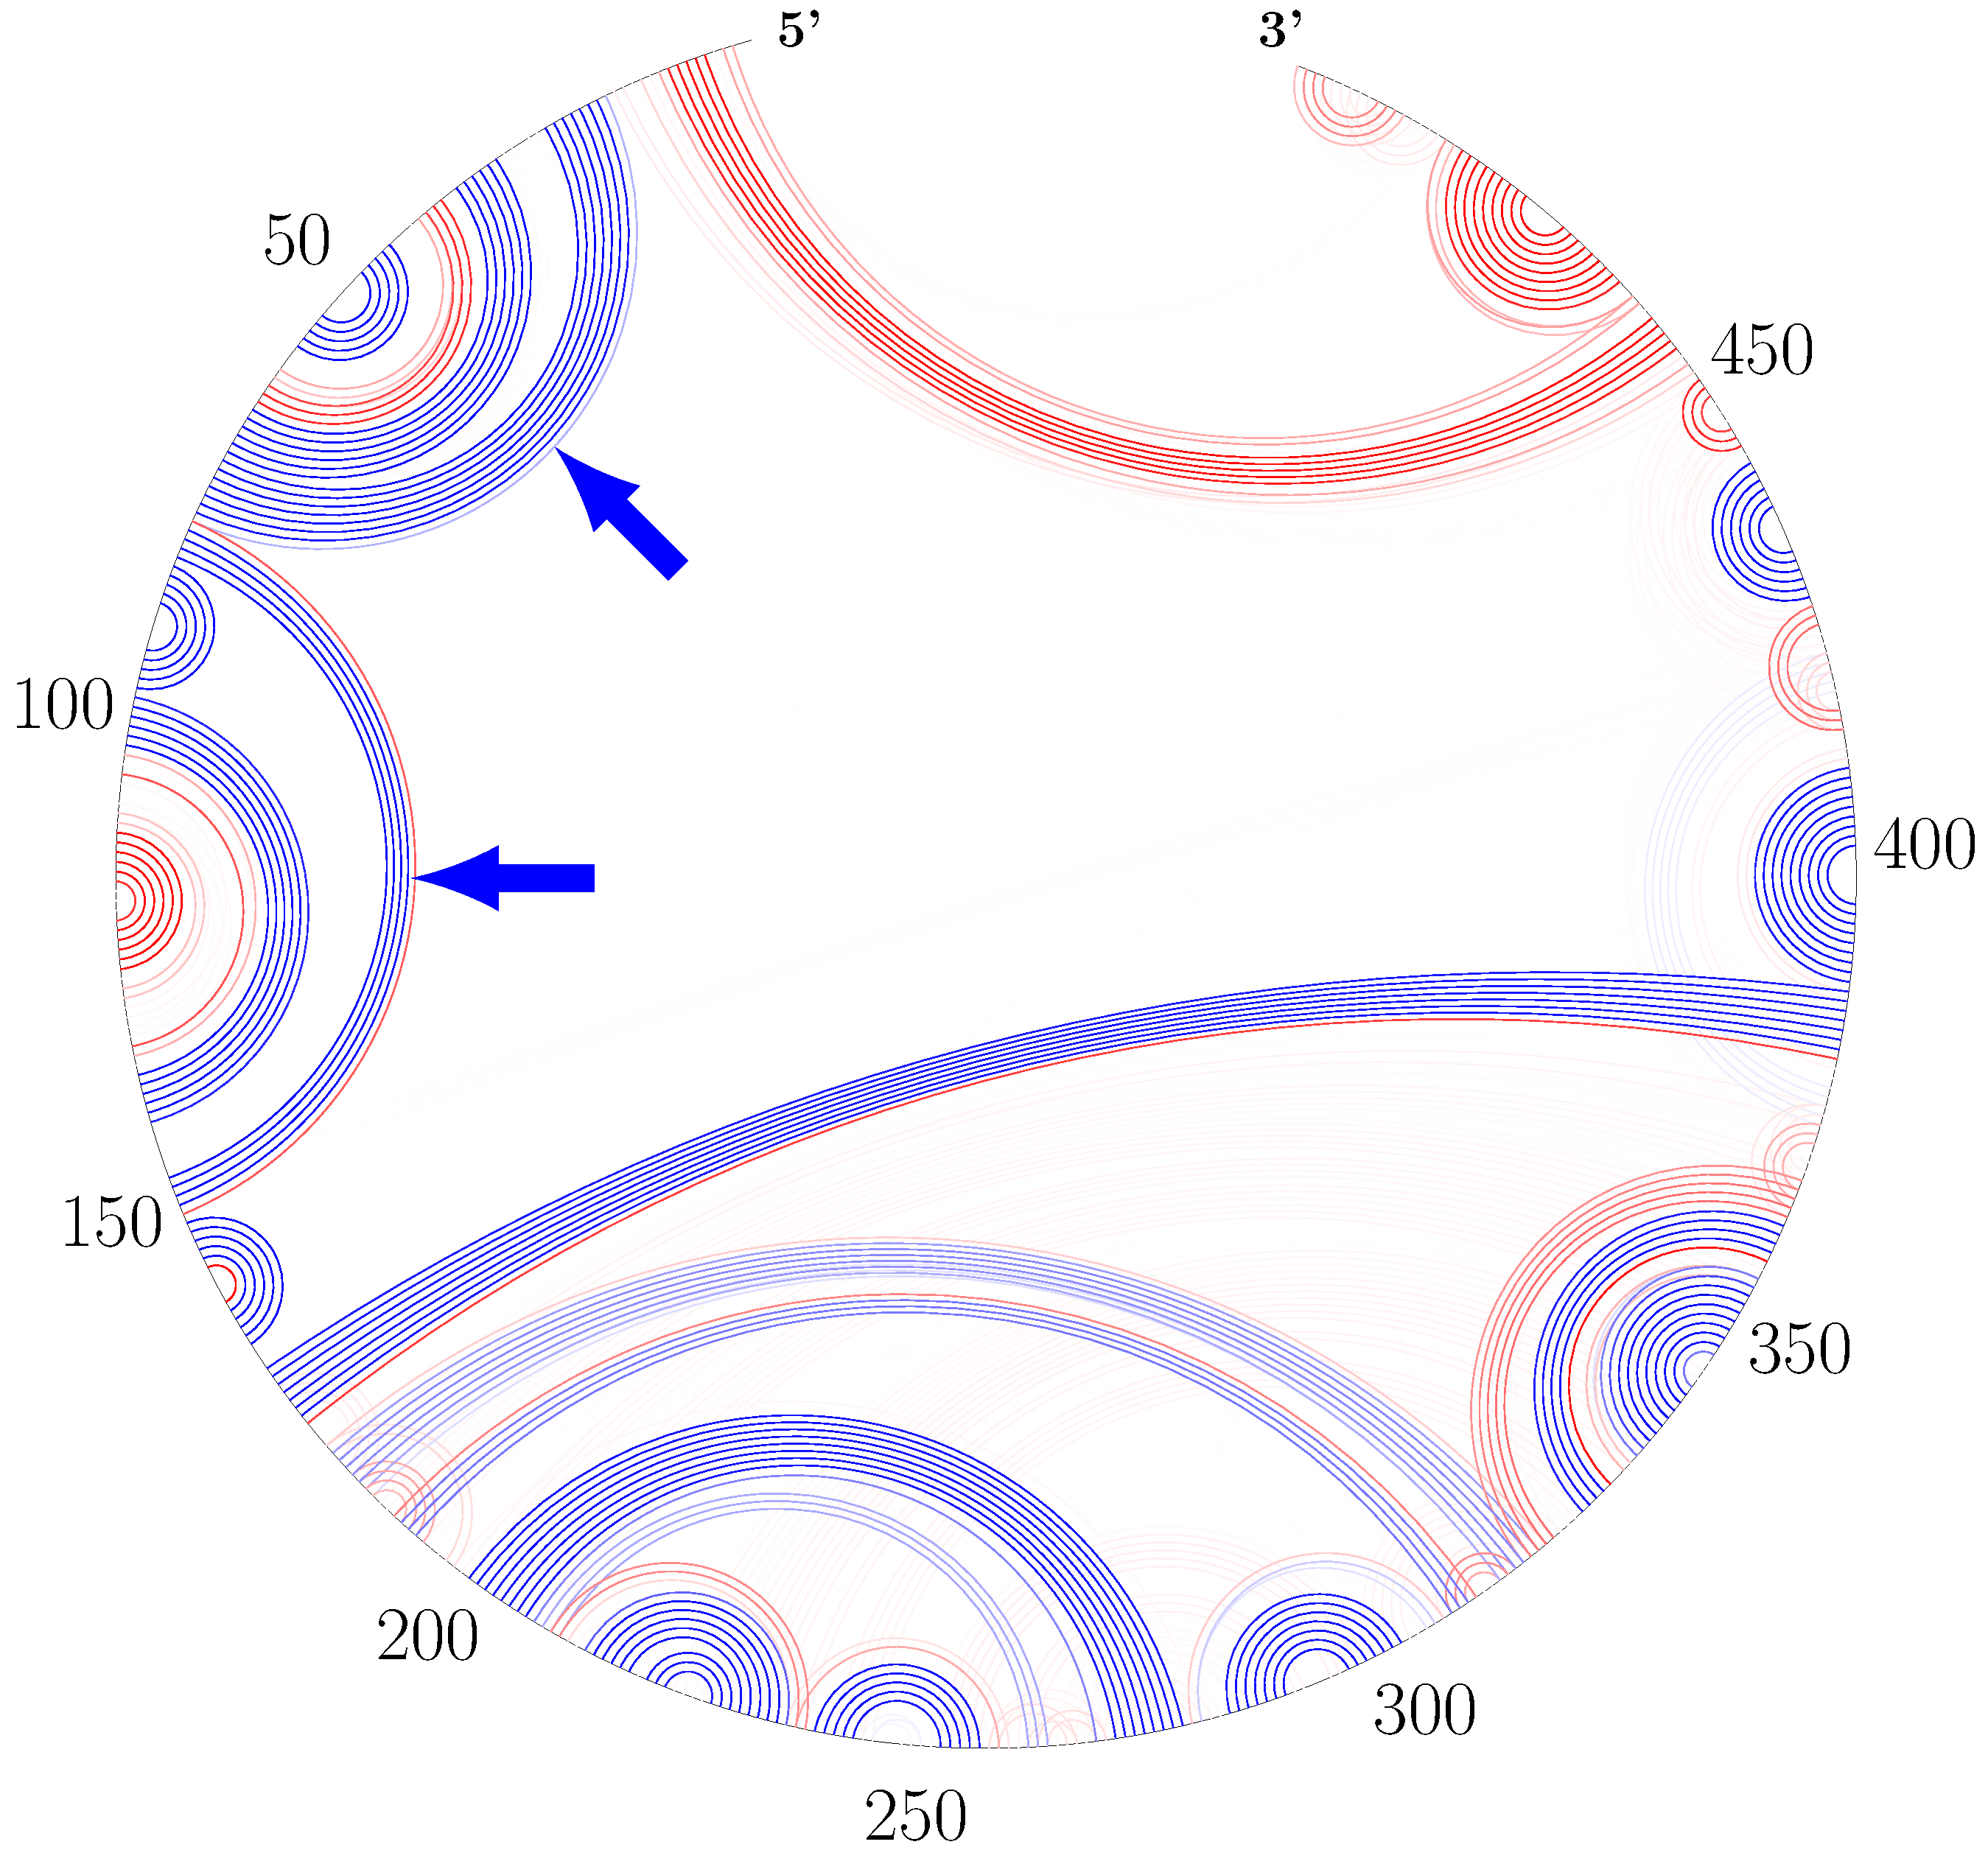
\includegraphics[width=0.22\textwidth]{figs/grp1_lpv_example.pdf}
\\[-0.2cm]
\end{tabular}
\caption{{\bf A}: Ensemble defect (expected number of incorrectly predicted nucleotides; lower is better) comparison between \viennarnafold and \linearpartition on the ArchiveII dataset.
  {\bf B}: Ensemble defect difference for each family.
  \linearpartition has lower ensemble defects for longer families:
   on average 56.3 less incorrectly predicted nucleotides on 23S rRNA and 8.3 less over all families.
  {\bf C--F}: An example of \ecoli 23S rRNA (shaded point in {\bf A}). 
  {\bf C}: Circular plot of the ground truth.
{\bf D--F}: Base pair probabilities from \viennarnaplfold (with default window size $70$), \rnafold and \linearpartition, respectively; 
Blue denotes pairs in the known structure and Red denotes predicted pairs not in the known structure.  
  The darkness of the line indicates pairing probability.
%  with the darkest lines close to a probability of 1. 
  {\bf G--J}: Circular plots of {\it C.~ellipsoidea} Group I Intron. 
%base pairs in the ground truth are in blue;
% blue and red indicate correct and incorrect base pairs,
% respectively, 
% and color darkness represents probabilities.
See Fig.~\ref{fig:example} 
% and~\ref{fig:circular_grp1} 
for another view of this example. % {\it C.~ellipsoidea} Group I Intron.
\label{fig:ensemble}
\vspace{-0.2cm}
}
\end{figure*}


Fig.~\ref{fig:runtime} compares the efficiency and scalability between the two baselines, 
\viennarnafold and \contrafold,
and our two versions, \linearpartitionv and \linearpartitionc.
% fair comparison, hack contrafold and vienna
To make the comparison fair, 
we disable the downstream tasks
(MEA prediction in \contrafold, and centroid prediction and visualization in \rnafold)
% which will be run together with partition function and base pairing probability calculation by default, 
which are by default enabled.
 % with partition function and base pairing probabilities calculation,
% for instance, 
%% These tasks are MEA structure generation in \contrafold,
%% as well as centroid structure generation and prediction visualization in \viennarnafold. 
Fig.~\ref{fig:runtime}A shows that both \linearpartitionv and \linearpartitionc
scale almost linearly with sequence length $n$.
The runtime deviation from exact linearity is due to the relatively short sequence lengths in the ArchiveII dataset, 
which contains a set of sequences with well-determined structures~\cite{sloma+mathews:2016}. 
%are relatively short
% (average length is 222.2~\nts).
Fig.~\ref{fig:runtime}A also confirms that the baselines scale cubically and the $O(n^3)$ runtimes are substantially slower than \linearpartition on long sequences. 
For the {\it H.~pylori} 23S rRNA sequence (2,968~\nts, the longest in ArchiveII), 
both versions of \linearpartition  take only 6 seconds,
while \rnafold and \contrafold take 73 and 120 seconds, resp.
%and  almost 120 seconds.


% Fig.~\ref{fig:runtime}B visualizes the runtimes on RNAcentral sampled sequences.
% We set the runtime limit for a sequence to be at most 24 hours.
We also notice that both \rnafold and \contrafold have limitations on even longer sequences.
% although \viennarnafold designs a scalar estimated from minimum free energy of the given sequence to avoid overflow, 
\rnafold scales the magnitude of the partition function 
using a constant estimated from the minimum free energy of the given sequence to avoid overflow,
% but is still easy to get overflow 
but overflows still occur 
on long sequences.
For example, it overflows %on partition function calculation 
on the 19,071~\nts sequence in the sampled RNAcentral dataset.
% so we only show the runtime before this sequence for \viennarnafold.
% Unlike \viennarnafold, \linearpartition adopts a log space partition function calculation
% as \contrafold and solve overflow issue fundamentally.
% \contrafold adopts logarithmic scale of partition function to solve overflow issue,
% but it cannot run on sequence longer than 32,753~\nts due to memory limitation. 
\contrafold stores the logarithm of the partition function to solve the overflow issue,
but cannot run on sequences longer than 32,767~\nts due to using {\tt unsigned short}
% in its implementation
to index sequence positions.
% Beyond these limitations, 
\linearpartition, like \contrafold, performs computations in the log-space,
but can run on all sequences in the RNAcentral dataset.
Fig.~\ref{fig:runtime}B compares the runtime of four systems on a sampled subset of RNAcentral dataset,
and shows that % only \linearpartition can finish all the examples,
on longer sequences the runtime of \linearpartition is exactly linear.
% but \viennarnafold only runs on the first 17 data points because of overflow issue. 
%Comparing the runtimes of
For the 15,780~\nts sequence, 
 % \viennarnafold can run,
the longest example shown for \rnafold, % in Fig.~\ref{fig:runtime}B,
%\viennarnafold takes more than 3 hours and
\linearpartitionv is 256$\times$ faster (more than 3 hours vs.~44.1 seconds). 
Note that \rnafold may not overflow on some longer sequences, 
where \linearpartitionv should enjoy an even more salient speedup.
% ???\contrafold stops at 17th or need to continue???
For the longest sequence that \contrafold can run (32,753~\nts) in the dataset,
\linearpartition is 2,771$\times$ faster (2.5 days vs.~1.3 min.).
%% % is 22,911~\nts, 
%% it takes 60.7 hours,
%% compared to \linearpartitionc's 52.4 seconds
%% (2,771$\times$ speedup).
% 32,767
% We find \contrafold has a sequence length limitation of 32,767~\nts due to using "unsigned short" in its implementation.
% We also test on an artificial sequence with length of 32,767~\nts, 
% the upper limit for \contrafold, 
% and the runtime is ?????
Even for the longest sequence in RNAcentral
(Homo Sapiens Transcript NONHSAT168677.1 with length 244,296~\nts~\cite{Zhao+:2016}),
both \linearpartition versions finish in $\sim$10 minutes.

Fig.~\ref{fig:runtime}C
%% compares the memory usage 
%% %of 4 systems 
%% on RNAcentral-sampled sequences. 
%% It 
shows that  \rnafold and \contrafold use $O(n^2)$ space
while \linearpartition uses $O(n)$.
%% With increasing length, the two baselines require much more memory space than \linearpartition.


%%%%%%%%%%%%%%%%

%%%%%%%%%%%%%%%%%




%\smallskip
Now that we have established the speed of  \linearpartition,
%in the next two subsections,
we move on to the quality of its output.
%i.e., the resulting Boltzmann distribution and base pairing probabilities.
%% We first study the correlation with ground truth structures in Sec.~\ref{sec:corr},
%% and then use base pairing probabilities for downstream structure predictions in Sec.~\ref{sec:acc}.

\vspace{-.1cm}
\subsection{Correlation with Ground Truth Structures}
\label{sec:corr}

% ensemble defect


We use {\em ensemble defect}~\cite{Zadeh+:2010} (Fig.~\ref{fig:ensemble}A--B)
to represent the quality of the Boltzmann distribution.
It is the expected number of incorrectly predicted nucleotides over the whole ensemble at equilibrium,
and formally,
for a sequence \vecx and its ground-truth structure \vecystar, the ensemble defect is% $\Phi(\vecx,\vecystar)$ %denotes the average number of incorrectly paired nucleotides at equilibrium, and is formalized as:
\begin{equation}
%\begin{split}
\vspace{-0.2cm}
\Phi(\vecx,\vecystar) = \sum_{\vecy \in \mathcal{Y}(\vecx)} p(\vecy) \cdot d(\vecy, \vecystar) % \\ 
%                 &= |\vecx| - 2 \sum_{(i,j) \in \mathrm{pairs(\vecystar)}} p_{i,j} - \sum_{j \in \mathrm{unpaired(\vecystar)}} q_{j}
%\end{split}
\label{eq:phi}
\end{equation}
where % $\phi$ is the folding model, 
%  $\vecystar$ is the groud truth secondary structure, 
%  $\mathcal{Y(\vecx)}$ is the ensemble of the sequence $\vecx$, 
%  and $|\vecx|$ is the sequence length. % ($N+1$ is for conveniently describing unpaired bases);
$p(\vecy)$ %=e^{-\frac{\Delta G^\circ(\vecy)}{RT}} / Q(\vecx)$
is the probability of structure \vecy % of the structure $\vecy$ in the ensemble.
in the ensemble %among all possible structures
$\mathcal{Y(\vecx)}$,
and $d(\vecy, \vecystar)$ is the distance between $\vecy$ and $\vecystar$, %,  defined as:
defined as the number of incorrectly predicted nucleotides in \vecy:
\vspace{-0.3cm}
 \[% \begin{equation*}
  \begin{split}
    d(\vecy,\vecystar)=  |\vecx|  & - |\pairs(\vecy) \cap \pairs(\vecystar)|\\
                        & - |\unpaired(\vecy) \cap\unpaired(\vecystar)|
  \end{split}
%  \label{eq:d}
 \]% \end{equation*}
 % \vspace{-0.2cm}
%% where  $\pairs(\vecystar)$ is the set of base pairs in $\vecystar$,
%% and $\unpaired(\vecystar)$ is the set of unpaired bases in $\vecystar$.
 The na\"ive calculation of Eq.~\ref{eq:phi} requires enumerating all possible % (exponentially many)
 structures in the ensemble, % which is intractable,
  but by plugging $d(\vecy, \vecystar)$ %Eq.~\ref{eq:d}
  into Eq.~\ref{eq:phi} % and with some derivations,
  we have~\cite{Zadeh+:2010}
\begin{equation}
\vspace{-0.2cm}
\begin{split}
\Phi(\vecx,\vecystar) = |\vecx| - 2\!\! \sum_{(i,j) \in \pairs(\vecystar)} p_{i,j} - \sum_{j \in \unpaired(\vecystar)} q_{j} \notag
\end{split}
\label{eq:phi2}
\vspace{-0.2cm}
\end{equation}
where $p_{i,j}$ is the probability of $i$ pairing with $j$ %, i.e., %(or the probability of $i$ being unpaired when $j=N+1$).
%% \(%[
%% p_{i,j} = \sum_{(i,j)\in \pairs(\vecy)} p(\vecy),
%% \)
and $q_{j}$ is the probability of $j$ being unpaired, i.e., $q_j = 1- \sum p_{i,j}$.
  % $S_{i,j}(s)$ is the a structure matrix with entries $S_{i,j}(s) \in \{0, 1\}$, i.e., if structure $s$ contains pair $(i,j)$, then $S_{i,j}(s) = 1$, otherwise $S_{i,j}(s) = 0$.
This means we can now use base pairing probabilities to compute the ensemble defect.

%  $d(\vecy, \vecystar)$ is the distance between $\vecy$ and $\vecystar$,  defined as:

\begin{figure}[!t]
  % \hspace{1.5cm}
\center
% \begin{tabular}{c|c|c|c}
\definecolor{darkgreen}{rgb}{0, 0.5, 0}
\newcommand{\bluetri}{{\color{blue} $\blacktriangle$}}
\newcommand{\greentri}{{\color{darkgreen} $\blacktriangle$}}
\newcommand{\redtri}{{\color{red} $\blacktriangle$}}
\newcommand{\bluecir}{{\color{blue} $\circ$}}
\newcommand{\greencir}{{\color{darkgreen} $\circ$}}
\newcommand{\redcir}{{\color{red} $\circ$}}
\begin{tabular}{cc}
\panel{A} & \hspace{-1cm}\panel{B} \\[-.7cm]
% \raisebox{8.7cm}{\hspace{-0.2cm}} %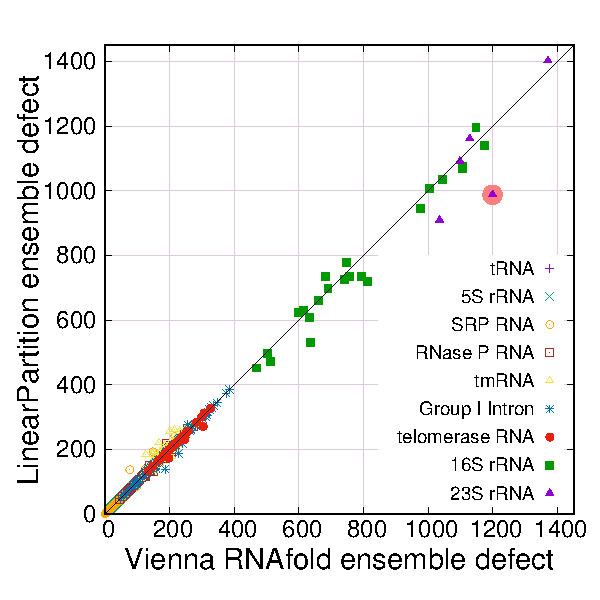
\includegraphics[width=0.4\textwidth]{figs/ensemble_defect} }
% &
% \hspace{-.2cm}\panel{A} & \hspace{-0.6cm}\panel{B} \\[-1cm] %& \hspace{-2.5cm}\panel{D}
	\multicolumn{2}{c}{
	  \hspace{-.3cm}
%          \vspace{-.2cm}
	  \raisebox{7.5cm}
	  {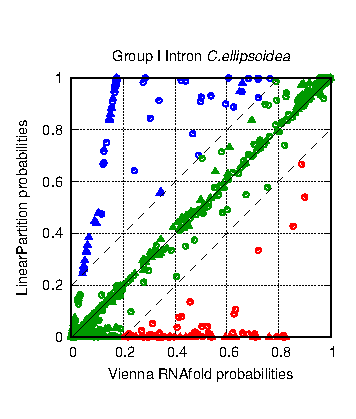
\includegraphics[width=4.4cm]{figs/prob_xy_grp1}}
	  \hspace{-4.5cm}
	   %\raisebox{0cm}
	  {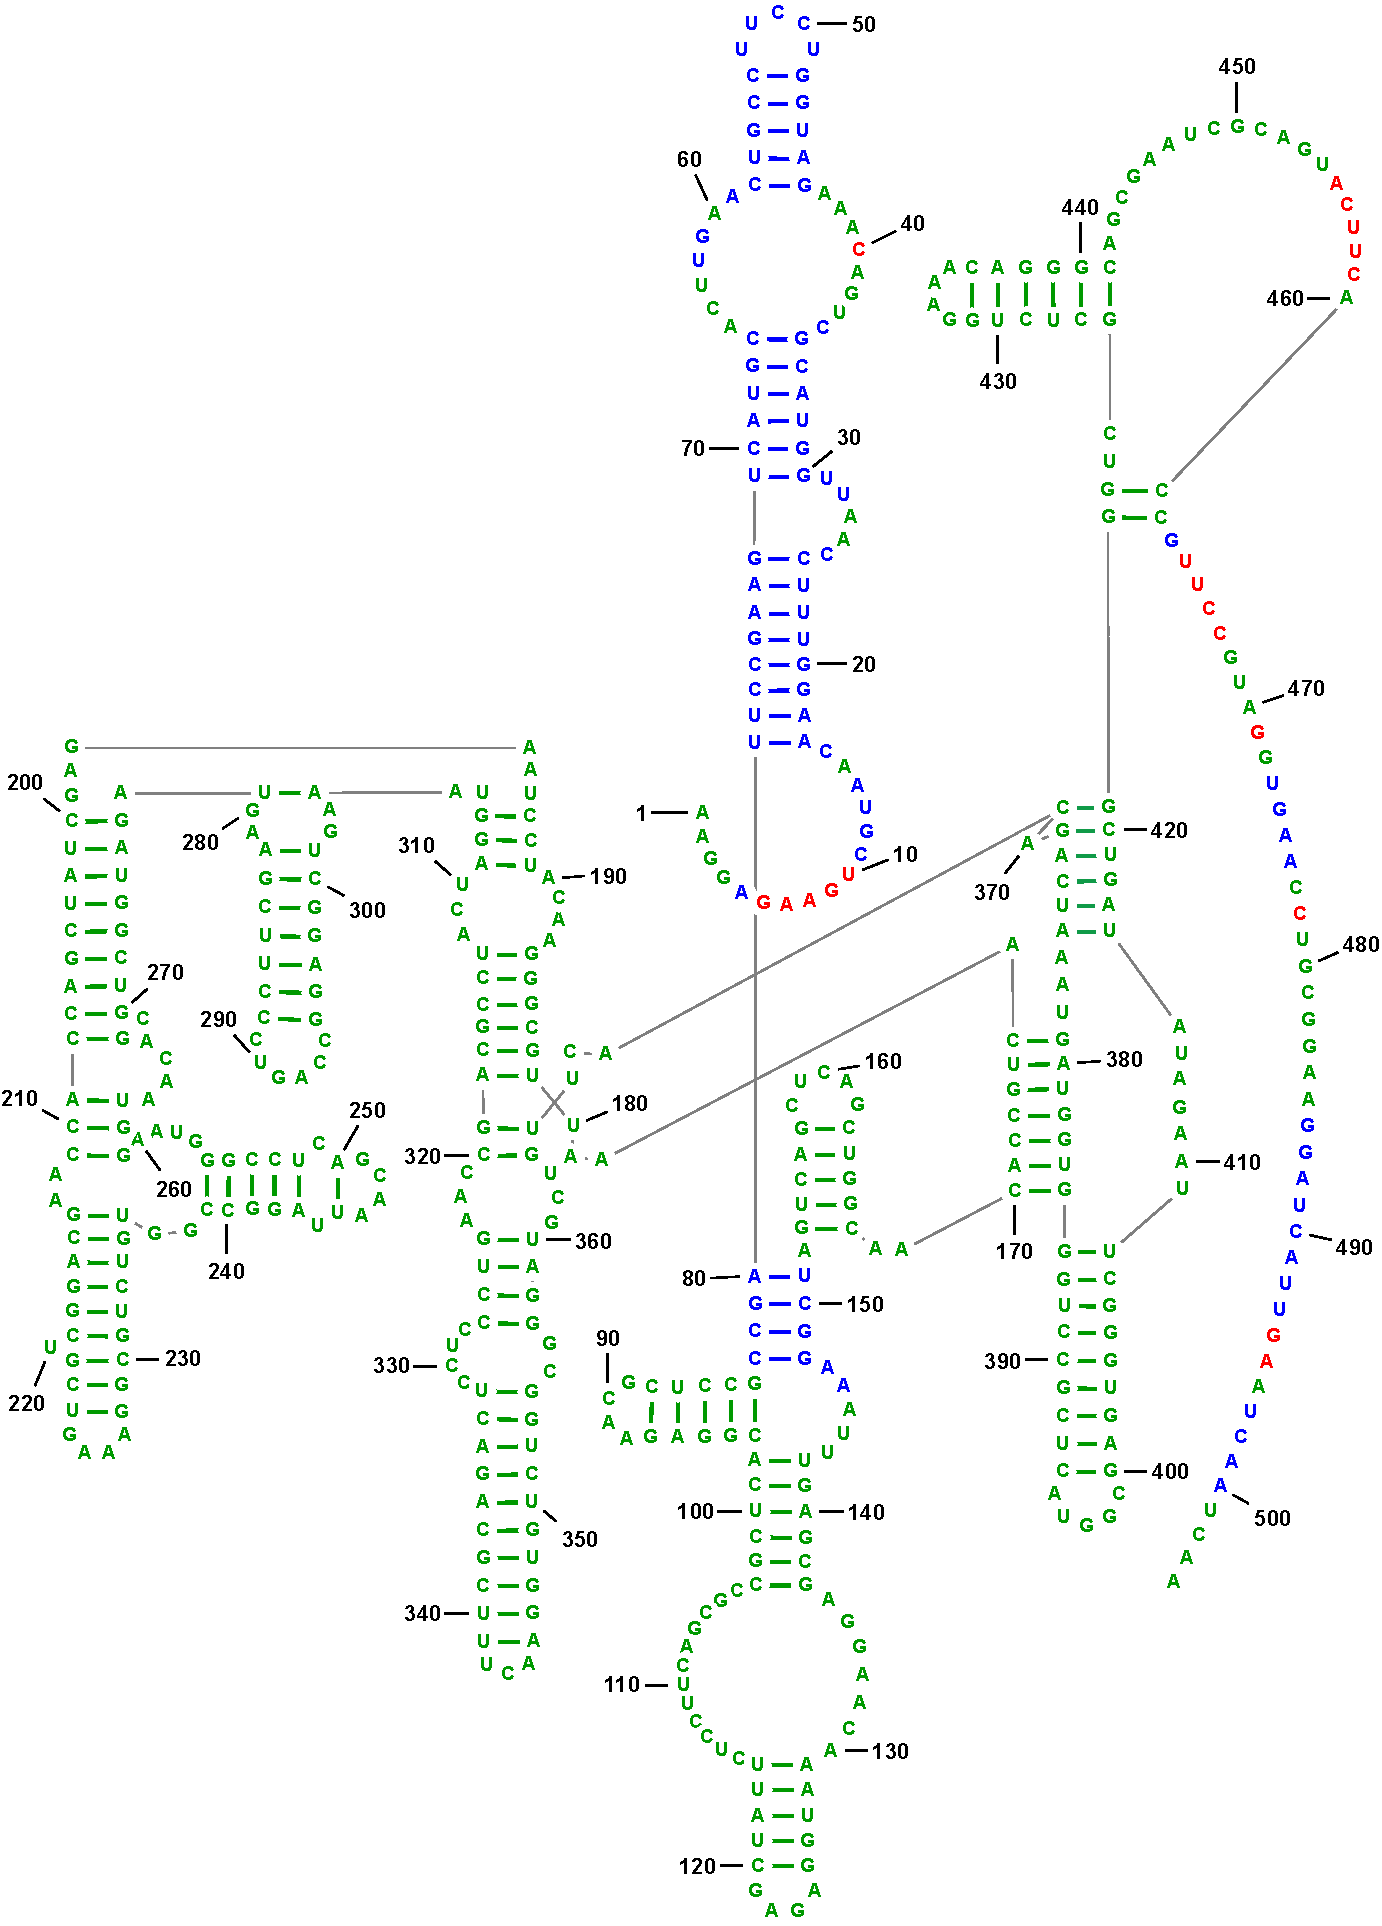
\includegraphics[width=0.5\textwidth]{figs/grp1_70_gutell_modified_2020}}
  	} \\[-1.6cm]
  	\hspace{-.0cm}\panel{C} &  \\[-1.cm]
  	\end{tabular}
% \hspace{-7cm}\panel{B} &\\[-.8cm]

% &&\raisebox{0cm}{\hspace{0.2cm}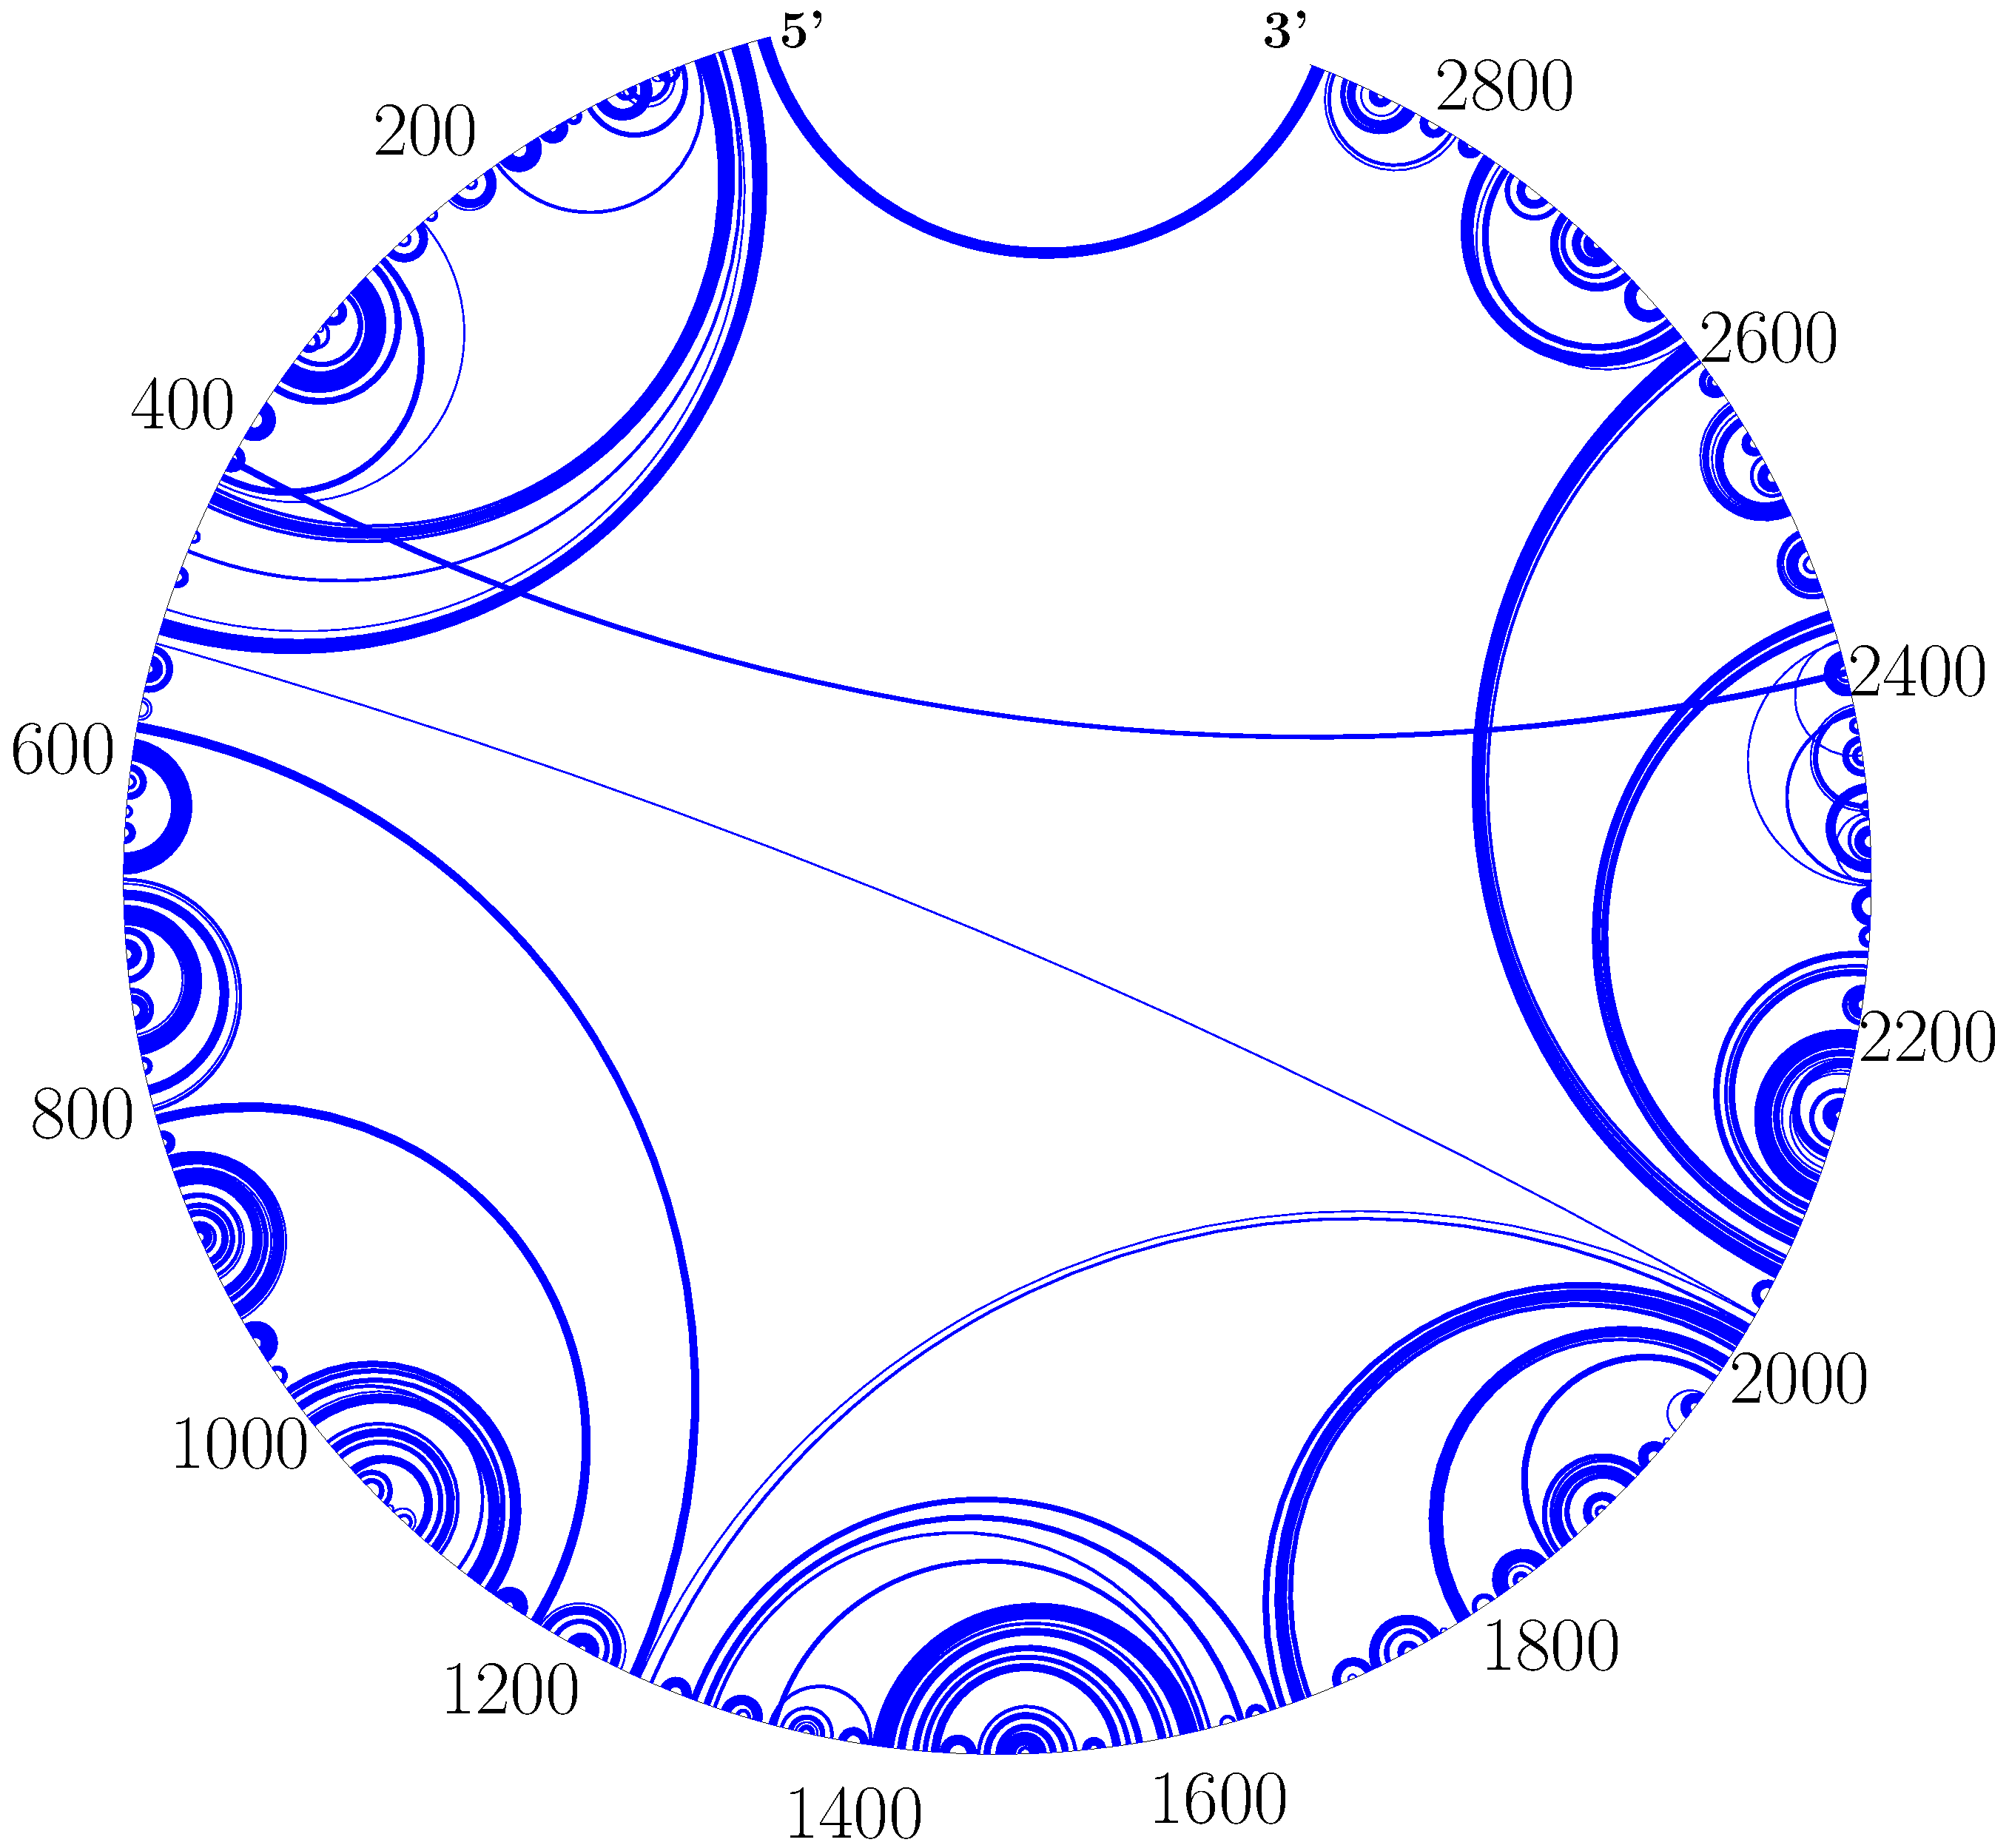
\includegraphics[width=0.25\textwidth]{figs/23s_gold}} \\
% &&\hspace{-4.5cm}\panel{E}\\[-.3cm]
% &&\raisebox{0cm}{\hspace{0.2cm}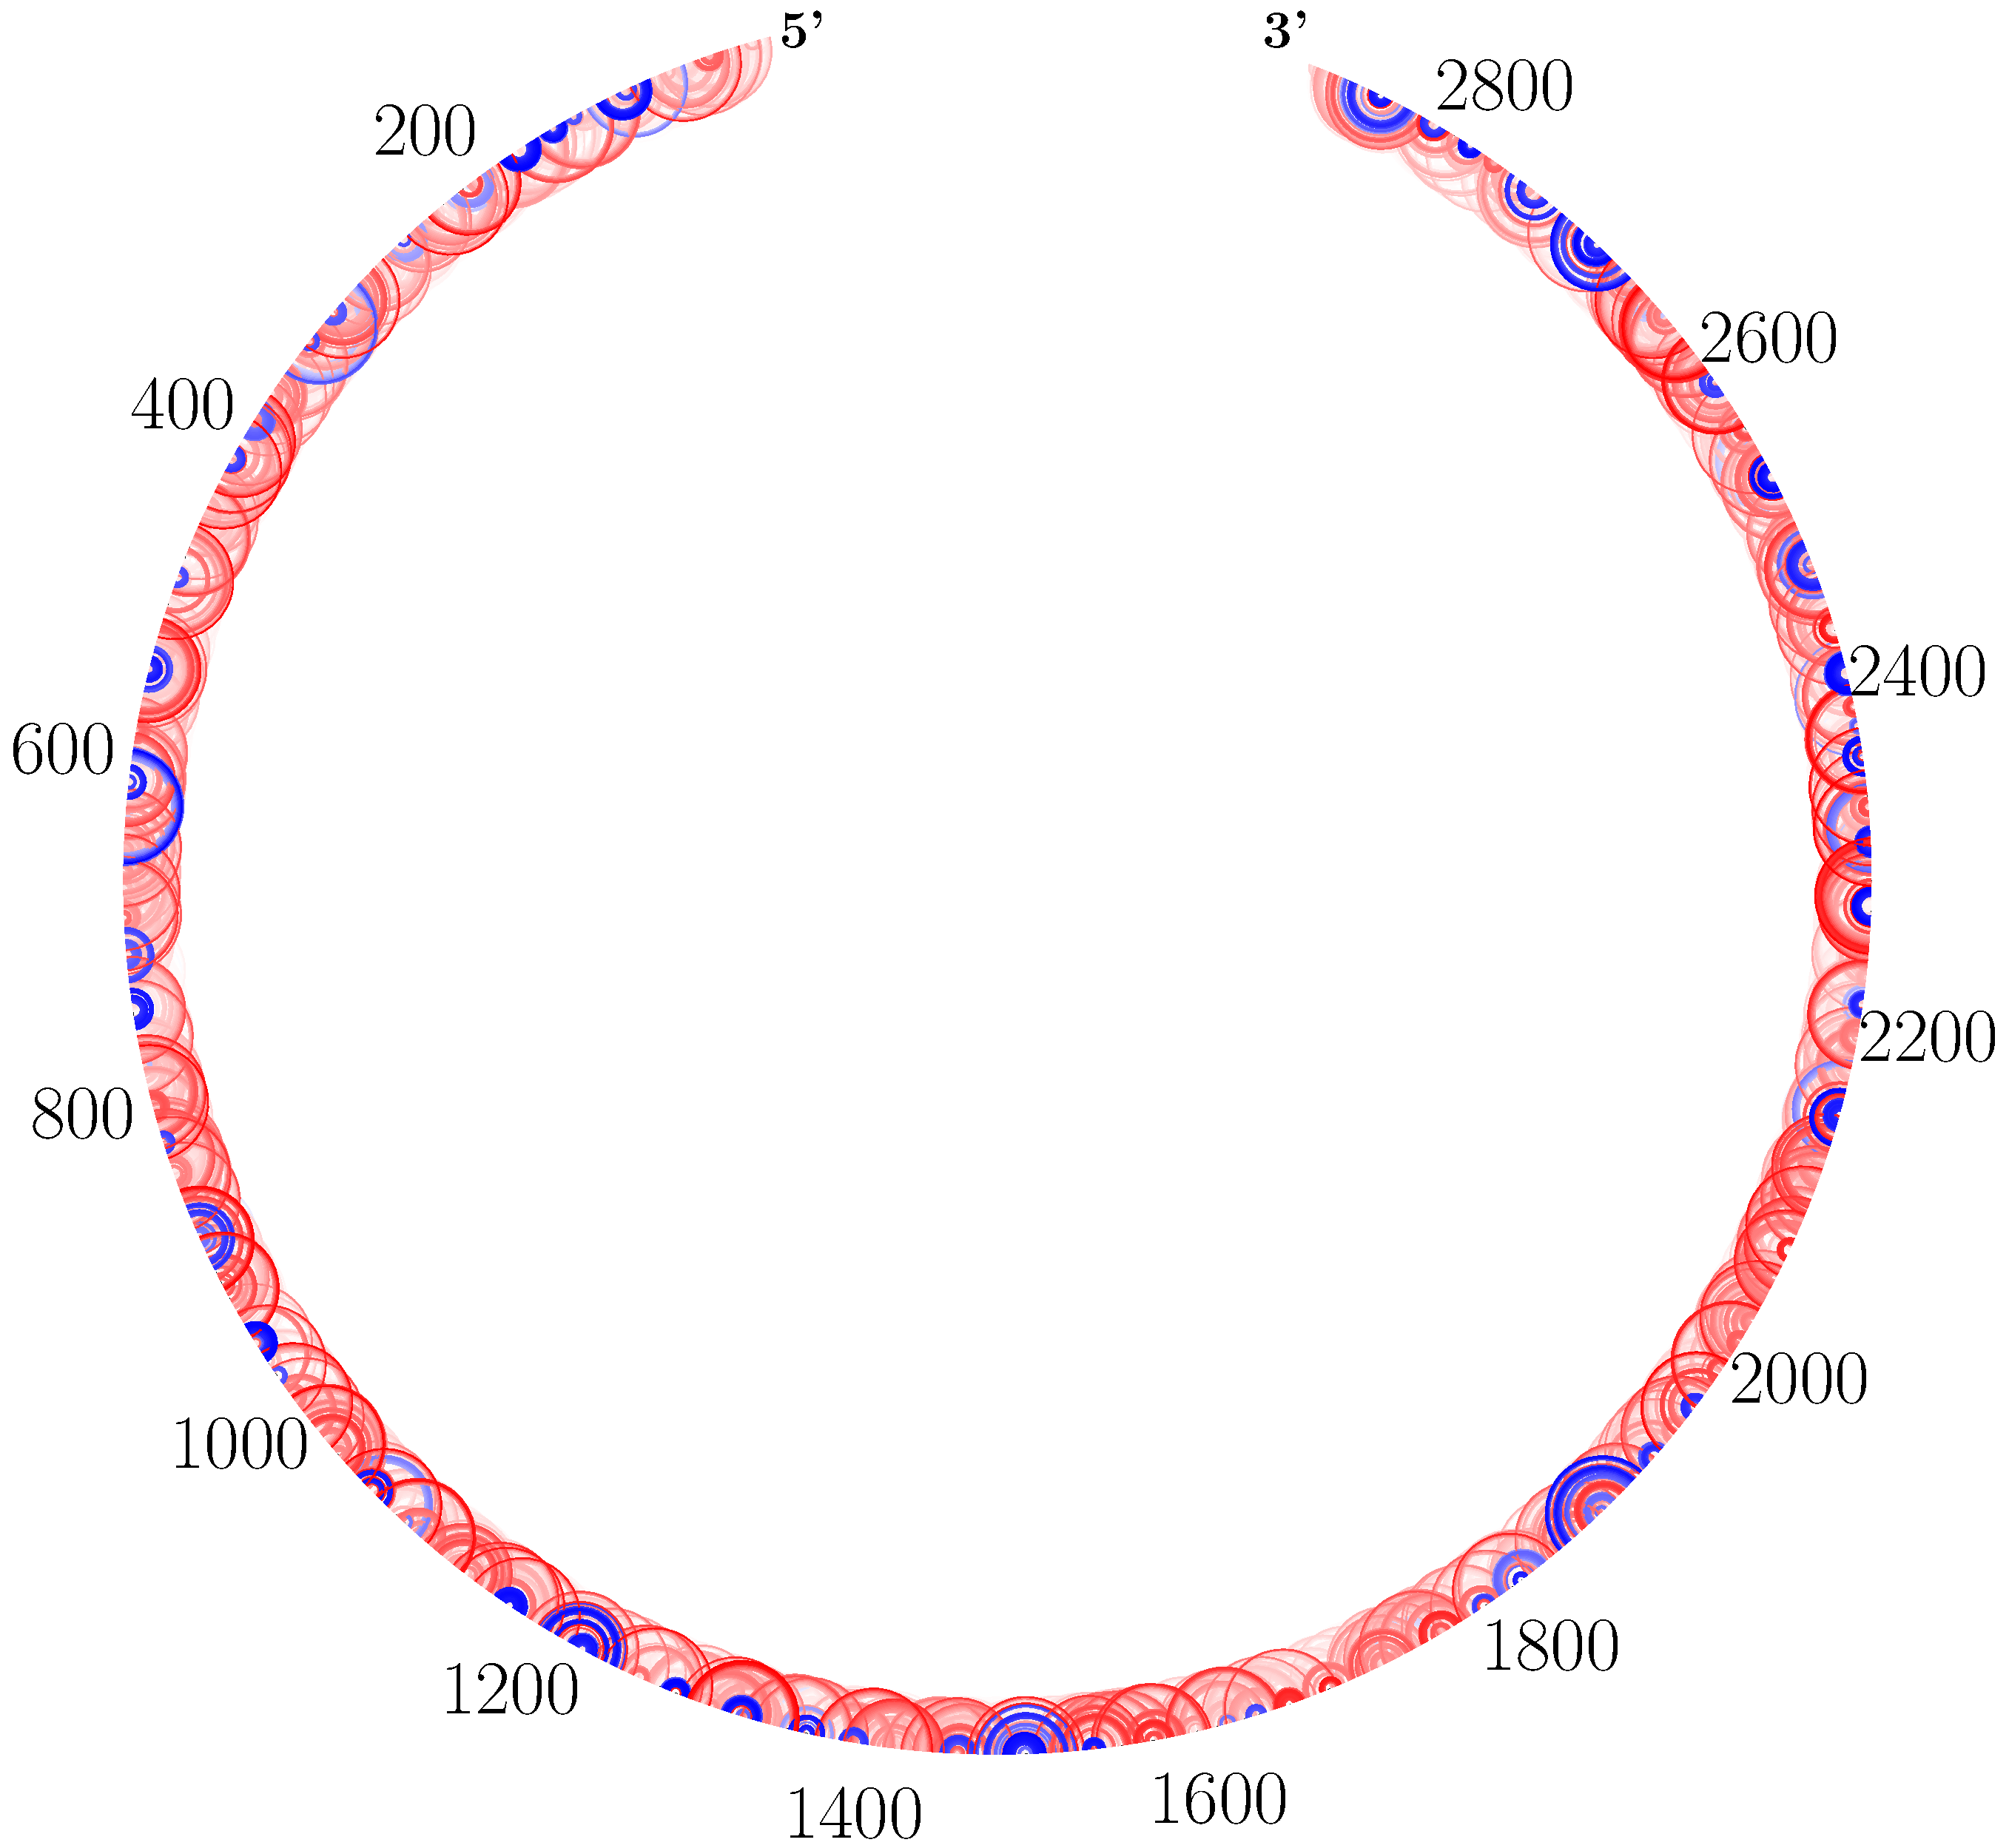
\includegraphics[width=0.25\textwidth]{figs/23s_vienna_plfold_example}} \\
% &&\hspace{-4.5cm}\panel{F}\\[-.3cm]
% &&\raisebox{0cm}{\hspace{0.2cm}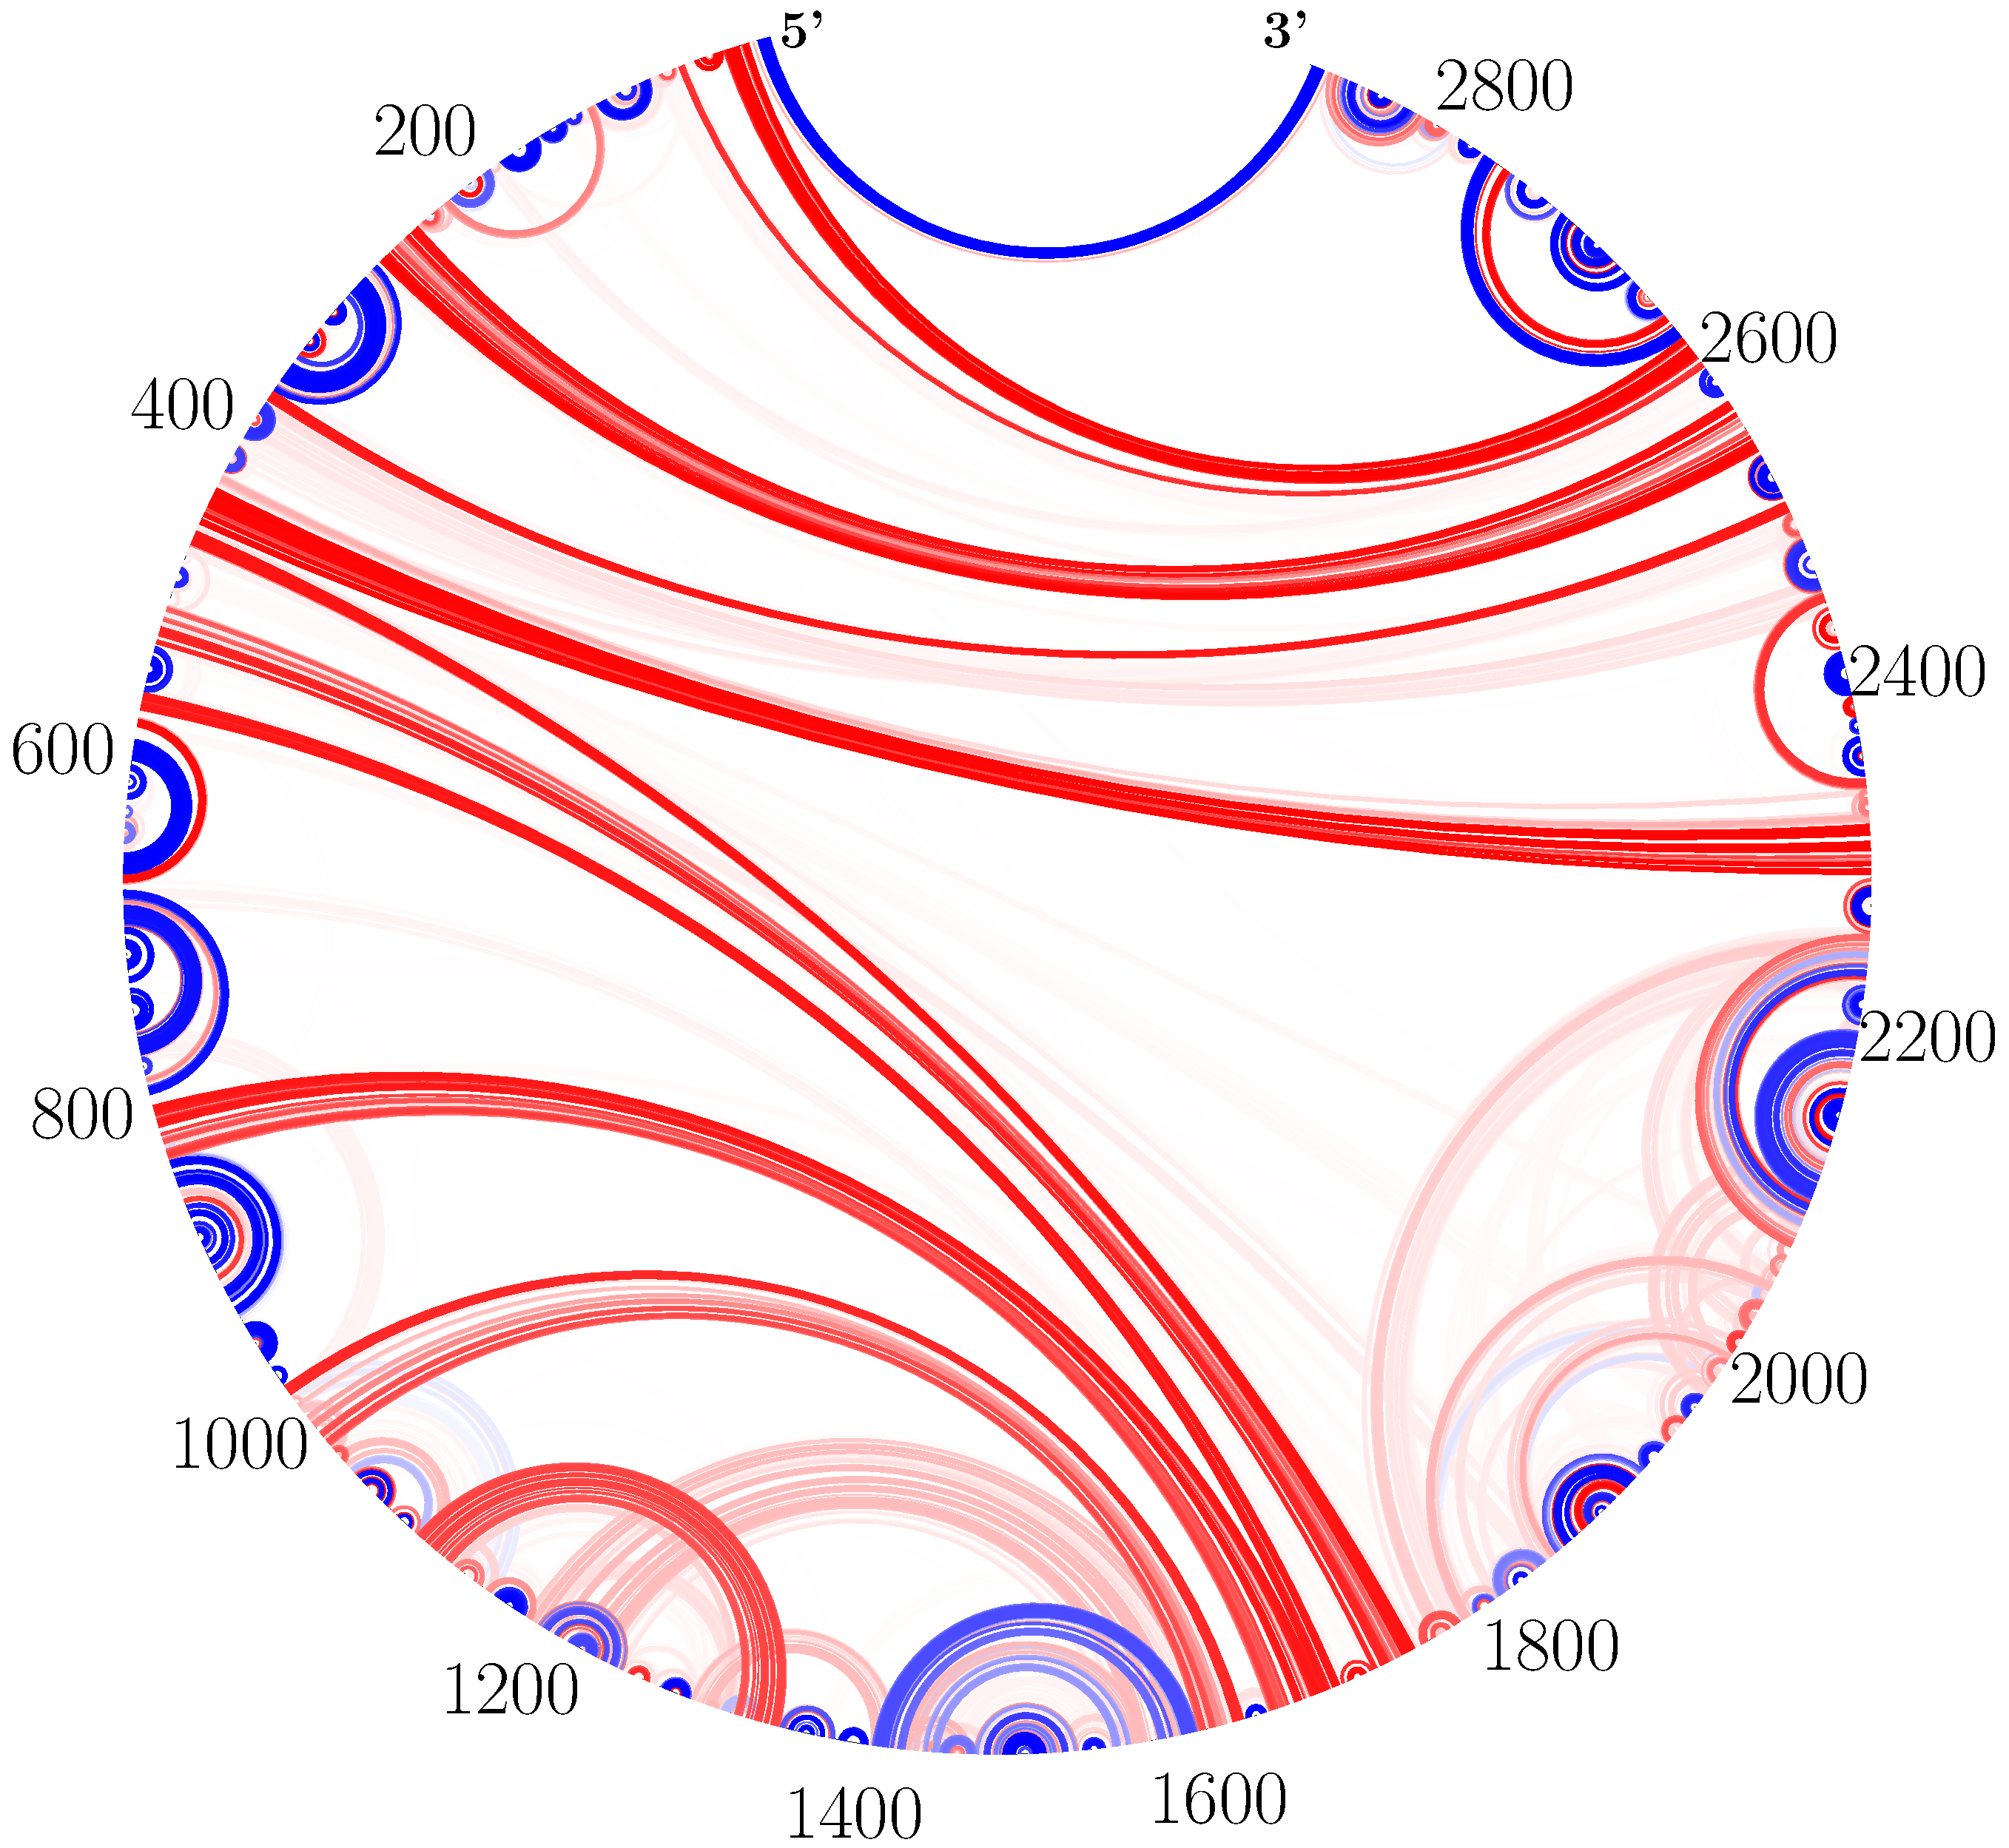
\includegraphics[width=0.25\textwidth]{figs/23s_vienna_example}} \\
% &&\hspace{-4.5cm}\panel{G}\\[-.3cm]
% &&\raisebox{0cm}{\hspace{0.2cm}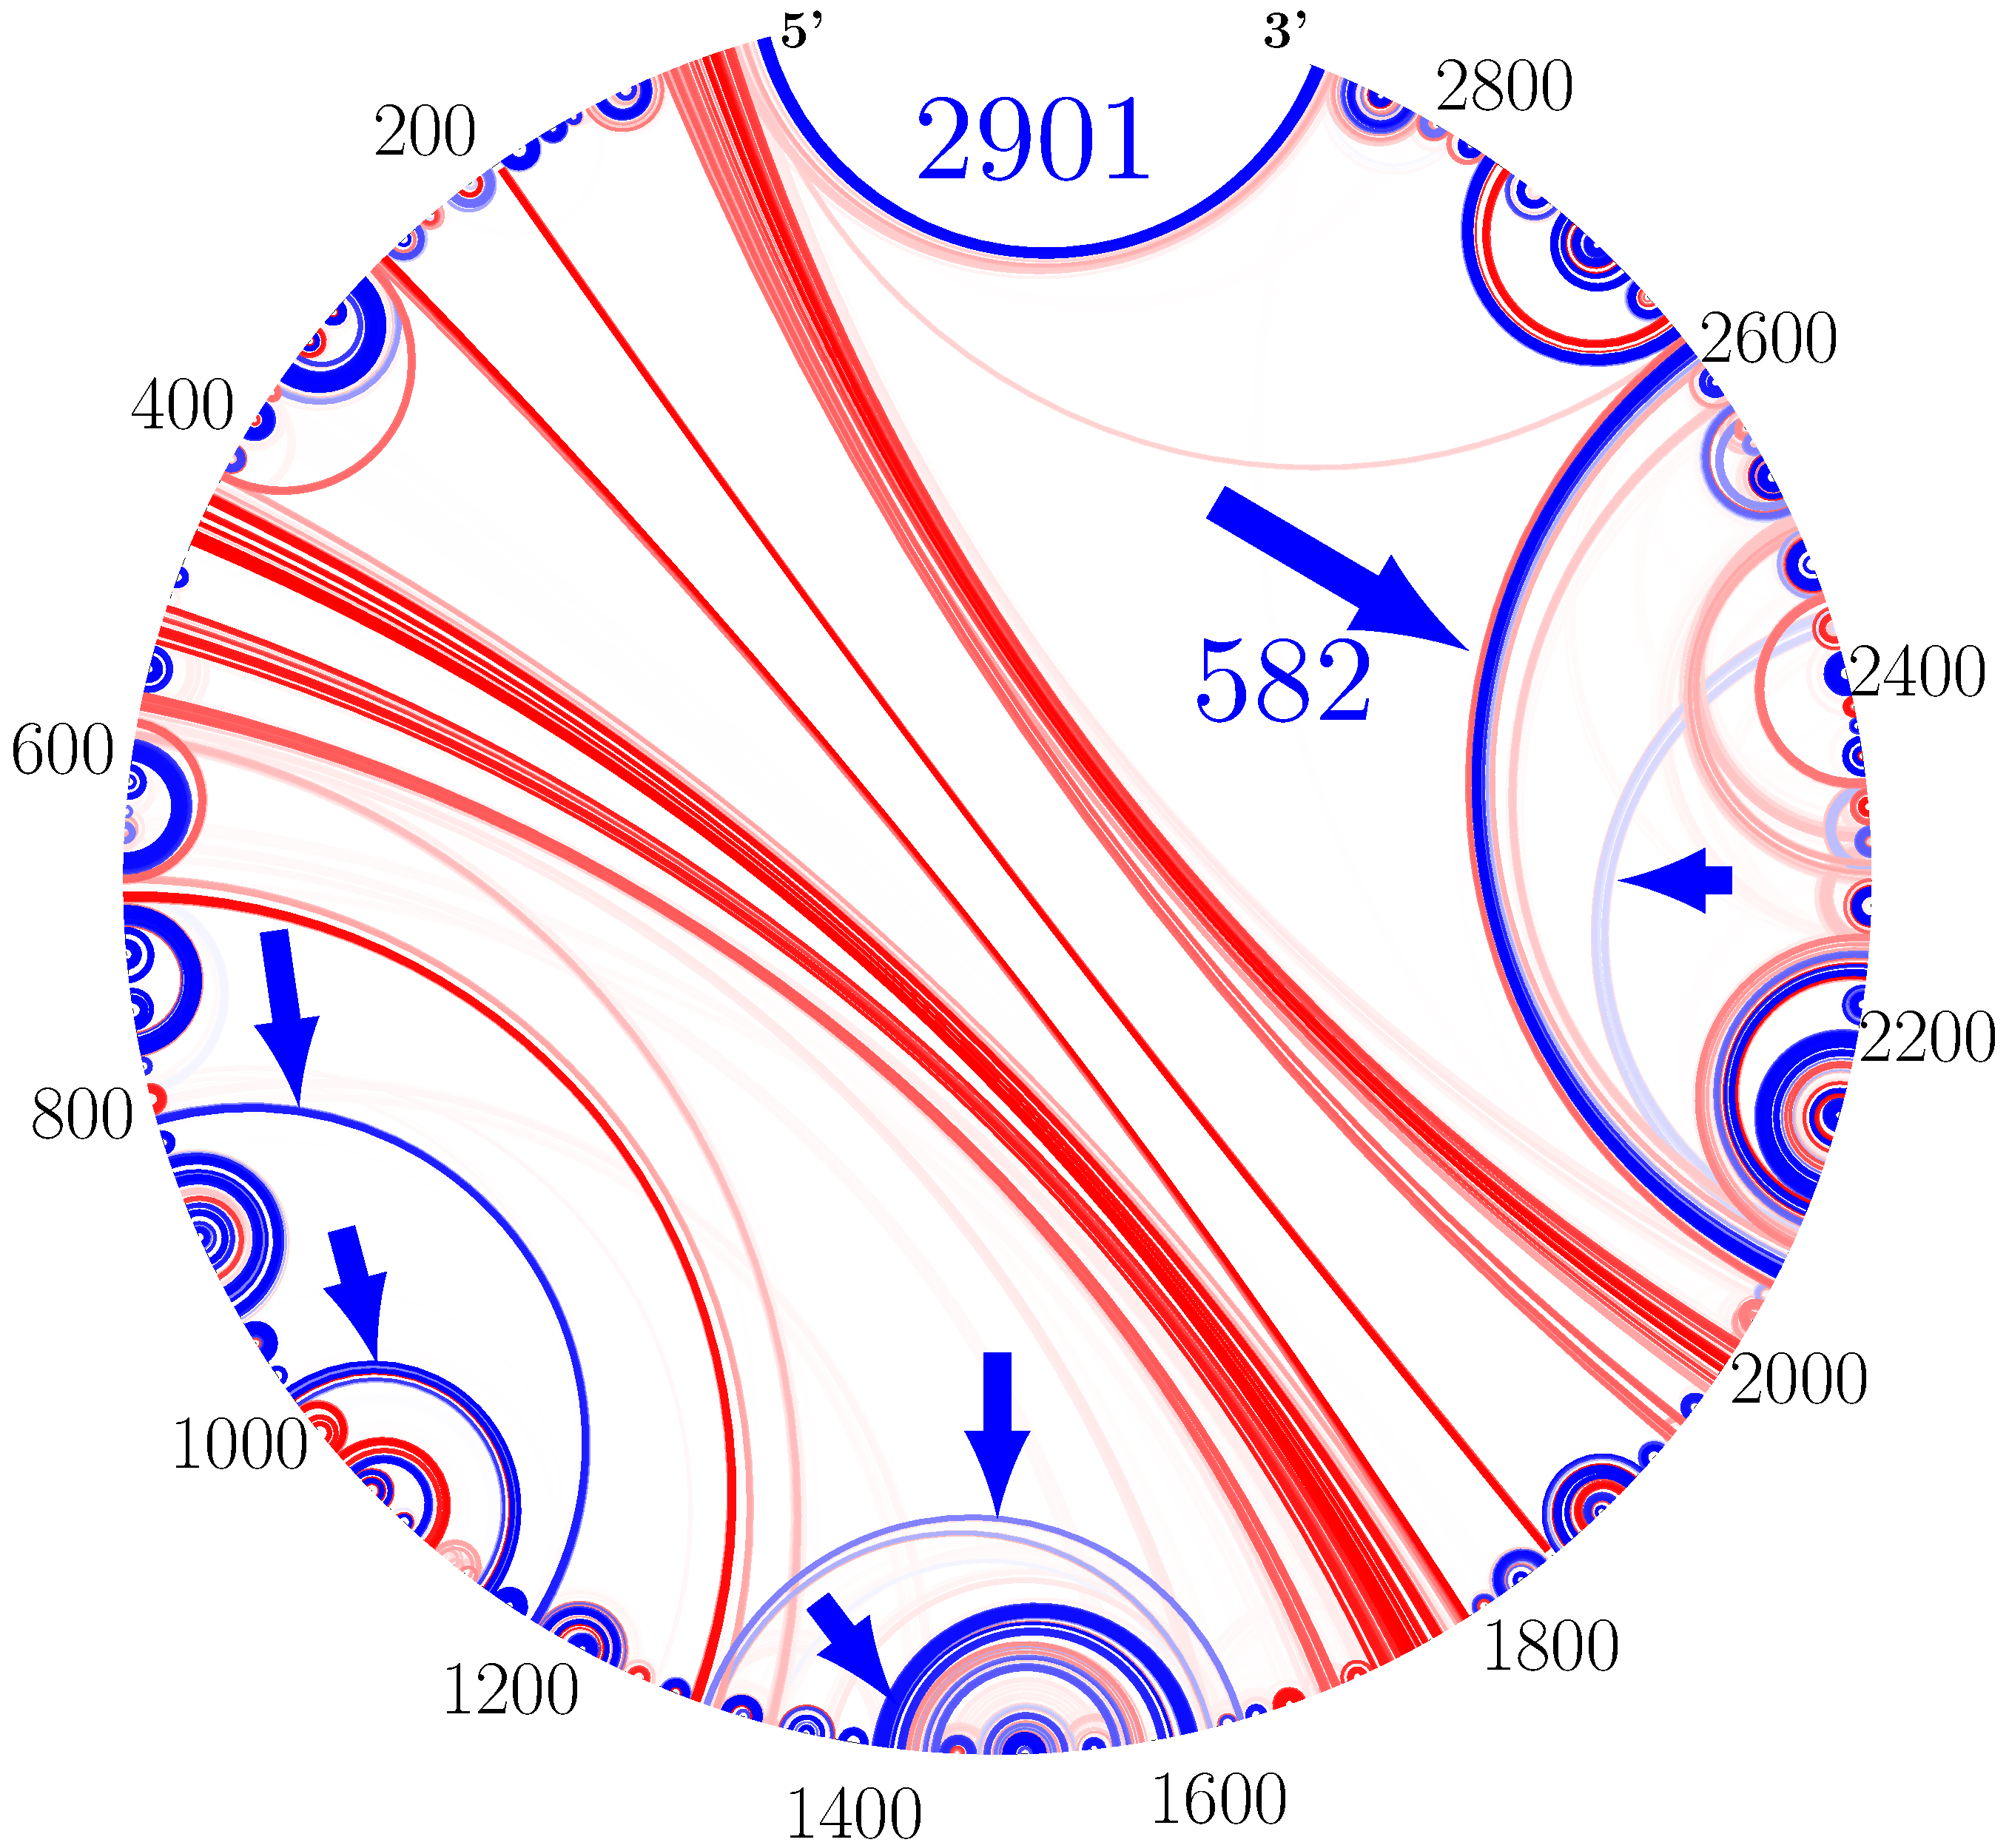
\includegraphics[width=0.25\textwidth]{figs/23s_example}} \\[-2.3cm]
% % } & \\[-.4cm]
% \hspace{-.2cm}\raisebox{1cm}{\panel{C}} & \\[-2.2cm]
% \hspace{-7cm}\panel{E} &\\[-.5cm]
% \multicolumn{2}{l}{% \hspace{-0.3cm}

\resizebox{0.5\textwidth}{!}
{
  \begin{tabular}{c}
%	\toprule
         % &     \multicolumn{2}{c}{total} & \multicolumn{2}{c}{correct} \\
			 % \midrule
\hspace{6.5cm}{\color{blue} $p_\linear \!-\! p_\vienna \!>\! 0.2$} \\[.3cm]
\hspace{6.4cm}{\color{darkgreen} $|p_\linear \!-\! p_\vienna| \!\leq \!0.2$} \\[.3cm]
\hspace{6.3cm}{\color{red} $p_\linear \!-\! p_\vienna \!<\! -0.2$}  \\[-2.4cm]
%	                 \bottomrule
  \end{tabular}
 }

% \resizebox{0.45\textwidth}{!}
% \panel{C}}
\vspace{.5cm}
{
  \hspace{-4.5cm}\begin{tabular}{r@{\; }r@{\quad}r@{\; }r}
%	\toprule
% \panel{C}} & &&\\
          \multicolumn{2}{c}{total} & \multicolumn{2}{c}{correct} \\
			 \midrule
55 \bluetri & 40 \bluecir  & 23 \bluetri & 37 \bluecir \\
  126,645 \greentri & 420 \greencir & 111 \greentri & 180 \greencir\\
 56 \redtri & 44 \redcir & 0 \redtri & 19 \redcir \\[1.9cm]
%	                 \bottomrule
  \end{tabular}
  }

% }
% &\\[-2cm]
% &\raisebox{5cm}{\hspace{-0.2cm}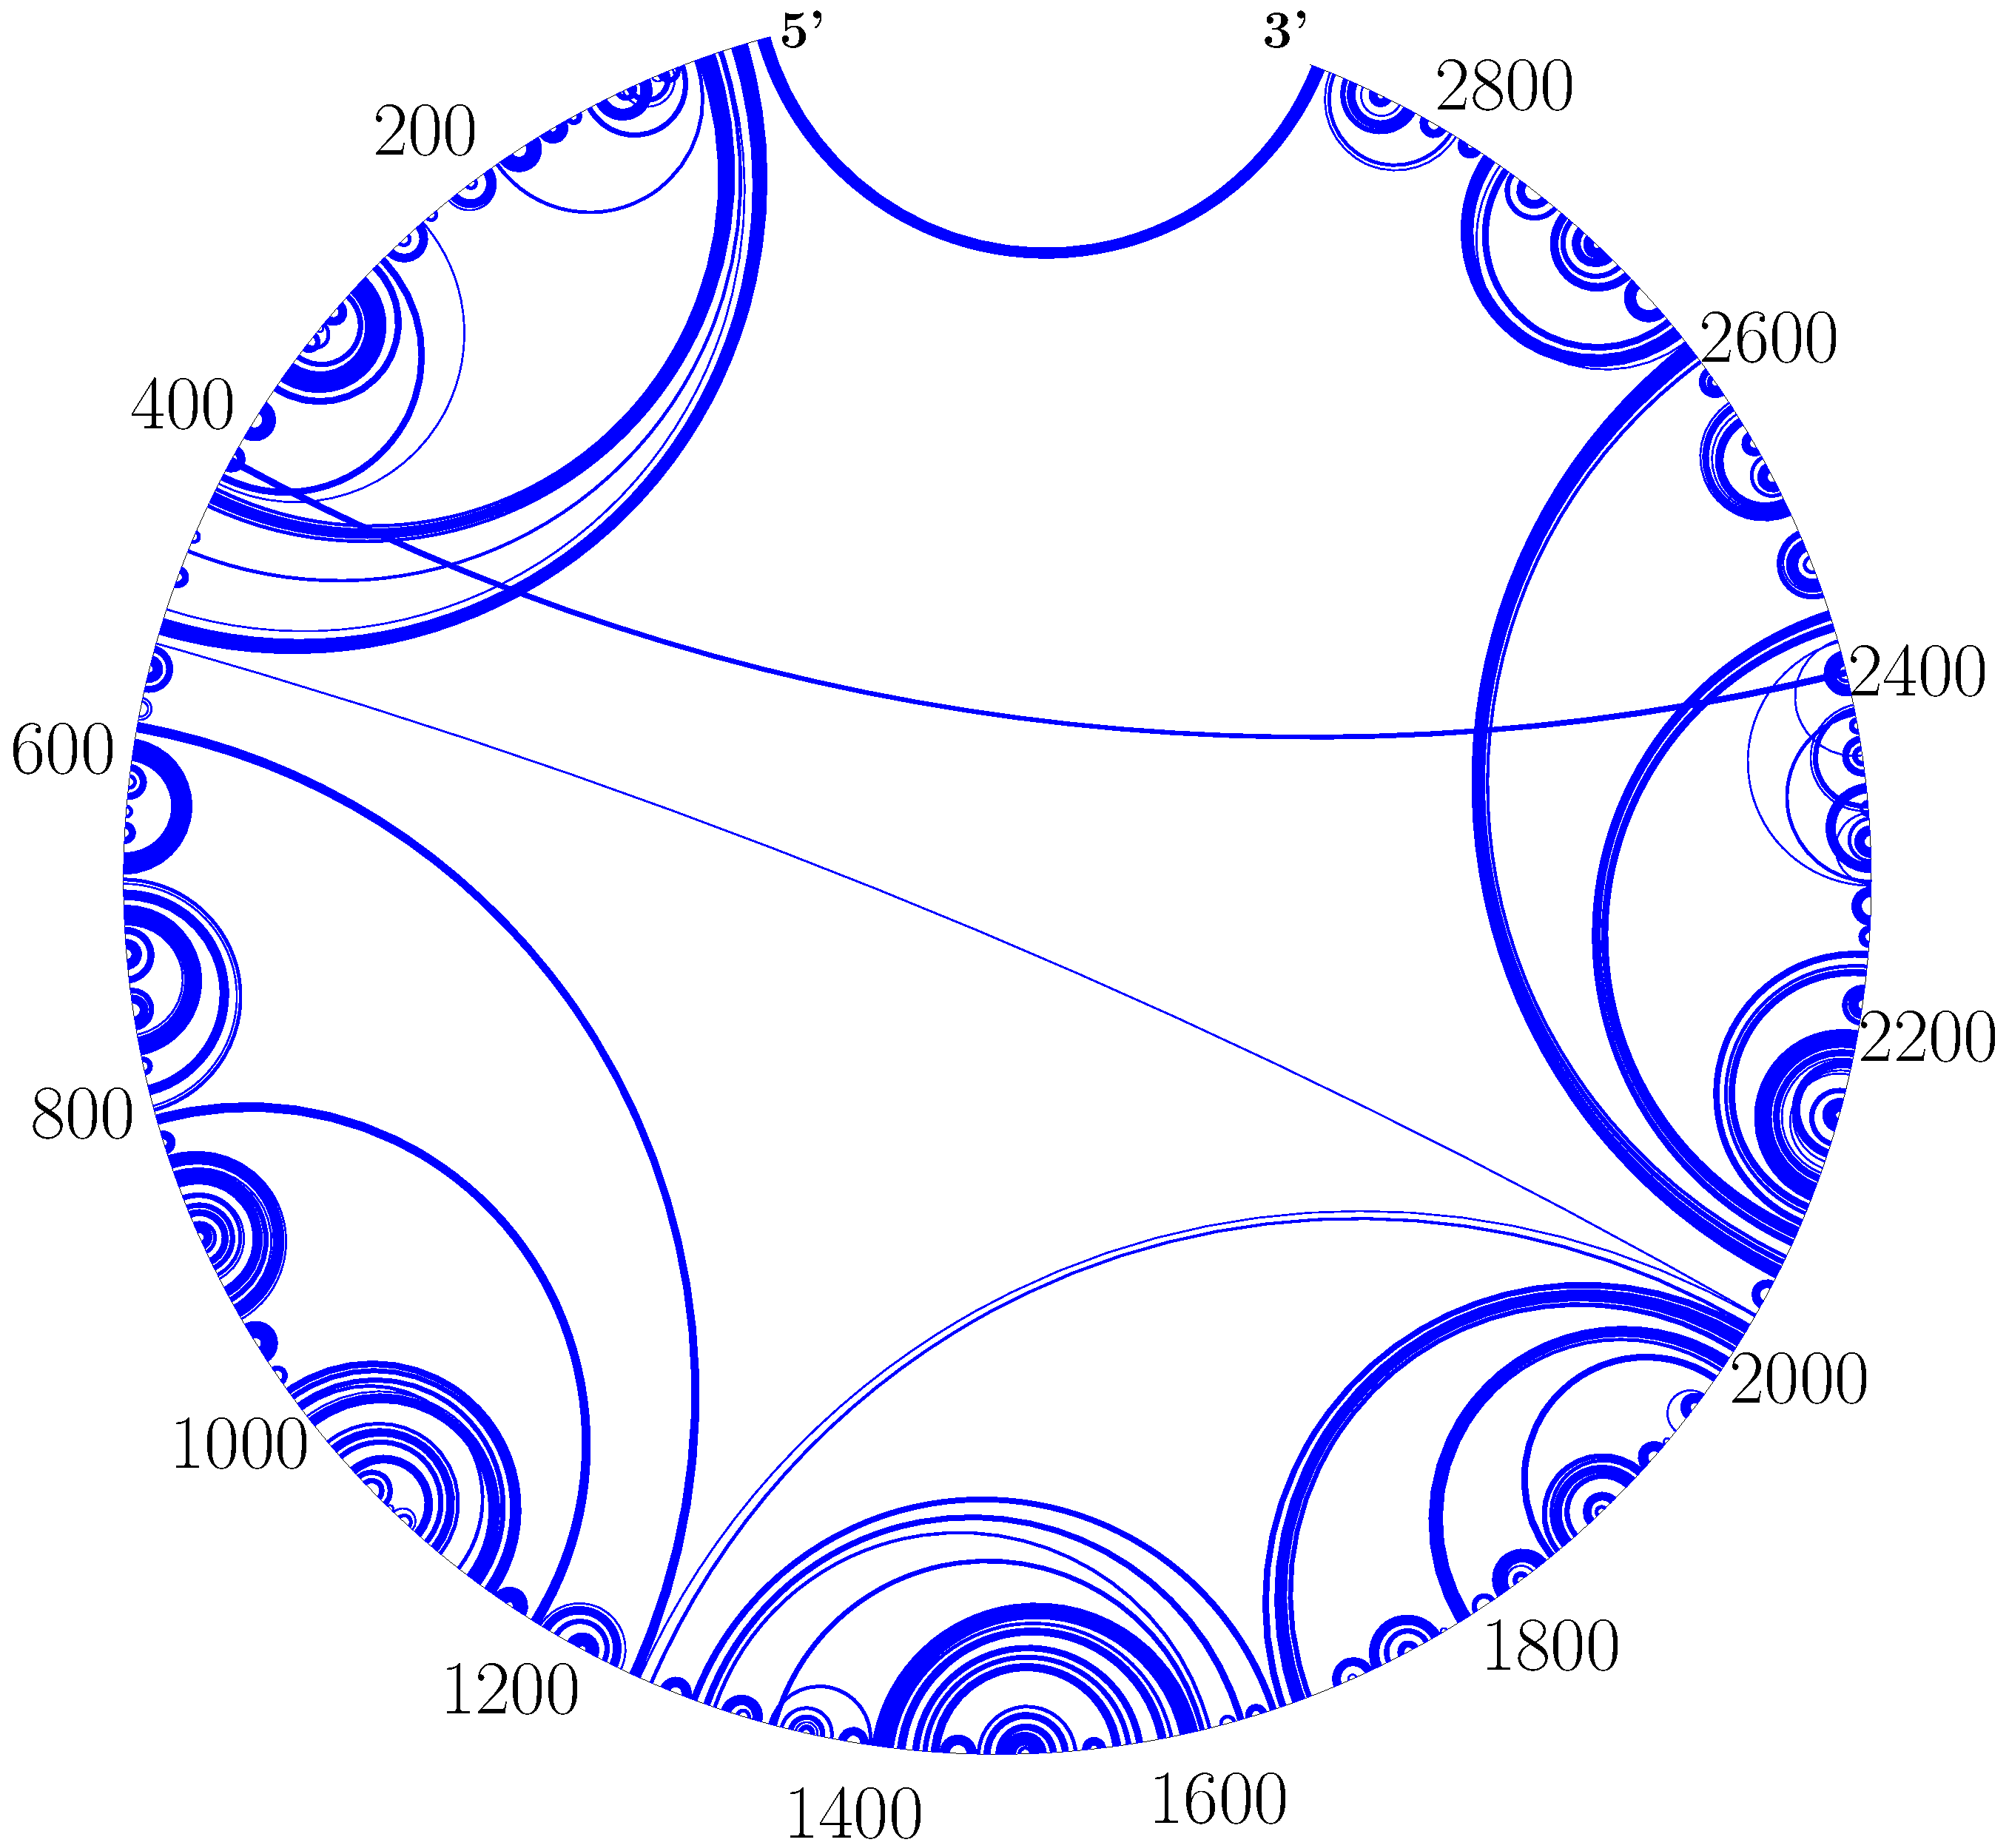
\includegraphics[width=0.25\textwidth]{figs/23s_gold}} \\
% \end{tabular}\\

% \begin{tabular}{cccc}
% \hspace{-4.4cm} \panel{F} & \hspace{-4.6cm}\panel{G} & \hspace{-4.6cm}\panel{H} & \hspace{-4.6cm}\panel{I}\\[-0.2cm]
% \hspace{-0.2cm}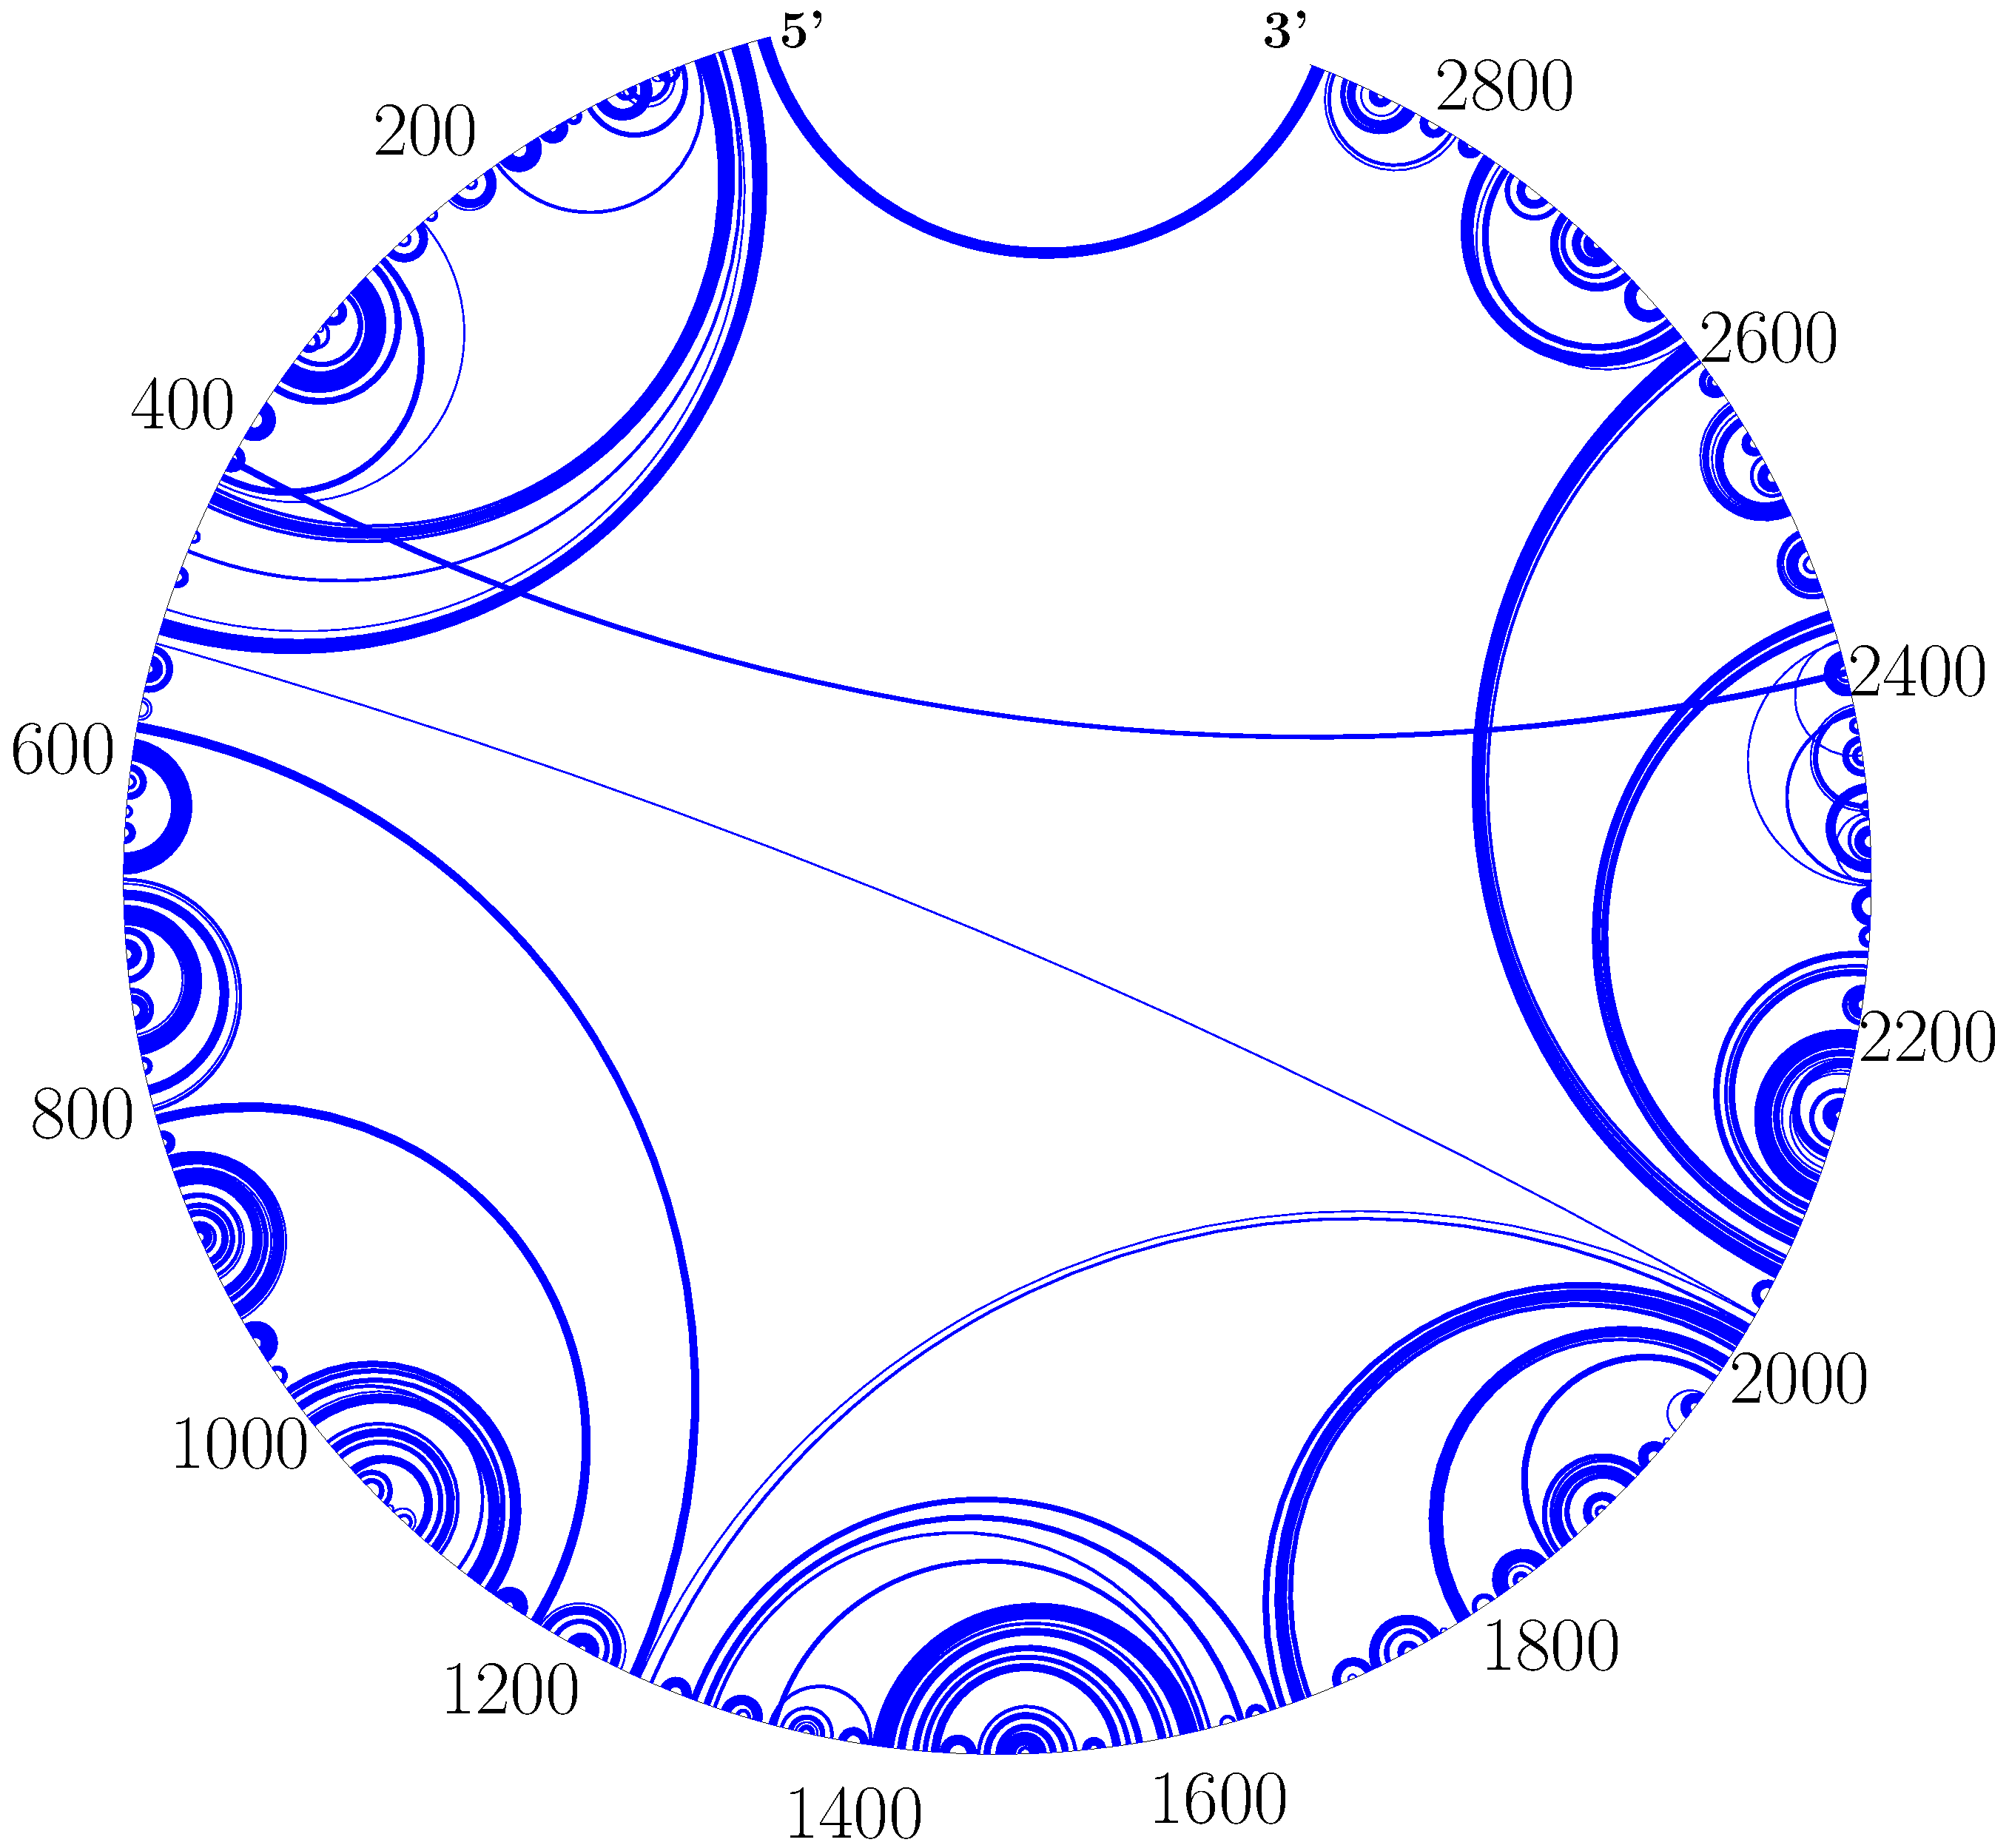
\includegraphics[width=0.25\textwidth]{figs/23s_gold} &
% \hspace{-0.35cm}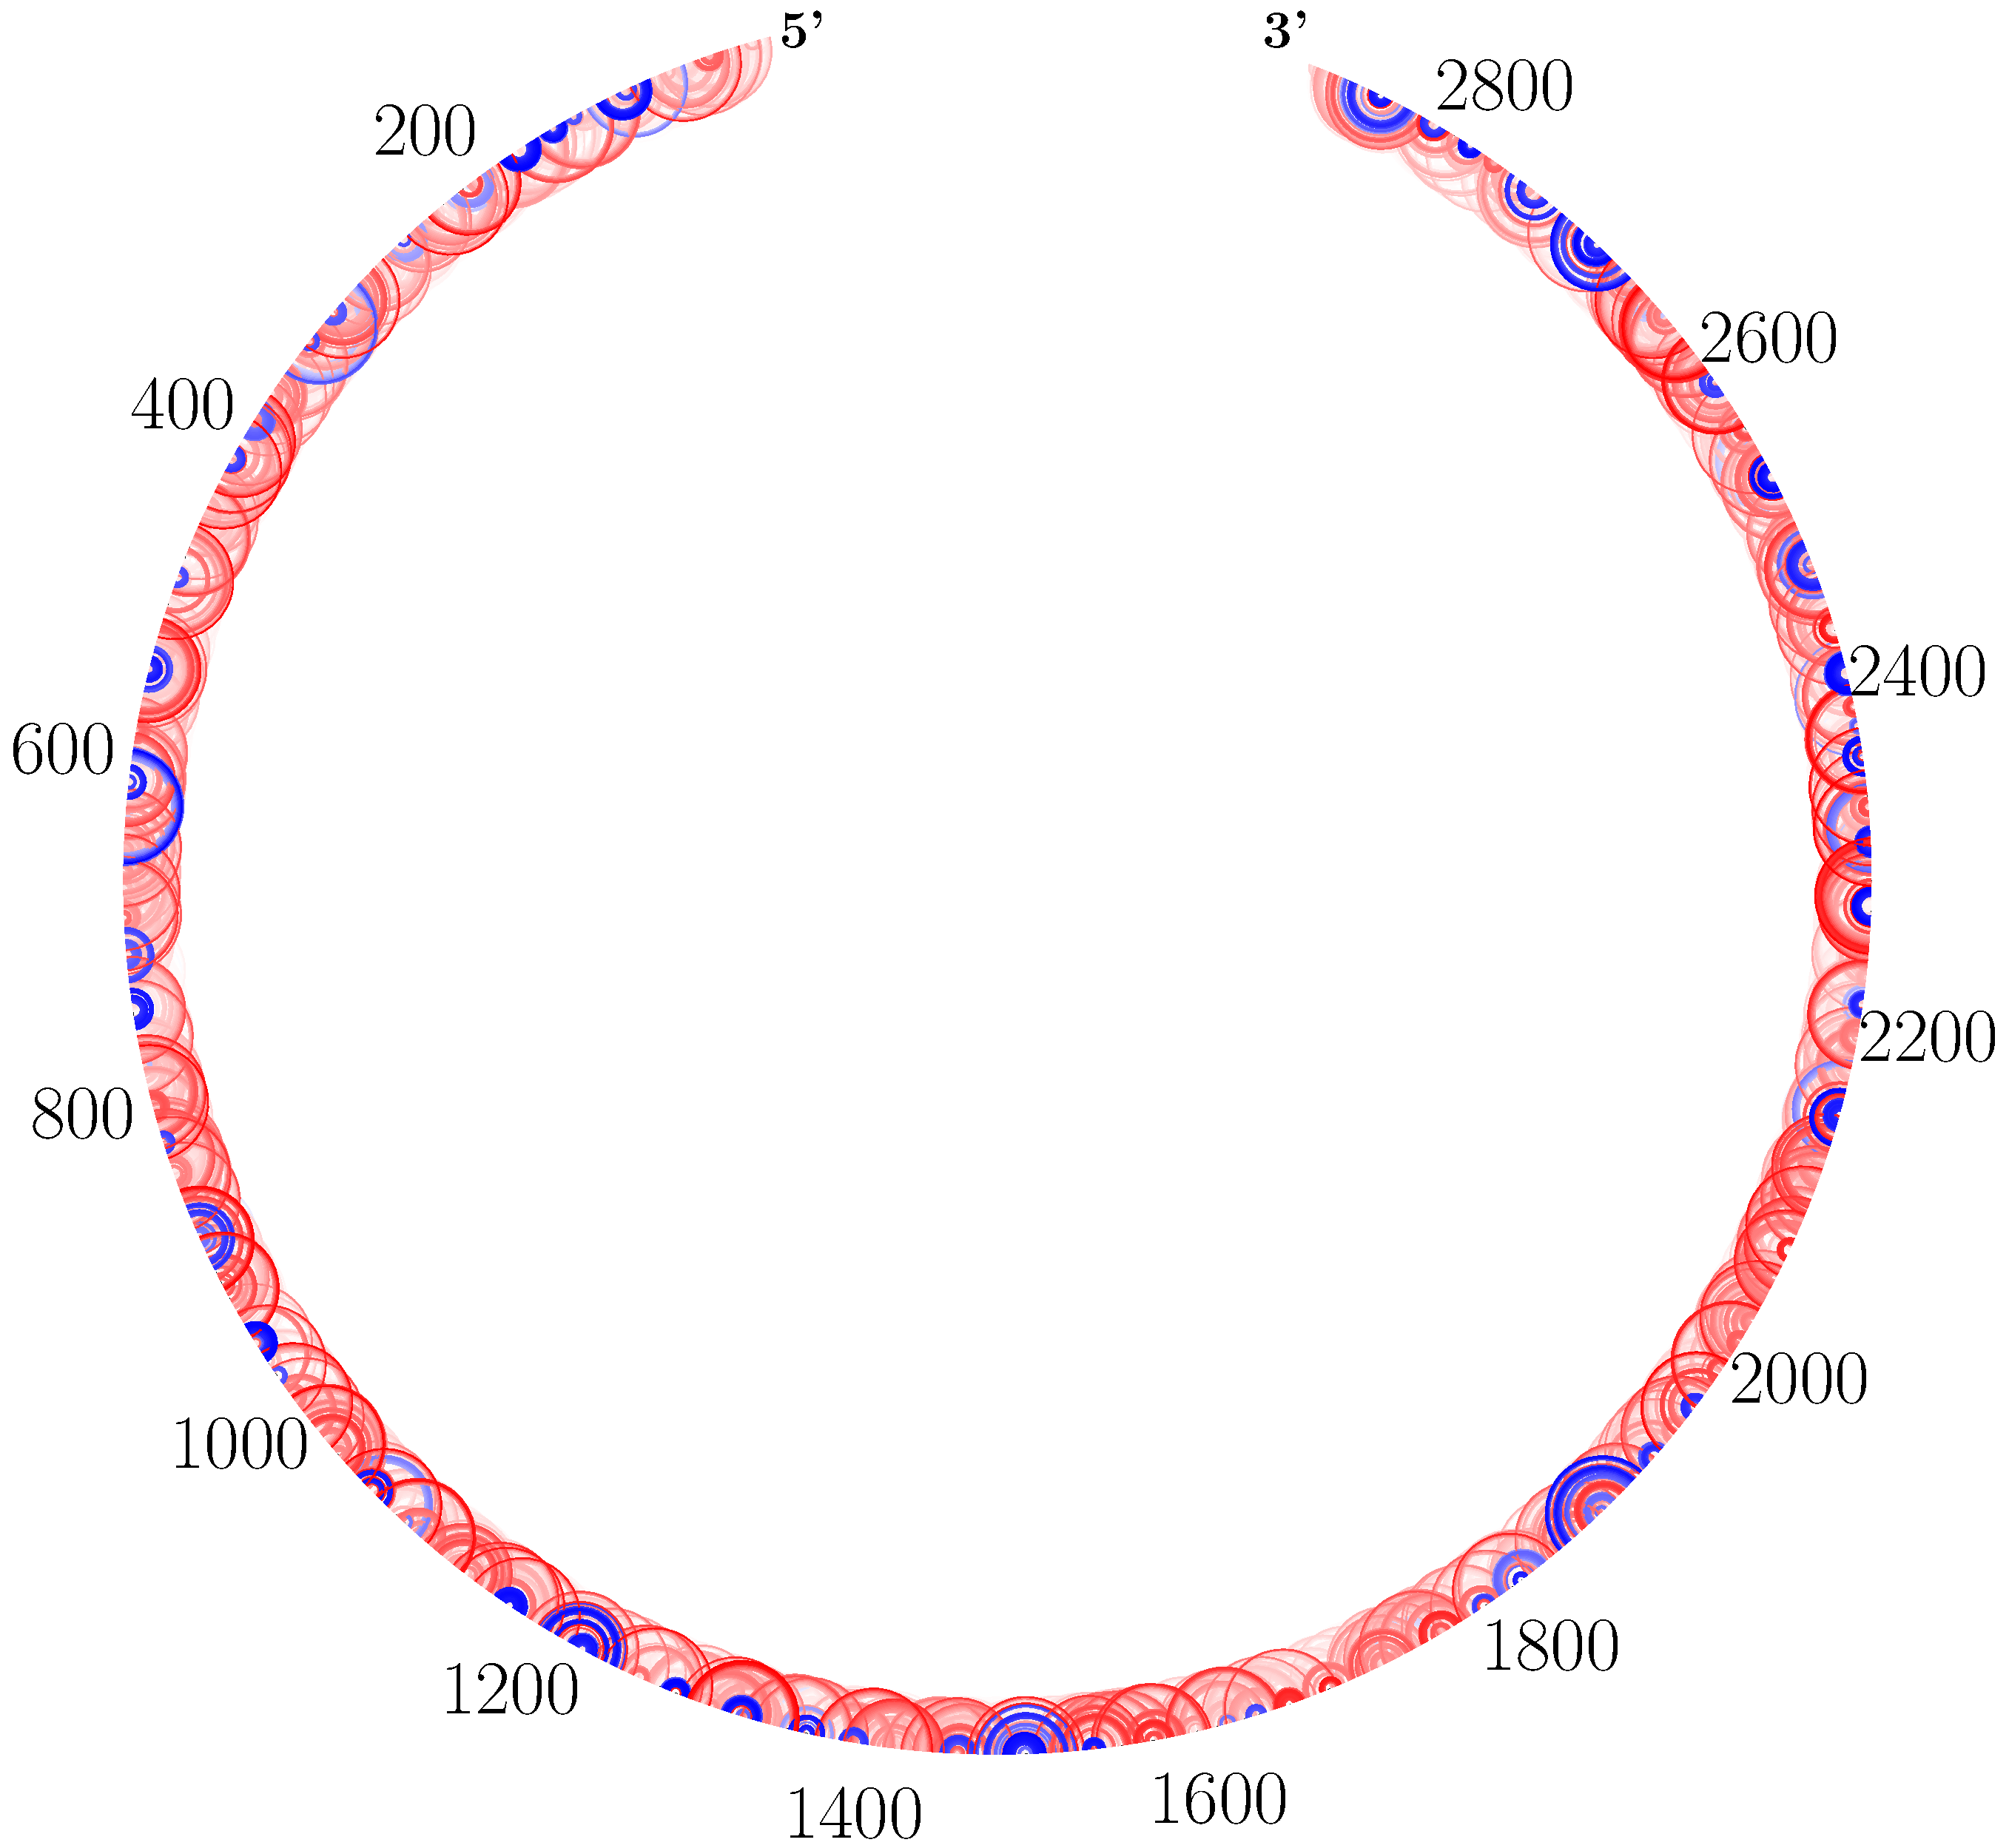
\includegraphics[width=0.25\textwidth]{figs/23s_vienna_plfold_example.pdf} &
% \hspace{-0.35cm}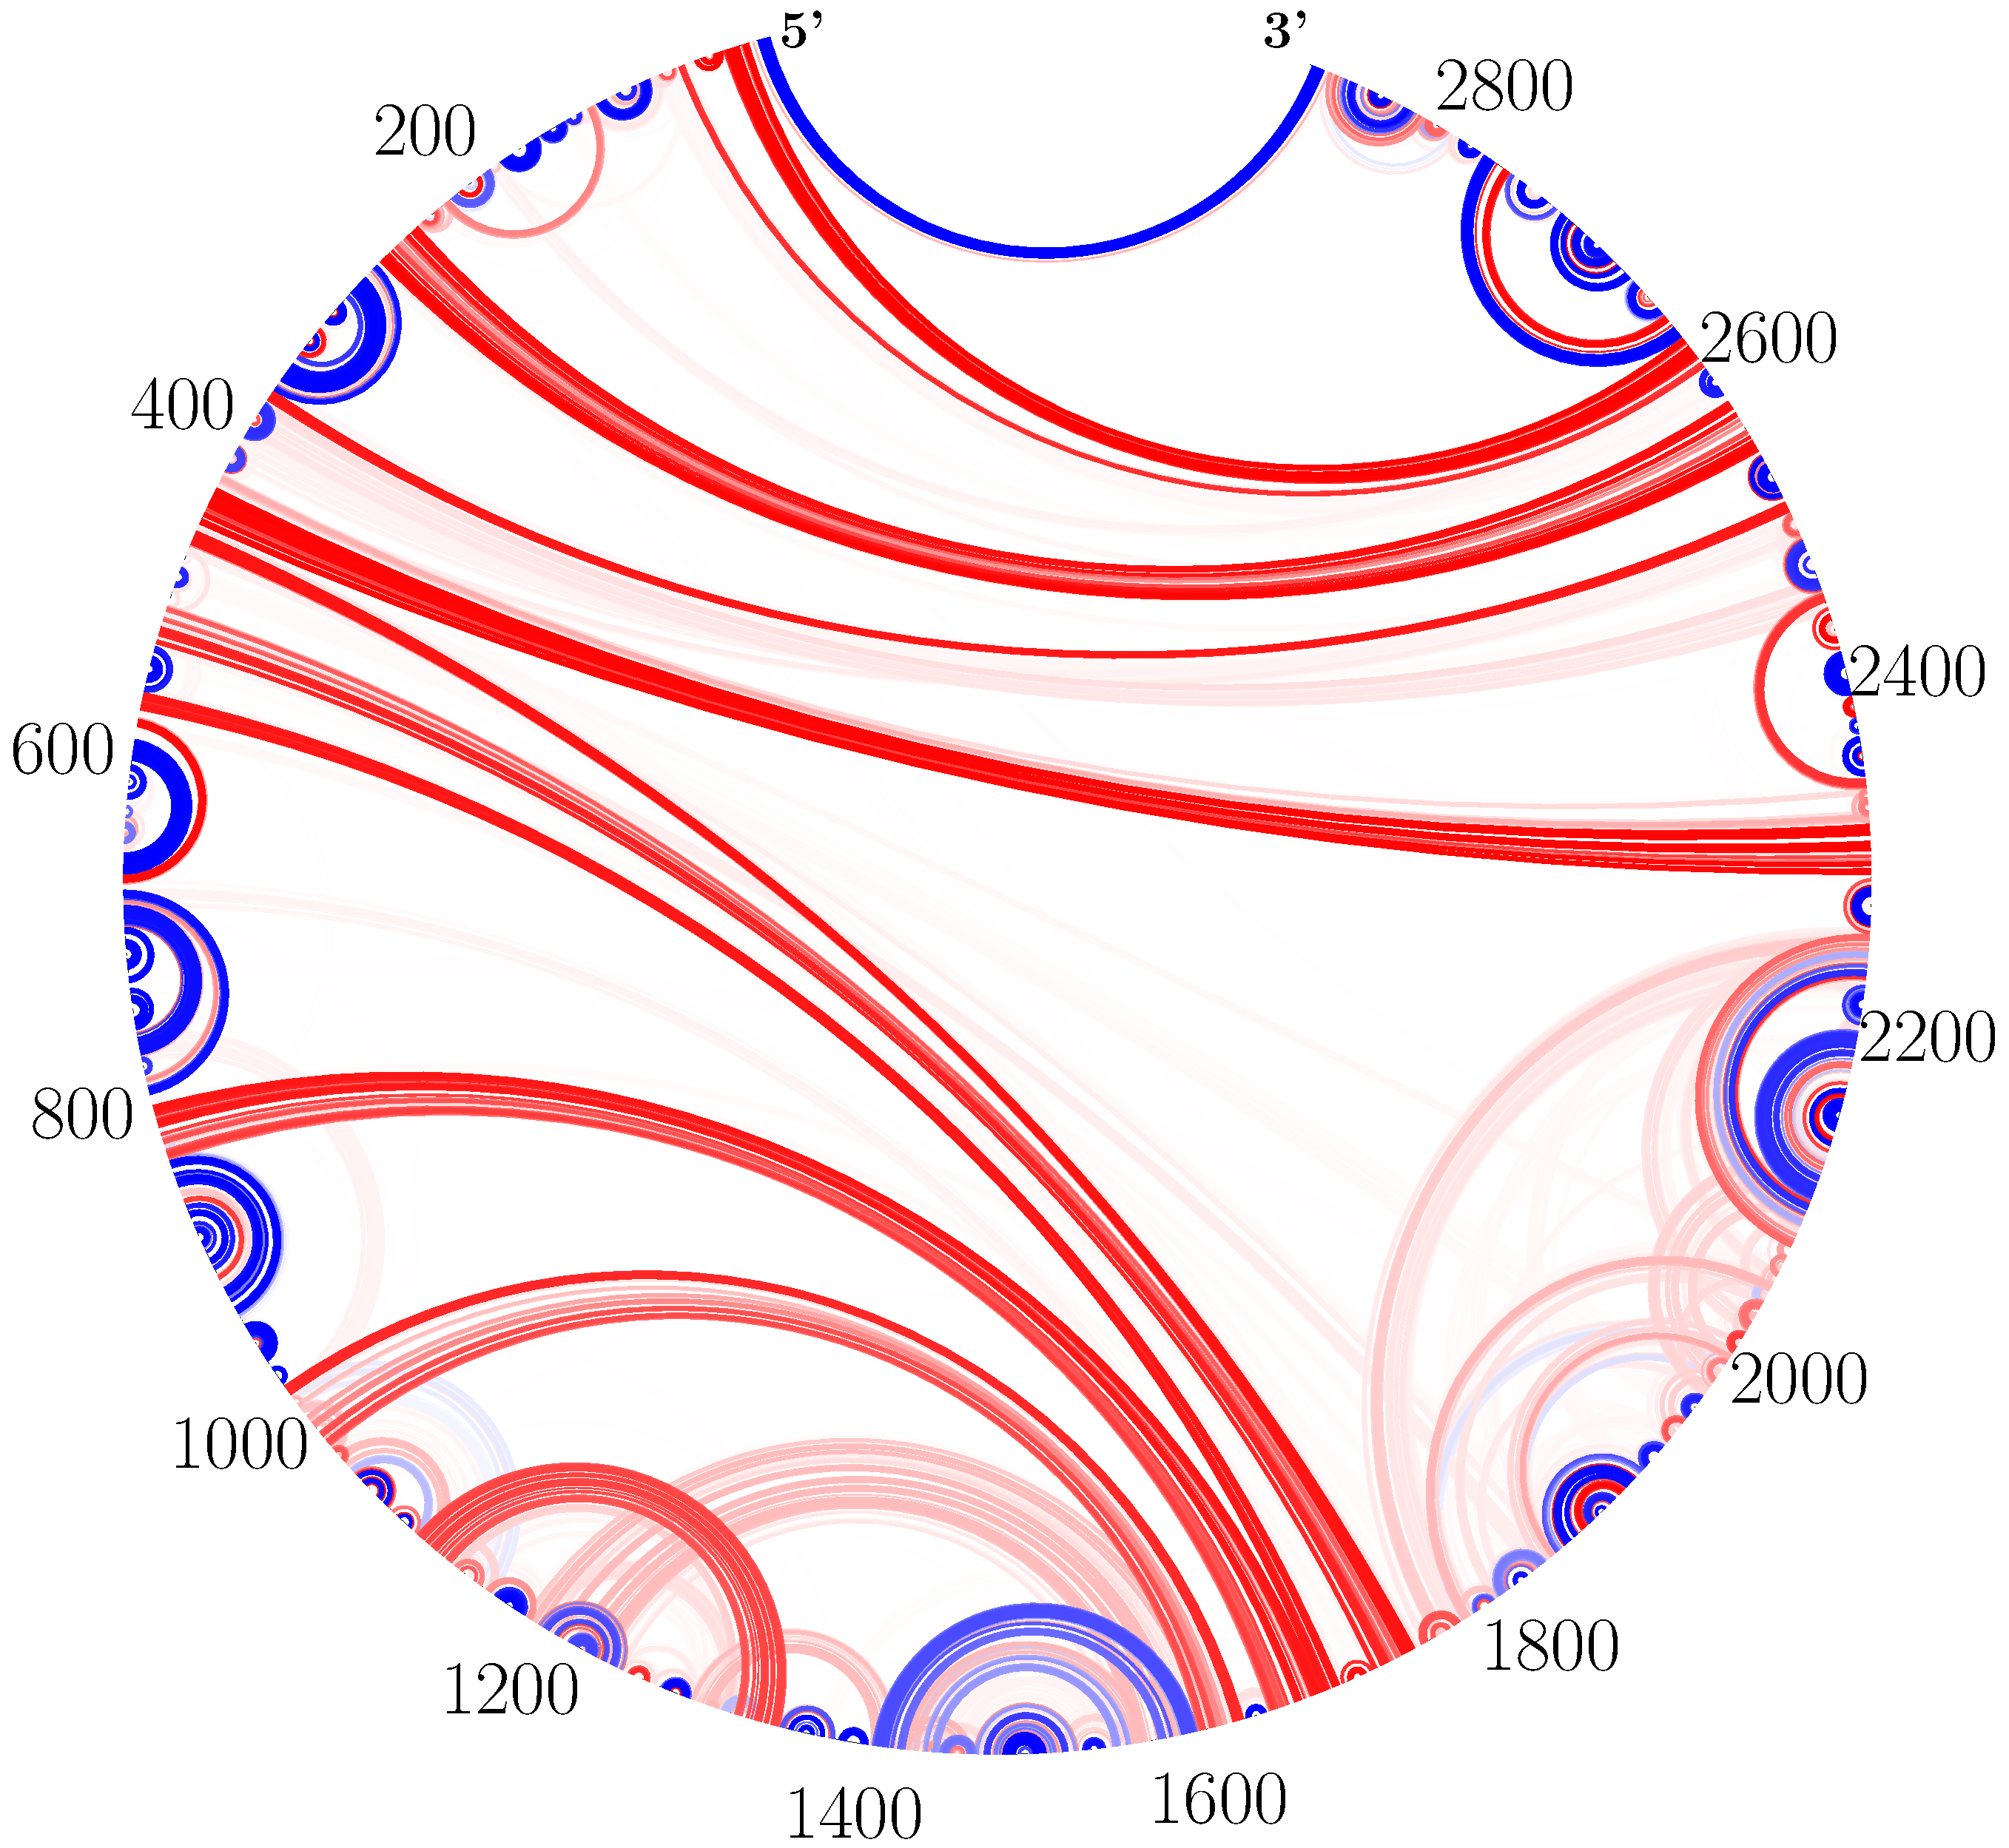
\includegraphics[width=0.25\textwidth]{figs/23s_vienna_example} &
% \hspace{-0.35cm}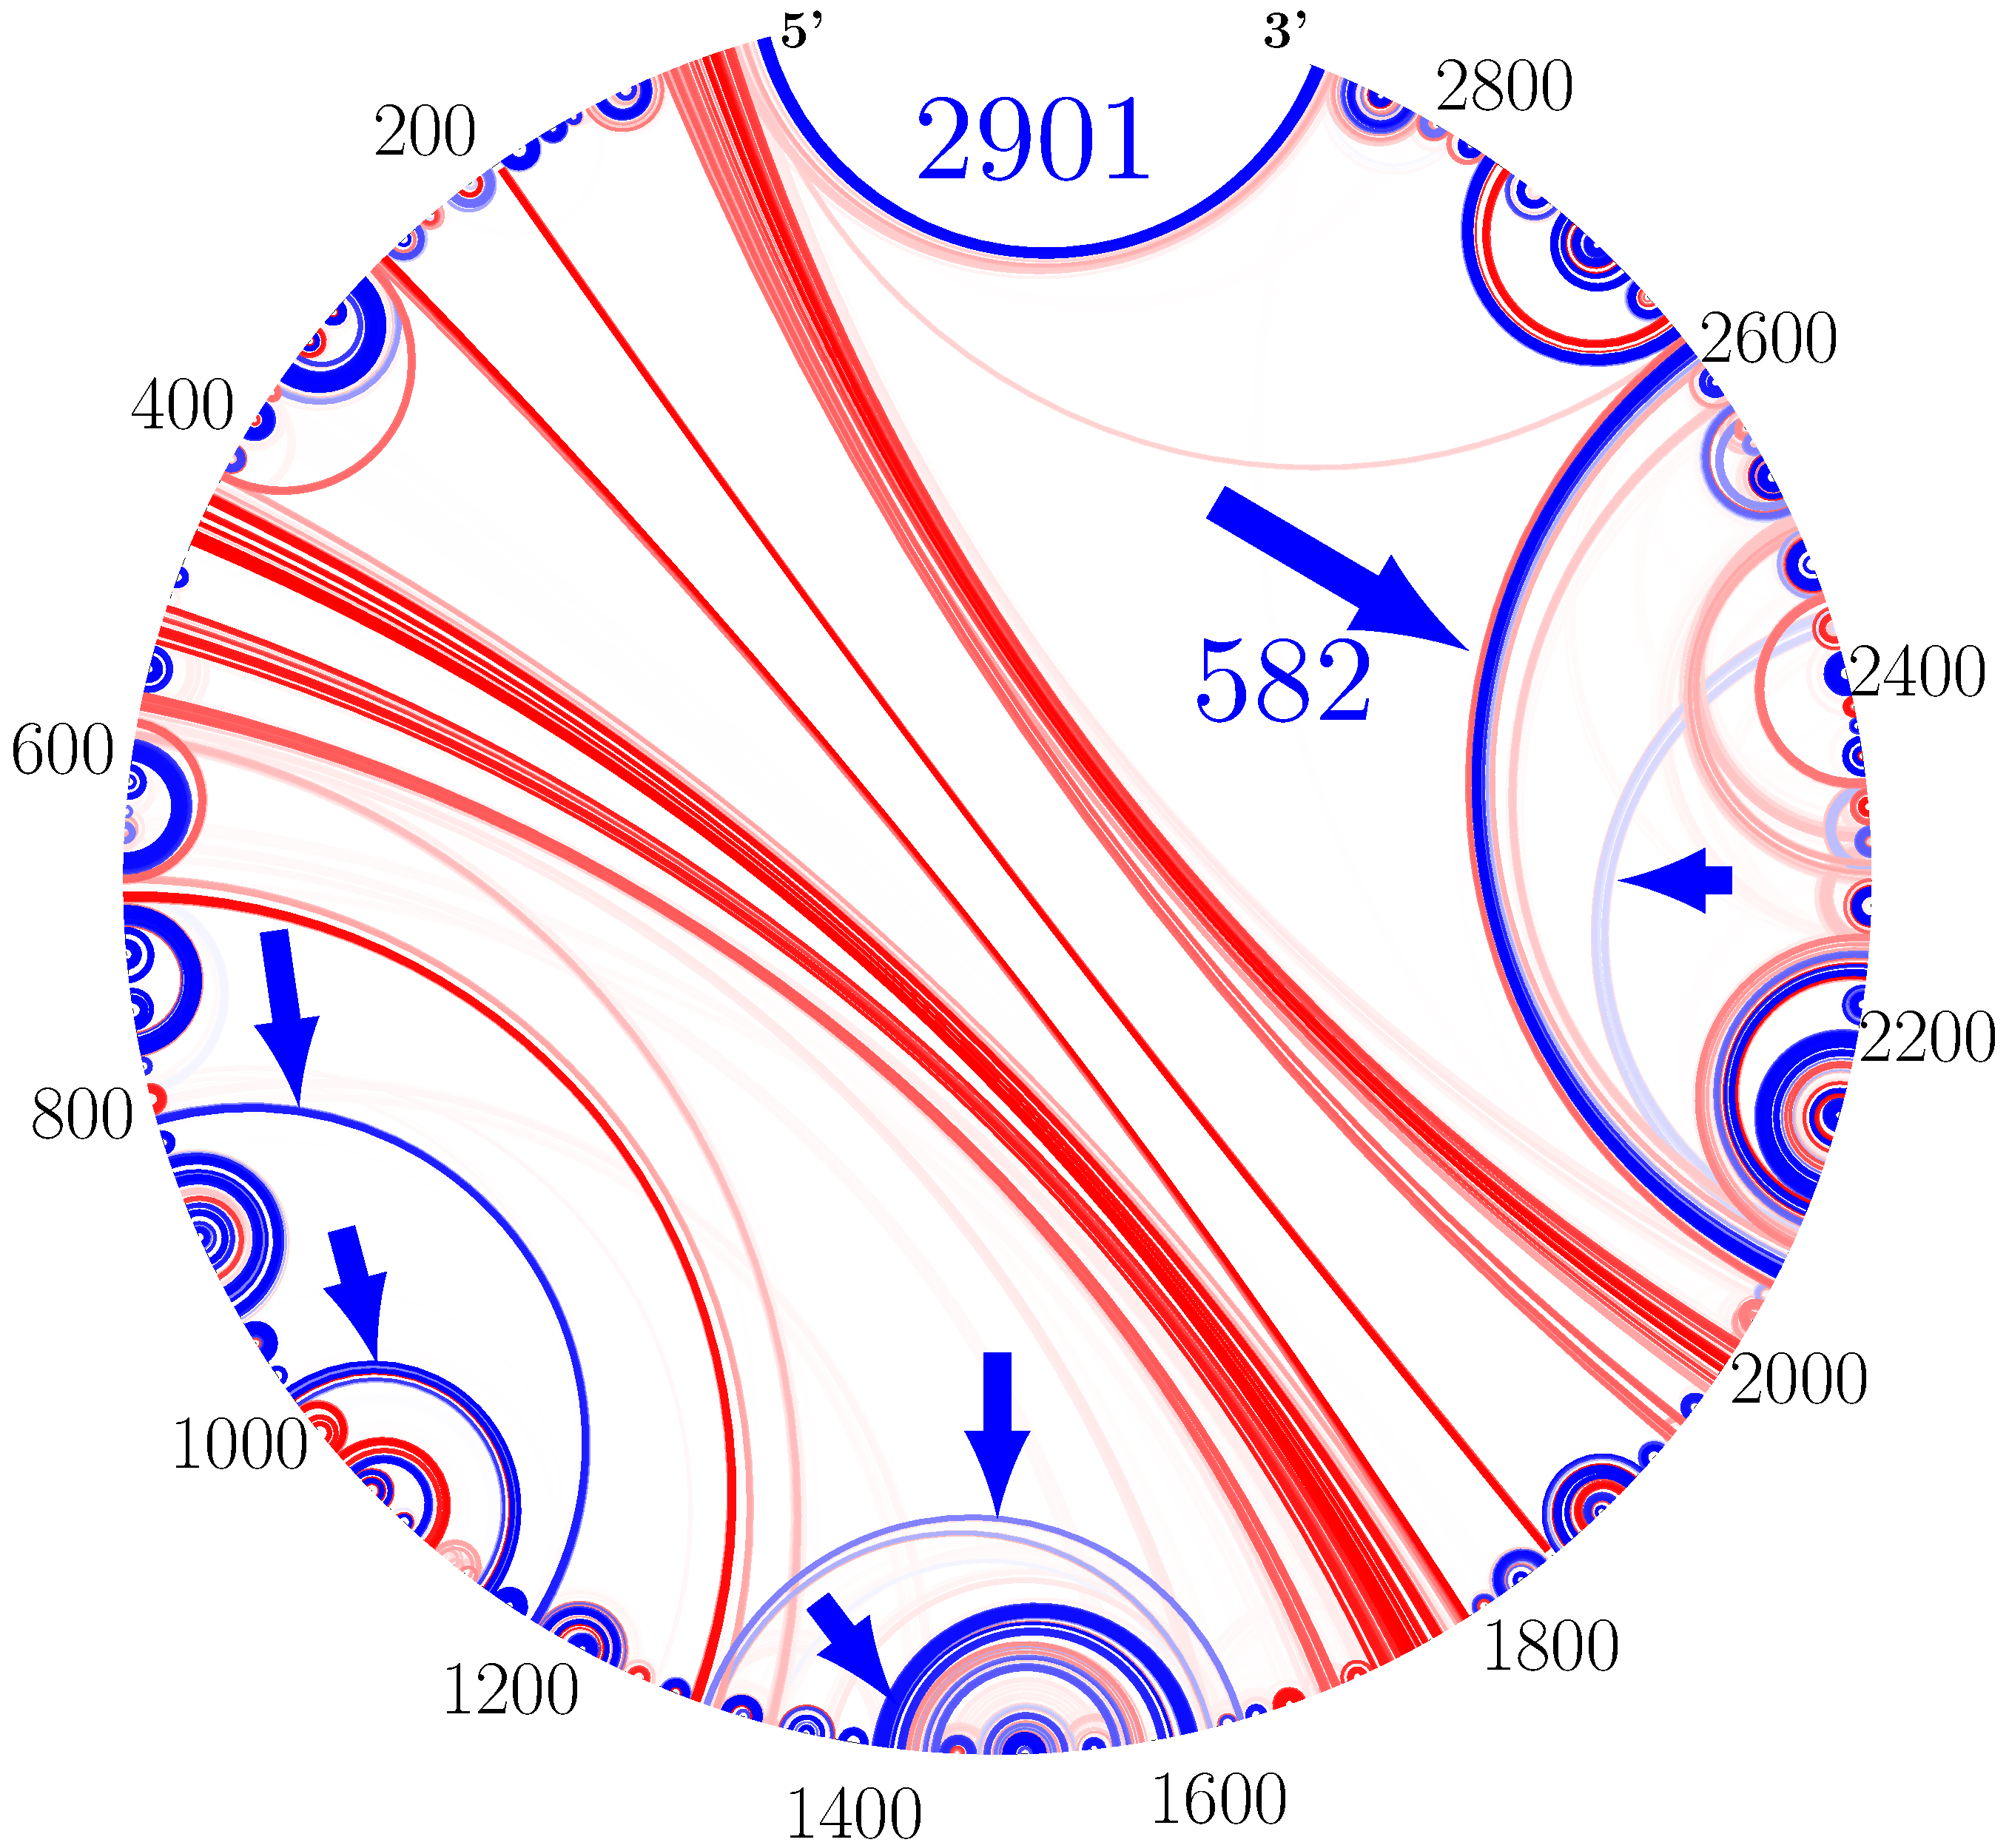
\includegraphics[width=0.25\textwidth]{figs/23s_example.pdf}
% \end{tabular}
\vspace{-2cm}
\caption{
{\bf A--C}: An example of {\it C.~ellipsoidea} Group I Intron. 
{\bf A}: Solid triangles ({\small {\color{blue} $\blacktriangle$} {\color{darkgreen}$\blacktriangle$}  {\color{red}$\blacktriangle$}}) stand for base pairing probabilities and
unfilled circles ({\small {\color{blue} $\circ$} {\color{darkgreen}$\circ$}  {\color{red}$\circ$}})  stand for single-stranded probabilities.
{\color{blue} blue: $p_\linear \!-\! p_\vienna \!>\! 0.2$};
{\color{darkgreen} green: $|p_\linear \!-\! p_\vienna| \!\leq \!0.2$};
{\color{red} red: $p_\linear \!-\! p_\vienna \!<\! -0.2$};
%some high probability pairs and unpaired bases in \linearpartition have low probabilities in \viennarnafold (in blue), and some low probability ones in \linearpartition have high probabilities in \viennarnafold (in red); 
	{\bf B}: Ground truth structure colored with the above scheme; % from \viennarnafold and \linearpartition; 
	%pink binds around position 370 are pseudoknotted pairs.
	{\bf C}: Statistics of this example. 
	"total" columns are the total numbers of triangles and circles with different colors in {\bf A},
	while "correct" columns are the corresponding numbers %of such triangles and circles
        in the ground-truth structure  in {\bf B},
        which is better correlated with \linearpartition's probabilities than \viennarnafold's ({\color{blue} 23 blue pairs} and {\color{red} 0 red pairs}). %ground-truth structure.
	% Note that each triangle represents a pair of nucleotides.
%% {\bf D--G}: An example of \ecoli 23S rRNA. 
%% 	{\bf D}: circular plot of the ground truth.
%% {\bf E--G}: circular plots using the base pair probabilities from \viennarnaplfold (with default window size $70$), \rnafold and \linearpartition, respectively; 
%% base pairs in the ground truth are in blue;
%% the color shade of the lines are propotional to their probabilities.
	\label{fig:example}\\[-.7cm]
}
\end{figure}


\begin{figure*}[hbt!]
\center
\begin{tabular}{@{}c@{}c@{}c@{}c@{}}
\hspace{-4.6cm}\panel{A} & \hspace{-5.2cm}\panel{B} & \hspace{-5.2cm}\panel{C} & \hspace{-2.3cm}\panel{D} 
\\[-0.6cm]
\raisebox{0.35cm}{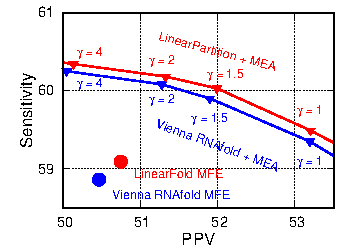
\includegraphics[scale=.8]{figs/LP_MEA_curves}} 
&
%\hspace{-0.5cm}
\hspace{-0.3cm}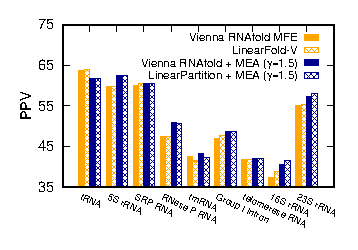
\includegraphics[scale=.93]{figs/MEA_vs_MFE_PPV} 
&
%\hspace{-0.5cm}
\hspace{-0.2cm}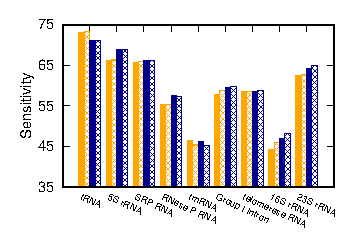
\includegraphics[scale=.93]{figs/MEA_vs_MFE_sens}  
&
\raisebox{.5cm}{\hspace{0.2cm}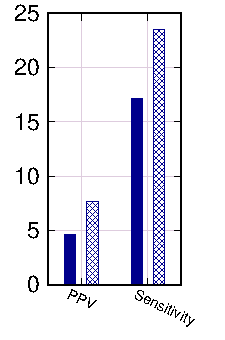
\includegraphics[scale=.56]{figs/bylen_500_mea}}
\\[-0.5cm]
\hspace{-4.6cm}\panel{E} & \hspace{-5.2cm}\panel{F} & \hspace{-5.2cm}\panel{G} & \hspace{-2.3cm}\panel{H} 
\\[-0.5cm]
\raisebox{0.35cm}{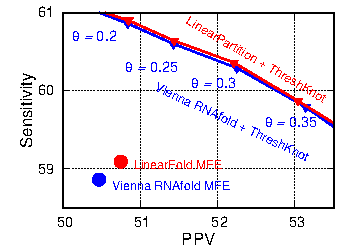
\includegraphics[scale=.8]{figs/LP_ThreshKnot_curves.pdf}}
&
%\hspace{-0.5cm}
       \hspace{-0.3cm}{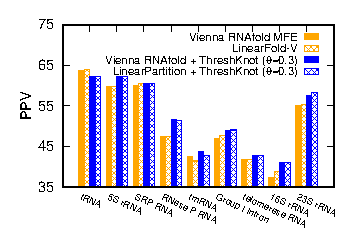
\includegraphics[scale=.93]{figs/new_ThreshKnot_vs_MFE_PPV}}
&
%       \hspace{-0.5cm}
      \hspace{-0.2cm}{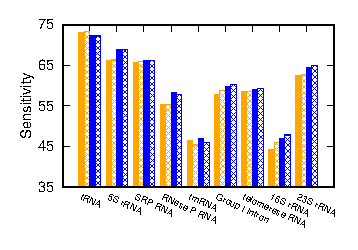
\includegraphics[scale=.93]{figs/new_ThreshKnot_vs_MFE_sens}}
              &
\raisebox{.5cm}{\hspace{0.3cm}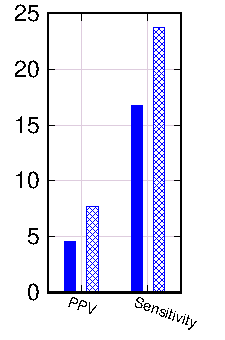
\includegraphics[scale=.56]{figs/bylen_500_threshknot} }
\vspace{-0.6cm}
\end{tabular} % A: specify MFE in label
\caption{Accuracy of downstream  predictions (MEA and \threshknot) using base pairing probabilities from \viennarnafold and \linearpartition
        on the ArchiveII dataset.
	{\bf A}: Overall PPV-Sensitivity tradeoff of MFE (single point) and MEA with varying $\gamma$
	%MFE is a single point, but
        (which can be tuned for higher sensitivity or PPV by adjusting $\gamma$).
	{\bf B} \& {\bf C}: PPV and Sensitivity comparisons of MEA structures for each family.
  {\bf D}: Accuracy comparison of long-distance base pairs (>500 \nts apart) in the MEA structures.
        {\bf E--H}: Same as {\bf A--D}, but using \threshknot predictions instead of MEA.
	%% {\bf D}: Overall PPV-Sensitivity tradeoff of \threshknot with varying threshold $\theta$.
	%% {\bf E} and {\bf F}: PPV and Sensitivity comparisons of ThreshKnot structures for each family.
        %	For easy comparison, {\bf A} and {\bf D} and also {\bf BCEF} are on the same scales.
        We conclude that MEA predictions based on \linearpartitionv are consistently better in both PPV and Sensitivity than
        those based on \viennarnafold for all $\gamma$'s,
        while \threshknot predictions based on those two are almost identical for all $\theta$'s.
        \linearpartitionv is  substantially better on long-distance base pairs in both MEA and \threshknot predictions.
	\label{mea}
        \vspace{-0.6cm}
}
\end{figure*}


Fig.~\ref{fig:ensemble}A--B employs ensemble defect to measure 
the average number %(Fig.~\ref{fig:ensemble_defect}A) 
%and ratio %(Fig.~\ref{fig:ensemble_defect}B) 
of incorrectly predicted nucleotides over the whole ensemble (lower is better).
% ~\cite{Dirks+:2004, Zadeh+:2010}.
\viennarnafold and \linearpartition have similar ensemble defects for short sequences, % are mostly similar between , % are the same or similar,
but \linearpartition has lower ensemble defects for longer sequences, esp.~16S and 23S rRNAs;
in other words, \linearpartition's ensemble has less expected number of incorrectly predicted nucleotides
(or higher number of correctly predicted nucleotides). %, i.e., better correlation with ground-truth structure).
In particular, on 16S and 23S rRNAs, \linearpartition has on average 15.9 and 56.3 more correctly predicted nucleotides than \rnafold,
and on average 8.3 more correctly predicted nucleotides over all families (Fig.~\ref{fig:ensemble}B).
Figs.~\ref{fig:ensemble_defect} show the relative ensemble defects (normalized by sequence lengths),
where the same observations hold, and \linearpartition has on avearge 0.4\% more correctly predicted nucleotides over all families.
In both cases, the differences on tmRNA (worse) and Group I Intron (better) are statistically significant ($p<0.01$).



This finding also implies that  \linearpartition's  base pairing probabilities 
are on average higher than \rnafold's for ground-truth base pairs,
and on average lower for incorrect base pairs.
We use two concrete examples to illustrate this.
First, we plot the ground truth structure of \ecoli 23S rRNA (2,904~\nts) in
Fig.~\ref{fig:ensemble}C,
and then plot the predicted base pairing probabilities
from the local folding tool \viennarnaplfold (with default window size 70), \rnafold, and \linearpartition
in Fig.~\ref{fig:ensemble}D--F, respectively.
We can see that local folding can only produce local pairing probabilities,
while \rnafold misses
most of the long-distance pairs from the ground truth (except the 5'-3' helix),
and includes many incorrect long-distance pairings (shown in red).
By contrast, \linearpartition successfully predicts many
long-distance pairings that \rnafold misses, the longest being 582~\nts apart (shown with arrows).
Indeed, the ensemble defect of this example confirms that \linearpartition's ensemble distribution
has on average 211.4 more correctly predicted nucleotides (over 2,904~\nts, or 7.3\%) than \rnafold's.

As the second example, we use %an RNA sequence,
{\it C.~ellipsoidea} Group I Intron (504~\nts).
First, in Fig.~\ref{fig:ensemble}G--J, we plot the circular plots in the same style as the previous example,
where \linearpartition is substantially better in predicting 4 helices in the ground-truth structure:
[17,24]--[72,79], [30,45]--[66,71], [44,48]--[54,58], and [80,83]--[148,151] (annotated with blue arrows).
%as an example to illustrate this.
% show \linearpartition gives more accurate predicted secondary structure than \viennarnafold.
%compare the base pairing probabilities generated by \viennarnafold and \linearpartition.
Next, in Fig.~\ref{fig:example}A, 
we plot the base pairs (in triangle) and unpaired bases (in circle) 
with \rnafold probability on x-axis and \linearpartition probability on y-axis.
We color the circles and triangles in blue where \linearpartition gives 0.2 higher probability 
than \rnafold %gives low probabilities 
(top left region),
the opposite ones (bottom right region) in red,
and the remainder (diagonal region, with probability changes less than 0.2)
in green.
Then in Fig.~\ref{fig:example}B,
we visualize the ground truth structure~\cite{Cannone+:2002} and color the bases as in Fig.~\ref{fig:example}A.
We observe that the majority of bases are in green, indicating that \rnafold and \linearpartition
agree  with for a majority of the structure features. 
But the blue helices (near 5'-end and [80,83]--[148,151], see also Fig.~\ref{fig:ensemble}J)
indicate that \linearpartition favors these correct substructures by giving them higher probabilities than \rnafold.
We also notice that all red features (where \rnafold does better than \linearpartition) are unpaired bases.
This example shows that although \linearpartition and \rnafold give different probabilities, % compared with \rnafold, 
it is likely that \linearpartition prediction structure is closer to the ground truth structure
(which will be confirmed by downstream structure predictions in Section~\ref{sec:acc}).
The ensemble defect of this example also confirms
that \linearpartition has on average 47.1 more correctly predicted nucleotides (out of 504~\nts, or 9.3\%)
than \rnafold.




Fig.~\ref{fig:example}C gives the statistics of this example.
We can see the green triangles in Fig.~\ref{fig:example}A, 
which denote similar %base pairing
probabilities between \rnafold and \linearpartition, 
are the vast majority. % and the total number is 126,645.
The total number of blue triangles,
for which \linearpartition gives higher base pairing probabilities,
is 55,
and among them 23 %base pairs
(41.8\%) are in the ground truth structure.
On the contrary,
56 triangles are in red,
but none of these \rnafold prefered base pairs are correct. %in the ground truth structure.
% Notice that all the red triangles are on $y=0$ line, 
% for which \linearpartition gives 0 probabilities,
% are in the ground truth structure.
For unpaired bases, 
\linearpartition also gives higher probabilities to more ground truth unpaired bases:
there are 40 blue circles,
among which 37 (92.5\%) are unpaired in the ground truth structure,
while only 19 out of the 44 red circles (43.2\%) are in the ground truth structure.
%% See also Fig.~\ref{fig:ensemble}G--J for another view of this example in the style of Fig.~\ref{fig:ensemble}C--F
%% using circular plots.


\vspace{-0.3cm}
\subsection{Accuracy of Downstream Predictions}%  using Base Pairing Probabilities}
\label{sec:acc}


% \begin{figure}[t!]
% \center
% \begin{tabular}{cc}
% \raisebox{2cm}{\panel{A}} & 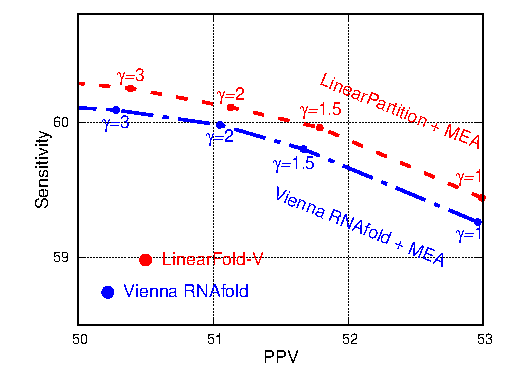
\includegraphics[scale=.7]{figs/new_MEA_diff_gamma_beam_inf_threshold_001} \\[-0.6cm]
% \raisebox{2cm}{\panel{B}} &
% \raisebox{-0.25cm}{\includegraphics[scale=.58]{figs/for_He_Zhang_MEA_gamma_B100}}\\[-0.6cm]
% \raisebox{3cm}{\panel{C}} & \hspace{-0.5cm}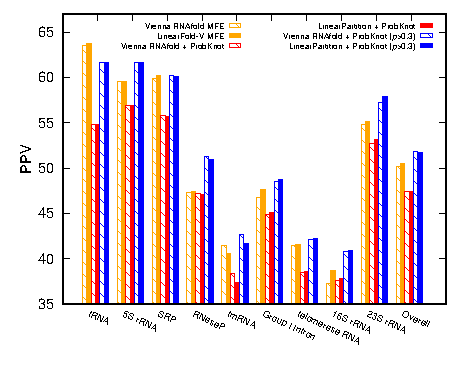
\includegraphics[scale=.78]{figs/ProbKnot_PPV}\\[-0.4cm]
% \raisebox{3cm}{\panel{D}} &\hspace{-0.5cm}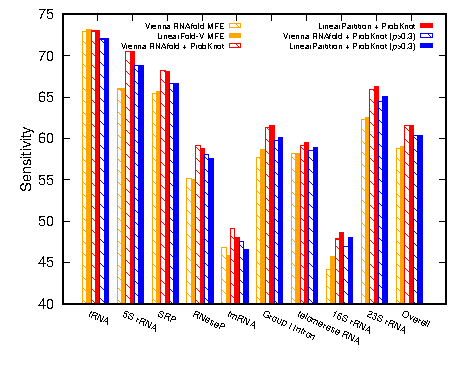
\includegraphics[scale=.78]{figs/ProbKnot_Sens}

% \end{tabular} % A: specify MFE in label
% \caption{Accuracy comparison for two systems.
% 	{\bf A}: Overall MFE and MEA structure PPV-sensitivity tradeoff of two systems with varying $\gamma$. 
% 	{\bf B}: Overall ThreshKnot structure PPV-sensitivity tradeoff of two systems with varying threshold $p$.
% 	{\bf C-D}: PPV and sensitivity comparison for each family.
% 	\label{mea}
% }
% \end{figure}

An important application of the partition function
is to improve structure prediction accuracy (over MFE) using base pairing probabilities.
%These downstream prediction methods include MEA\cite{do+:2006}, \centroidfold~\cite{sato+:2009}, \dotknot~\cite{Sperschneider+Datta:2010}, \probknot~\cite{bellaousov+mathews:2010}, and \ipknot~\cite{sato+:2011},
%have been shown to outperform MFE in accuracy
Here we use two such ``downstream prediction'' methods, MEA\cite{do+:2006} and \threshknot~\cite{Zhang+:2019} which is a thresholded version of \probknot~\cite{bellaousov+mathews:2010},
and compare their results using base pairing probabilities from $O(n^3)$-time baselines and our $O(n)$-time \linearpartition.
%We next consider the accuracy of downstream structure prediction using \linearpartition-produced 
%% First we take base pairing probability matrices from \linearpartition and \viennarnafold (or \contrafold), 
%% feed them to the standard MEA algorithm separately, 
%% and compare the accuracies of prediction structures.
We use Positive Predictive Value (PPV, the fraction of predicted pairs in the known structure, a.k.a.~precision) 
and sensitivity (the fraction of known pairs predicted, a.k.a.~recall) 
as accuracy measurements for each family,
and get overall accuracy be averaging over families. 
% We use slipping method{}
When scoring accuracy, we allow base pairs to differ by one nucleotide in position~\cite{mathews+:1999}.
% ~\cite{sloma+mathews:2016}
We compare \rnafold and \linearpartitionv on the ArchiveII dataset in the main text, and provide the \contrafold vs.~\linearpartitionc comparisons
in the Supporting Information Figs.~\ref{fig:mea_lpc}--\ref{fig:threshknot_lpc}.


% Fig.~\ref{mea} shows that \linearpartition even leads to a small improvement in the downstream MEA predictoin using the probability matrix computed in linear time. 
% Fig.~\ref{mea} gives the accuracy comparison between 
Fig.~\ref{mea}A shows  
MEA predictions (\rnafold + MEA and \linearpartition + MEA) are more accurate than MFE ones (\rnafold MFE and \linearfoldv),
but more importantly,
\linearpartition + MEA  consistently outperforms \rnafold + MEA in both PPV and sensitivity
with the same $\gamma$, a hyperparameter that balances PPV and sensitivity in MEA algorithm.
%\linearpartition + MEA enjoys a small improvement in both PPV and sensitivity.

Figs.~\ref{mea}B--C detail the per-family PPV and sensitivity, respectively,
for MFE and MEA ($\gamma=1.5$) results from Fig.~\ref{mea}A.
% two MFE-based systems and two MEA-based systems for each family
%% for MEA and MFE structures using \rnafold and our \linearfold and \linearpartition.
%% % We can see
%% The MEA
%% % -based systems lead to accuracy improvements over MFE-based systems 
%% structure predictions are more accurate than MFE predictions
%% for most families.
\linearpartition + MEA has similar PPV and sensitivity as \rnafold + MEA on short families (tRNA, 5S rRNA and SRP),
but interestingly, is more accurate on longer families, especially the two longest ones, 16S rRNA (+0.86 on PPV and +1.29 on sensitivity) 
and 23S rRNA (+0.88 on PPV and +0.62 on sensitivity). 
%% We also performed a two-tailed permutation test to test the statistical significance, 
%% and observed that on tmRNA the MEA structures of \linearpartition is significantly worse ($p<0.01$) than \viennarnafold in both PPV and Sensitivity.



% ThreshKnot
%% ProbKnot is another partition function-based structure prediction method that adds a straightforward post-processing step 
%% % after partition function calculation
%% of base pairing probabilities to predict structures
%% and is simpler and faster than MEA~\cite{bellaousov+mathews:2010}.
% Beyond nested structures, ProbKnot can predict pseudoknots. 
\probknot is another downstream prediction method
that is simpler and faster than MEA;
it assembles 
%In ProbKnot, structures are composed of
base pairs with reciprocal highest pairing probabilities. 
Recently, we demonstrated \threshknot~\cite{Zhang+:2019}, 
a simple thresholded version of ProbKnot that only includes pairs that exceed the threshold, 
leads to more accurate %overall 
predictions that outperform MEA by filtering out unlikely pairs, i.e., those whose probabilities fall under a given threshold $\theta$.
%% It has been shown ThreshKnot can achieve better PPV and Sensitivity than the more involved MEA algorithm, 
%% % and can predict pseudoknots which is beyond MEA scope,
%% so we also compare ThreshKnot structure accuracy between \viennarnafold and \linearpartition.


Shown in Fig.~\ref{mea}E, \linearpartition + \threshknot is almost identical in overall accuracy %(slightly better in sensitivity)
to \rnafold + \threshknot at all $\theta$'s,
% in the downstream ThreshKnot prediction using the probability matrix computed in linear time.
%Figs.~\ref{mea}E and F show that \linearpartition + ThreshKnot
and is slightly better than the latter on long families
(+0.24 on PPV and +0.38 on sensitivity for Group I Intron, +0.12 and +0.37 for telomerase RNA, and +0.74 and +0.62 for 23S rRNA)
(Figs.~\ref{mea}F--G).
We also performed a two-tailed permutation test to test the statistical significance, 
and observed that on tmRNA, both MEA and \threshknot structures of \linearpartition are significantly worse ($p\!<\!0.01$) than their \rnafold-based counterparts in both PPV and Sensitivity.
%As was observed for MEA comparison, \linearpartition + ThreshKnot is significantly worse ($p<0.01$) than \viennarnafold on tmRNA.
%in PPV and Sensitivity.


\begin{figure}%[!b]
  \vspace{-.1cm}
\center
%% \iffalse
%% \begin{tabular}{cc}
%% \raisebox{4.6cm}{\panel{A}} & \hspace{-1cm}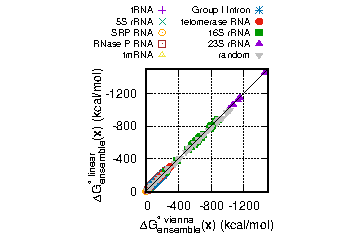
\includegraphics[width=0.3\textwidth]{figs/ensemble_xy} \\
%% % \raisebox{3.6cm}{\panel{B}}
%% \hspace{-1cm}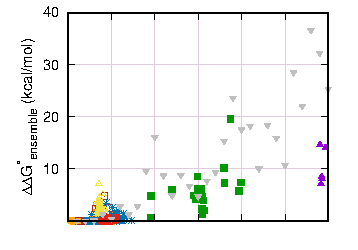
\includegraphics[width=0.2\textwidth]{figs/ensemble_len}
%%  & \hspace{-1cm}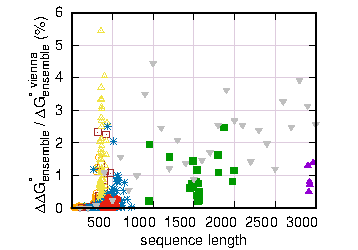
\includegraphics[width=0.2\textwidth]{figs/ensemble_len_norm} \\[-0.3cm]
%% \end{tabular}
%% \fi
%% \iffalse
%% \begin{tabular}{ccc}
%% {\panel{A}} & {\panel{B}} & {\panel{C}} \\
%% \hspace{-1cm}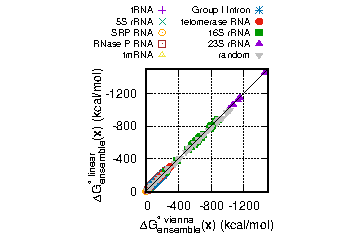
\includegraphics[width=0.3\textwidth]{figs/ensemble_xy} &
%% \hspace{-.8cm}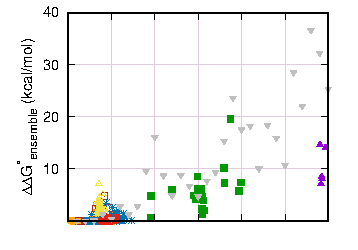
\includegraphics[width=0.3\textwidth]{figs/ensemble_len} &
%% \hspace{-.8cm}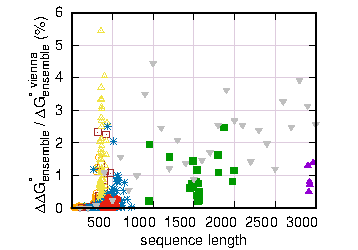
\includegraphics[width=0.3\textwidth]{figs/ensemble_len_norm} \\[-0.3cm]
%% \end{tabular}
%% \fi
\begin{tabular}{cc}
% {\panel{A}} & {\panel{B}}\\
\hspace{-0.2cm}\raisebox{2.9cm}{\panel{A}\hspace{-2.2cm}}\raisebox{2.5cm}{\multirow{2}{*}{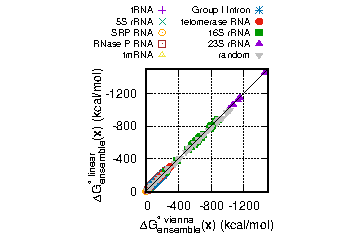
\includegraphics[width=0.47\textwidth]{figs/ensemble_xy}}} & 
\hspace{-2.4cm}\raisebox{2.9cm}{\panel{B}}\hspace{-.35cm}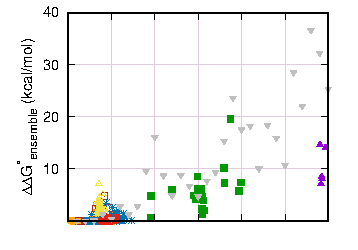
\includegraphics[scale=0.74]{figs/ensemble_len} \\[-.5cm]
% &{\panel{A}}\\
&\hspace{-2.4cm}\raisebox{2.6cm}{\panel{\color{white}C}}\hspace{-.3cm}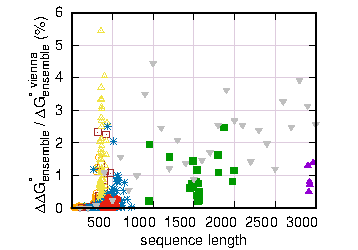
\includegraphics[scale=0.79]{figs/ensemble_len_norm} \\[-0.4cm]
\end{tabular}
\caption{
  Approximation quality of partition function  on ArchiveII dataset and random sequences. %. shorter than 3,000~\nts.
  {\bf A}: The x and y axes are
  ensemble folding free energy changes $\ensenergy(\vecx)$ of \viennarnafold %($-RT\log Q_\vienna(\vecx)$)
  and \linearpartition, % ($-RT\log Q_\linear(\vecx)$),
  respectively.
  {\bf B}: 
  Difference of ensemble folding free energy change (top), ${\ddg(\vecx)}$, between \rnafold and \linearpartition.
  and the relative differences (bottom),  ${\ddg(\vecx)}/{\ensenergyvienna(\vecx)}$, in percentages.
  %% of 
  %% ensemble folding free energy changes,
%  $\frac{ \ensenergyvienna(\vecx) - \ensenergylinear(\vecx)}{\ensenergylinear(\vecx)}$.
  \label{fig:partition}
  \vspace{-0.2cm}
}
\end{figure}


Fig.~\ref{mea}D \& H show that \linearpartition-based predictions are subtantially better than \rnafold's (in both PPV and sensitivity) for long-distance base pairs (those with 500+ \nts apart),
which are well known to be challenging for the current models.
Fig.~\ref{fig:distance} details the accuracies on base pairs with different distance groups.


Figs.~\ref{fig:mea_lpc}--\ref{fig:threshknot_lpc} show similar comparisons between 
\contrafold and \linearpartitionc using MEA and ThreshKnot prediction, %, separately. 
% Fig.~\ref{fig:mea_lpc} compares MEA structures ($\gamma>1.5$) accuracy based on these two systems and Fig.~\ref{fig:threshknot_lpc} compares ThreshKnot structures ($p>0.2$). 
with similar results to Fig.~\ref{mea}, i.e., downstream structure prediction using \linearpartitionc is as accurate as using \contrafold, and  (sometimes significantly) more accurate on longer families.


\iftrue
%<<<<<<< HEAD
\begin{figure*}[!h]
%\vspace{-0.2cm}
%% =======
%% \begin{figure*}[!ht]
%% \vspace{-0.5cm}
%% >>>>>>> e07b35b96f33f564a07e21f062362ad3acd7bbad
\center
\begin{tabular}{cc|c}
\hspace{-5.5cm}\panel{A} & \hspace{-6.cm}\panel{B} & \hspace{-5.2cm}\panel{E} \\[-0.5cm]
\hspace{-0.5cm}\includegraphics[width=0.33\textwidth]{figs/tRNA_identical_heatmap}
&
% \hspace{-0.8cm}{\includegraphics[width=0.33\textwidth]{figs/rmsd_family_plus_random_b2}}
\hspace{-1.1cm}{\includegraphics[width=0.33\textwidth]{figs/rmsd_archiveII_rnacentral_lpv_float_plus_long_random}}
% \\[-0.2cm]
&
% \panel{C} & \panel{D}\\[-0.5cm]
\hspace{0.2cm}\includegraphics[width=0.33\textwidth]{figs/overall_average_change_prob} \\[-0.1cm]

\hspace{-5.5cm}\panel{C} & \hspace{-6.cm}\panel{D} & \hspace{-5.2cm}\panel{F} \\[-0.5cm]
\hspace{-.8cm}\raisebox{-0.2cm}{\includegraphics[width=0.35\textwidth]{figs/structure_entropy_xy_plus_random_rnacentral}}
&
\hspace{-0.7cm}\includegraphics[width=0.33\textwidth]{figs/sorted_prob_23s} 
&
\hspace{-0.0cm}\includegraphics[width=0.34\textwidth]{figs/overall_vienna_prob_bin_count}  \\[-0.2cm]
\end{tabular}
\caption{
Comparison of base pairing probabilities from \viennarnafold and \linearpartition.
	{\bf A}: \linearpartition (upper triangle) and Vienna RNAfold (lower triangle) result in identical base pairing probability matrix for \ecoli tRNA$^\textit{Gly}$.
	{\bf B}: The root-mean-square deviation, $\RMSD(p_\vienna, p_\linear)$, is relatively small between \linearpartition and Vienna RNAfold; all tRNA and 5S rRNA sequences \RMSD is close to 0 (e.g., RMSD$<10^{-5}$).
	{\bf C}: Average positional structural entropy $H(p)$ comparison; \linearpartition has noticeably lower entropy.
	{\bf D}: \linearpartition starts higher and finishes lower than \viennarnafold in a sorted probability curve for \ecoli 23S rRNA,
        suggesting lower entropy.
	{\bf E}: Mean absolute value of change in base pairing probabilities between \viennarnafold and \linearpartition; these changes are averaged within every probability bin.
	{\bf F}: Pair probability distribution of \viennarnafold. 
	Note that the y-axis is limited to 50,000 counts, and the counts of first three bins (with probability smaller than 3\%) are far beyond 50,000.
	\label{fig:rmsd}
}
\vspace{-0.3cm}
\end{figure*}
\fi



\vspace{-0.2cm}
\subsection{Approximation Quality (Default Beam Size)}

\linearpartition uses beam pruning to ensure $O(n)$ runtime, % and linear space, % linearity, 
thus is approximate compared with standard $O(n^3)$-time algorithms.
% Fig. 4A–B show that our \linearpartition algorithm can indeed approximate the partition function reasonably well.
We now investigate its approximation quality at the default beam size~100.

First, in Fig.~\ref{fig:partition}, we measure the approximation quality of the partition function calculation,
%and specifically,
in particular,  the ensemble folding free energy change (also known as ``free energy of the ensemble'')
which reflects the size of the partition function, 
\[
\ensenergy (\vecx) = -RT \log Q(\vecx).
\]
Fig.~\ref{fig:partition}A shows that the \linearpartition 
% free energy of ensemble 
estimate for the ensemble folding free energy change
is close to the \rnafold estimate 
on the ArchiveII dataset and randomly generated RNA sequences.
The similarity shows that little magnitude of the partition function is lost by the beam pruning. 
For short families, free energy of ensembles between \linearpartition and \rnafold are almost the same.
For 16S and 23S rRNA sequences and long random sequences (longer than 900 nucleotides), 
\linearpartition gives a lower magnitude ensemble free energy change, 
but the difference,
\[
\ddg(\vecx) = \ensenergyvienna(\vecx) - \ensenergylinear(\vecx) \, \geq 0
\]
is smaller than 20 kcal/mol for 16S rRNA, 
15 kcal/mol for 23S rRNA,
and 37 kcal/mol for random sequences (Fig.~\ref{fig:partition}B). 
The maximum difference for random sequence is larger than natural sequences (by 17.2 kcal/mol).
This likely reflects the fact that random sequences tend to fold less selectively to probable structures~\cite{Fu+:2015},
and the beam is therefore pruning structures in random that would contribute to the overall folding stability.
% Fig.~\ref{ensemble} confirms \linearpartition approximation quality of partition function is good.
Fig~\ref{fig:partition}C shows the ``relative'' differences in ensemble free energy changes,
 ${\ddg(\vecx)}/{\ensenergyvienna(\vecx)}$,
are also very small: only up to 2.5\% and 1.5\% for 16S and 23S rRNAs, and up to 4.5\% for random sequences.



Next, in Fig.~\ref{fig:rmsd}, we measure the approximation quality of base pairing probabilities using root-mean-square deviation (\RMSD)
between two probability matrices $p$ %(from cubic algorithms, for example, \viennarnafold) 
and $p'$ %(from our algorithm, for example, \linearpartition)
%(i.e., $p_\vienna$ and $p_\linear$)
over the set of all possible Watson-Crick and wobble pairs on a sequence $\vecx$.
We  define
\begin{equation}
  \vspace{-0.4cm}
\begin{split}
  {\pairings}(\vecx) \!=\!\{  &1\leq i <j\leq |\vecx| \bigm\vert j-i>3 \\[-0.1cm]
    &  \vecx_i\vecx_j \in \{\text{\small CG, GC, AU, UA, GU, UG}\}\!\} \notag
\end{split}
\end{equation}
\vspace{-0.2cm}
and:\vspace{-0.05cm} 
\begin{equation}
\RMSD(p,p')\!=\!\!\!\sqrt{\frac{1}{|{\pairings}(\vecx)|} \sum_{(i,j) \in {{\pairings}(\vecx)}}{\!\!\!\!\!(p_{i,j}\!-\!p'_{i,j})}^2}\notag
\end{equation}

\begin{figure*}[!h]
  \vspace{-0.7cm}
\center
\begin{tabular}{cccc}
% \hspace{-5.cm} \panel{A} & \hspace{-5.2cm}\panel{B}  \\[-0.2cm]
\raisebox{3.7cm}{\panel{A}} & 
\hspace{-0.5cm}\includegraphics[width=0.4\textwidth]{figs/ensemble_beamsize_overall} &
\raisebox{3.7cm}{\panel{B}} &
\hspace{-0.5cm}{\includegraphics[width=0.4\textwidth]{figs/RMSD_beamsize_overall}}
\end{tabular}
\\[-1.2cm]
\begin{tabular}{c@{}c@{}c@{}c@{}c@{}c}
% \hspace{-5.cm}\panel{C} & \hspace{-5.2cm}\panel{D} & \hspace{-5.8cm}\panel{E} \\[-0.2cm]
\hspace{0.6cm}\raisebox{3.8cm}{\panel{C}} & 
\hspace{-1cm}\includegraphics[width=.35\textwidth]{figs/precision-recall-overall-lpv} 
&
\hspace{-.5cm}\raisebox{3.8cm}{\panel{D}} & 
\hspace{-1.2cm}\includegraphics[width=0.35\textwidth]{figs/precision-recall-tmRNA-lpv-hzhang}
&
\hspace{-0cm}\raisebox{3.8cm}{\panel{E}} & 
\hspace{-1.5cm}\includegraphics[width=0.35\textwidth]{figs/precision-recall-16s-lpv-hzhang}
\vspace{-0.4cm}
\end{tabular}
\caption{
Impact of beam size. 
{\bf A}: Relative difference of 
  ensemble folding free energy change, $\ddg/\Delta G^\circ_\text{ensemble}$, against  beam size. %, averaged over all families.
{\bf B}: RMSD against beam size. %, averaged over all families.
{\bf C}: Overall PPV and Sensitivity with beam size.
{\bf D--E}: tmRNA and 16S rRNA PPV and Sensitivity against beam size, respectively. 
%{\bf E}: 16S rRNA PPV and Sensitivity change with beam size. 
Note that the  results of \threshknot using \rnafold (yellow triangles in {\bf C--E}) are identical to \threshknot using
the {\em exact} version of \linearpartition ($b\!=\!\infty$).
%since \linearpartition with infinite beam size (i.e., no beam pruning) does $O(n^3)$ exact partition function calculation as \viennarnafold.
\label{fig:beamsize}
\vspace{-0.7cm}
}
\end{figure*}


Figs.~\ref{fig:rmsd}A and B confirm that our \linearpartition algorithm (with default beam size 100) can indeed approximate the base pairing probability matrix reasonably well. 
Fig.~\ref{fig:rmsd}A shows the heatmap of probability matrices for {\it E.~coli} tRNA$^\textit{Gly}$. 
\rnafold (lower triangle) and \linearpartition (upper triangle)
yield identical matrices (i.e., $\RMSD=0$). % (i.e., RMSD$\approx$0). 
Fig.~\ref{fig:rmsd}B shows that the \RMSD of each sequence in ArchiveII and RNAcentral datasets, 
and randomly generated artificial RNA sequences, %with length 100–16,000~\nts.
is relatively small. % across all sequences. 
% To verify approximation quality of 
The highest deviation is 0.065 for {\it A.~truei} RNase P RNA, 
which means on average 
each base pair's probability deviation in that worst-case sequence is about 0.065 between the cubic algorithm (\rnafold) and our linear-time one (\linearpartition). 
On the longest 23S rRNA family, the \RMSD is about 0.015. 
We notice that tmRNA is the family with biggest average \RMSD. %, and its accuracy is also the worst.
The random RNA sequences behave similarly to natural sequences in terms of \RMSD, 
i.e., \RMSD is  close to 0 ($\!<\!10^{-5}$) for short ones, then becomes bigger around length 500 and decreases after that, 
but for most cases their \RMSD's are slightly larger than  
the natural sequences. %in similar length range.
This indicates that the approximation quality is relatively better for natural sequences.
For RNAcentral-sampled sequences, \RMSD's are all small and around 0.01.

% With sequence length increasing, RMSD gradually decreases, 
% since the number of possible pairs grows in $O(n^2)$ but the number of highly probable pairs grows in $O(n)$. 
% To avoid RMSD is dominented by most base pairs with small probabilities,
% we consider a more strict circumstance. 
% Instead of divided by the number of all possible base pairs,
% We only consider the ones which have probability $p>0.01$.
% The RMSD resutls with such constrain are presented in Fig.~\ref{fig:rmsd_threshold}.
% It shows that for sequence shorter than 300$nt$, RMSD($p>0.01$) is still 0. 
% This also confirms that our \linearpartition gives exactly the same probability matrix as cubic algorithm.
% RMSD($p>0.01$) fluctuates from 0 to about 0.43 for sequences whose lengthes are in the range [300,1000]. Beyond 1,000$nt$, RMSD($p>0.01$) becomes stable between 0.2 and 0.4.



% Fig.~\ref{fig:rmsd}C and D show
We hypothesize that \linearpartition reduces the uncertainty of the output  distributions %(both base pairing probabilities distribution
%is shifted to higher probability 
because it filters out states with lower partition function.
We measure this using average positional structural entropy $H(p)$, %$~\cite{Garcia-Martin+Clote:2015}, 
% which is defined as:
which is the average of positional structural entropy $H_2(i)$ for each nucleotide $i$~\cite{Huynen+:1997,Garcia-Martin+Clote:2015}:
\vspace{-0.2cm}
\begin{equation}
  \vspace{-0.3cm}
\begin{split}
H(p) &= \frac{1}{n}\sum_{i=1}^{n}{H_2(i)} =\frac{1}{n}\sum_{i=1}^{n}({-\sum_{j=0}^{n}p_{i,j}\mathrm{log}_{2}p_{i,j}}) \\
		&=-\frac{1}{n}\sum_{i=1}^{n}{\sum_{j=0}^{n}p_{i,j}\mathrm{log}_{2}p_{i,j}} \notag
\end{split}
\end{equation}
where $p$ is the base pairing probability matrix,
% in which 
%$p_{i,j}$ is the probability of nucleotide $i$ paired with $j$ when $j\neq 0$, 
and $p_{i,0}$ is the probability of nucleotide $i$ being unpaired ($q_i$ in Eq.~\ref{eq:phi}).
%$n$ is the sequence length.
The lower entropy indicates that the distribution is dominated by fewer base pairing probabilities.
Fig.~\ref{fig:rmsd}C confirms \linearpartition distribution shifted to higher probabilities (lower average entropy) than \rnafold for most sequences.

Fig.~\ref{fig:rmsd}D uses \ecoli 23S rRNA to exemplify the difference in base pairing probabilities.
We sort all these probabilities from high to low and take the top 3,000.
The \linearpartition curve starts higher and finishes lower, confirming a lower entropy. %the distribution shifts to higher probabilities. % (rich get richer).



% E F
Figs.~\ref{fig:rmsd}E and F follow a previous analysis method~\cite{Zuber+:2017} to estimate the approximation quality with a different perspective. 
We divide the base pairing probabilities range [0,1] into 100 bins, i.e., the first bin is for base pairing probabilities [0,0.01), and the second is for [0.01, 0.02), so on so forth. 
In Fig.~\ref{fig:rmsd}E we visualize the averaged change of base pairing probabilities between \rnafold and \linearpartition for each bin.
We can see that larger probability changes are in the middle (bins with probability around 0.5),
and smaller changes on the two sides (with probability close to either 0 or 1).
%while both on the left (bins with probability near 0) and on the right (bins with probability near 1) the changes are smaller.
In Fig.~\ref{fig:rmsd}F we illustrate the counts in each bin based on \rnafold base pairing probabilities.
We can see that most base pairs have low probabilities (near 0) or very high probabilities (near 1).
Combine Figs.~\ref{fig:rmsd}E and F together, we can see that probabilities of most base pairs are near 0 or 1, where the differences between \rnafold and \linearpartition are relatively small. 
Fig.~\ref{fig:bin_counts} provides the comparison of counts in each bin between \rnafold and \linearpartitionv. The count of \linearpartitionv in bin [99,100) is slightly higher than \rnafold, 
while the counts in bins near 0 (being capped at 50,000) are much less than \rnafold.
This  also confirms that \linearpartition prunes base pairs with tiny probabilities.



\vspace{-0.4cm}
\subsection{Adjustable Beam Size}

Beam size in \linearpartition is a user-adjustable hyperparameter controlling beam prune, 
and it balances the approximation quality and runtime.
A smaller beam size shortens runtime, but sacrifices approximation quality.
With increasing beam size, \linearpartition gradually approaches the classical $O(n^3)$-time algorithm and 
the output is finally identical to the latter when the beam size is $\infty$ (no pruning).
Fig.~\ref{fig:beamsize}A shows the changes in approximation quality of the ensemble free energy change,
$\Delta G^\circ_\text{ensemble}(\vecx)$, with $b=20\rightarrow 800$.
Even with a small beam size ($b=20$) the difference is only about 5\%, which quickly shrinks to 0 as $b$ increases.
Fig.~\ref{fig:beamsize}B shows the changes in \RMSD with changing $b$. %=20\rightarrow 800$.
% We use averaged length and averaged RMSD for each family with a certain beam size.
%We observe that \RMSD decreases when beam size increases. 
With a small beam size $b=20$ the average \RMSD is lower than 0.035
over all ArchiveII sequences,
which shrinks to less than 0.005 at the default beam size ($b=100$),
and almost 0 with $b=500$.% the average \RMSD is
% and tmRNA remains relatively high averaged RMSD compared with other short families.
% This is consistant with Fig.~\ref{fig:rmsd}B.
%% With a larger beam size, $b=500$, 
%% % which means no beam prune for partition function calculation, 
%% the average \RMSD decreases to almost 0.
% It is also clear that shorter families' averaged RMSD decreases faster. 


Beam size also has impact on PPV and Sensitivity.
Fig.~\ref{fig:beamsize}C gives the overall PPV and Sensitivity changes with beam size.
We can see both PPV and Sensitivity improve from $b=50$ to $b=100$,
and then become stable beyond that.
%Therefore, we choose beam size 100 as the default beam size.
Figs.~\ref{fig:beamsize}D and E present this impact for two selected families.
% tmRNA is the worst family in the sense of accuracy for \linearpartition.
Fig.~\ref{fig:beamsize}D shows tmRNA's PPV and Sensitivity both increase when enlarging beam size.
Using beam size 200, \linearpartition achieves similar PPV and Sensitivity as \rnafold.
% This indicates that it is better to use a larger beam size, for example, $b=200$ when running 
% \linearpartition on tmRNA sequence.
However, increasing beam size is not benefical for all families.
% especially for long families.
Fig.~\ref{fig:beamsize}E gives the counterexample of 16S rRNA. 
We can see both PPV and Sensitivity decrease with $b$ from 50 to 100.
After that, Sensitivity drops with no PPV improvement.
% PPV increases while Sensitivity decreases when changing beam size from 100 to 120. 
% Continue increasing beam size, Sensitivity drops with no PPV improvement.

\smallskip
% discussion about k-best parsing
\linearfold uses $k$-best parsing~\cite{huang+:2005} to reduce runtime from $O(nb^2)$ to $O(nb{\mathrm {log}}b)$ without losing accuracy.
% Basically, $k$-best parsing is to find the top-$k$ states 
% The reason of the difference is that 
Basically, 
$k$-best parsing is to find the exact top-$k$ (here $k\!=\!b$) states out of $b^2$ candidates
% with no need of approximation
in $O(b{\mathrm {log}}b)$ runtime.
%by using a heap.
% instead of .
% while the naive algorithm needs to 
If we applied $k$-best parsing here,
\linearpartition would sum the partition function of only these top-$b$ states
instead of the partition function of $b^2$ states.
This change would introduce a larger approximation error,
especially when the differences of partition function between the top-$b$ states 
and the following states near the pruning boundary are small.
Therefore, in \linearpartition we do not use $k$-best parsing as in \linearfold,
and the runtime is $O(nb^2)$ instead of $O(n b\log b)$.
% For \linearfold, since it only needs to predict one MFE structure,
% the rest candidates are much less promising to be part of the MFE structure.
% However, \linearpartition needs to consider the ensumble at equilibrium, 
% so the partition function of the candidate states may also make unneglactable contributions to total partition function.

% \begin{figure}[b]
% \center
% \includegraphics[width=0.48\textwidth]{figs/RMSD_beamsize}
% \caption{
% Impact of beam size. Add beamsize-accuracy figures???
% 	\label{fig:beamsize}.
% }
% \end{figure}



%\subsection{Example}


Finally, we note that the default beam size $b\!=\!100$ follows \linearfold and %is a simple round number;
we do not tune it.
